\documentclass{article}

% \usepackage[margin=1in,includefoot]{geometry}
\usepackage{graphicx}
\usepackage{titlesec}
\usepackage[table]{xcolor}
\usepackage{color, colortbl}
\usepackage{stackengine}
\usepackage{fancyhdr}
\usepackage{longtable}
\usepackage{changepage}
\usepackage{tikz, graphicx}

\newcommand\xrowht[2][0]
{\addstackgap[.5\dimexpr#2\relax]{\vphantom{#1}}}
% \newcolumntype{C}{>{\centering\arraybackslash}p{0.6cm}}
% \newcolumntype{D}{>{\centering\arraybackslash}p{10cm}}
% \setlength{\parskip}{1em}

\setlength{\arrayrulewidth}{0.4mm}
\setlength{\tabcolsep}{20pt}
\renewcommand{\arraystretch}{1.6}
\setcounter{tocdepth}{4}
\setcounter{secnumdepth}{4}

\pagestyle{fancy}
\renewcommand{\headrulewidth}{2pt}
\renewcommand{\footrulewidth}{1pt}

\begin{document}
\begin{titlepage}
	\begin{center}
		\begin{figure}
			\centering
			
\includegraphics[scale=0.3]{LogoPolimi.PNG} \\
			[0.3cm]
		\end{figure}
		\Huge{\bfseries - RASD -} \\
		[0.5cm]
		\huge{Requirements Analysis and
			
			Specification Document} \\
		[1mm]
		\rule{300pt}{3pt} \\
		[1.0cm]
		\textsc{\Large Computer Science and Engineering} \\ 
		\textsc{\Huge Software Engineering II} \\
		\textsc{\Large A.A. 2020/2021} \\
		[1cm]
		\textsc{\LARGE Daniele Mammone - 10625264} \\
		\textsc{\LARGE Gianmarco Naro - 10610374} \\
		\textsc{\LARGE Massimo Parisi - 10583470} \\
	\end{center}
\end{titlepage}

\newpage
	
	\renewcommand\contentsname{Contents}
	\tableofcontents
	
\newpage

\section{Introduction}

	\subsection{Purpose}
	
	The main target of this document is to describe the software through functional and non-functional requirement and is used as contractual basis between the customer and the developer. The structure of the document follows the one studied during lectures and aim to describe faithfully the software behaviour in all of its aspects.
	
	The software in question is \emph{CLup}, a mobile service usable through app, made both for store managers and customers. It facilitates customers to book a visit to a store and, on the other hand, to help store managers to observe the new strict rules due to \emph{Covid-19}.
	
	\subsection{Scope}
	
	The main purpose of \emph{CLup} is to facilitate customers to access at a store in {\bfseries security}, both allowing them to reserve a spot on the queue for entering the store through the app and to book a visit at the store in a determined time window, selected by the user. Thanks to this, store managers can manage the {\bfseries affluency} in their store more easilier, and moreover can reduce the crowd in front of the store, that is the main purpose of the application. The main idea is that when a person's number is called, he can enter the supermarket. Moreover, the app should generate a \emph{QR Code} that the customer will scan at the entry and at the exit of the store, so that the system knows in real time how many people there are in the store. \emph{CLup} should also estimates the \emph{ETA} from the turn of a person. Moreover, it is able to suggest people other store options when there is a high waiting time to enter to the store requested by the user. The app also allows people to reserve their spot at the supermarket and, in order to optimize the waiting time, people can select specifics departments where they want to go in the store.
	
	Summing up, \emph{CLup} has this main functionalities:
	
	\smallskip
	
	\begin{itemize}
		
		\item {\bfseries Manage of lining up of the store}: the app will manage the accesses to the store, based on numbered tickets released to people. When it's the turn of a person, it will be authorized to enter the shop. Futhermore, the store manager is able to manage the access and the affluency to the store.
		
		\item {\bfseries Booking visit}: users can book a visit at the store, in a certain time frame decided in the booking process. For them, there is no requirement of ticket, since are able to access the store only scanning the \emph{QR Code} at the store entrance. The system will grant access if the time of entering is correct.
		
		\item {\bfseries Alternatives}: the app is able to suggest other stores options and time if some store is full, or comfortable times aren't available at the moment of the booking.
	
	\end{itemize}

	%Following this brief introduction of the application scope, there are %the Phenomenon involved in the system.
		
		\subsubsection{World Phenomena}
		
		\bigskip
		
		\begin{center}
			
			\rowcolors{2}{}{gray!20}
			\rowcolors{1}{gray!20}{white}
			\renewcommand{\arraystretch}{2.5}
		
			\begin{adjustwidth}{-1.5cm}{}
			\begin{tabular}[h!]{|m{2.5em}|m{32.5em}|}
				
				\hline
				\xrowht{5pt}
				WP1 & A user enters a supermarket \\
				\xrowht{5pt}
				WP2 & A user waits in a lineup \\
				\xrowht{5pt}
				WP3 & A user exits the supermarket \\
				\xrowht{5pt}
				WP4 & A certain number of people is inside the supermarket \\
				\xrowht{5pt}
				WP5 & A certain number of people is at a specific department of the supermarket \\
				\hline
			\end{tabular}
			\end{adjustwidth}
		
		\end{center}
	
		\smallskip
		
		\subsubsection{Shared Phenomena}
		
		\bigskip
		
		\begin{center}
			
			\rowcolors{2}{}{gray!20}
			\rowcolors{1}{gray!20}{white}
			\renewcommand{\arraystretch}{2.5}
			
			\begin{adjustwidth}{-1.5cm}{}
			\begin{tabular}[h!]{|m{2.5em}|m{27.5em}|m{1em}|}
				
				\hline
				\xrowht{5pt}
				SP1 & The user gets a ticket/QR & M\\
				\xrowht{5pt}
				SP2 & The user books a visit to the store & M\\
				\xrowht{5pt}
				SP3 & The store generates in presence a ticket & M\\
				\xrowht{5pt}
				SP4 & The user comes to knows how much time they have to wait before entering & U\\
				\xrowht{5pt}
				SP5 & The users know how many people there are in a store at a certain moment & U\\
				\xrowht{5pt}
				SP6 & The user scan the QR code and enters in the supermarket & U\\
				\xrowht{5pt}
				SP7 & The user scan the QR code and exits from the supermarket & U\\
				\xrowht{5pt}
				SP8 & The user can indicate the categories of items that he intend to buy & U\\
				\hline
				
			\end{tabular}
			\end{adjustwidth}
		
		\end{center}
		
		\subsubsection{Goals}
		
		\bigskip
		
		\begin{center}
			
			\rowcolors{2}{}{gray!20}
			\rowcolors{1}{gray!20}{white}
			\renewcommand{\arraystretch}{2.5}
			
			\begin{adjustwidth}{-1.5cm}{}
			\begin{tabular}[h!]{|m{2.5em}|m{32.5em}|}
				
				\hline
				\xrowht{5pt}
				G1 & Allow customers to select a store and book a spot on the queue from \emph{CLup} app \\
				\xrowht{5pt}
				G2 & Allow customers to select a store and take a spot on the queue to enter as soon as possible the store from \emph{CLup} app \\
				\xrowht{5pt}
				G3 & Allow customers to book a spot on the queue from a physical ticket dispenser \\
				\xrowht{5pt}
				G4 & Allow customers to select a better store option to avoid waisting a lot of time waiting to entry at a specific store \\
				\xrowht{5pt}
				G5 & Allow customers to decrease waiting times specifing departments they want to visit \\
				\xrowht{5pt}
				G6 & Allow customers users to manage their spots on the queue and their reservation \\
				\xrowht{5pt}
				G7 & Allow customers to depart from their location in time to avoid waiting too much, and to avoid losing their turn in lineup \\
				\xrowht{5pt}
				G8 & Allow store managers to decide how many people, and how many booked clients to have in the store and in which department \\
				\xrowht{5pt}
				G9 & Allow the store manager to know the real situation of people that are inside the building and in which department of his store \\
				\xrowht{5pt}
				G10 & Allow to grant a fair managment of users that can access the building \\
				\xrowht{5pt}
				G11 & Allow to manage optimally the influx in the building and avoid gathering inside it \\
				\xrowht{5pt}
				G12 & Allow the store manager to manage customers’ bookings \\
				\hline
				
				
			\end{tabular}
			\end{adjustwidth}
		\end{center}
	
		\bigskip
		
	\subsection{Definitions, Acronyms, Abbreviations}
	
		\smallskip
		
		\subsubsection{Definitions}
		
		\bigskip
		
		\begin{center}
			
			\rowcolors{2}{}{gray!20}
			\rowcolors{1}{gray!20}{white}
			\renewcommand{\arraystretch}{2.5}
			
			\begin{adjustwidth}{-1.5cm}{}
			\begin{tabular}[h!]{|m{8em}|m{27em}|}
				
				
				\hline
				\xrowht{5pt}
				QR Code & Bidimensional bar code that allows the user to check-in/check-out \\
				\xrowht{5pt}
				Customer & The clients of the store, that uses the application part reserved to bookings \\
				\xrowht{5pt}
				Store manager & The user that access to stores' bookings and occupancy, in order to manage the flow of customers \\
				\xrowht{5pt}
				QR Code Reader & Device used to scan customers' QR Code \\
				\xrowht{5pt}
				Totem & Electronic device that allows customers to book a store visit, allowing them to specifiy the same parameters that can be inserted through the app \\
				\xrowht{5pt}				
				QR Code Printer & Device used to print QR Code at the stores \\
				\xrowht{5pt}
				Department & Part of the store that contains the same category of products \\
				\hline
			\end{tabular}
			\end{adjustwidth}
			
		\end{center}
	
		\smallskip
		
		\subsubsection{Acronyms}
		
		\bigskip
		
		\begin{center}
			
			\rowcolors{2}{}{gray!20}
			\rowcolors{1}{gray!20}{white}
			\renewcommand{\arraystretch}{2.5}
			
			\begin{adjustwidth}{-1.5cm}{}
			\begin{tabular}[h!]{|m{3.5em}|m{31.5em}|}
				
				\hline
				\xrowht{5pt}
				RASD & Requirement Analysis and Specification Document \\
				\xrowht{5pt}
				ETA & Estimated Time of Arrival \\
				\xrowht{5pt}
				GPS & Global Positioning System \\
				\xrowht{5pt}
				API & Application Programming Interface \\
				\hline
				
			\end{tabular}
			\end{adjustwidth}
			
		\end{center}
	
		\bigskip
		
		\subsubsection{Abbreviations}
		
		\bigskip
		
		\begin{center}
			
			\rowcolors{2}{}{gray!20}
			\rowcolors{1}{gray!20}{white}
			\renewcommand{\arraystretch}{2.5}
			
			\begin{adjustwidth}{-1.5cm}{}
			\begin{tabular}[h!]{|m{2.5em}|m{32.5em}|}
				
				\hline
				\xrowht{5pt}
				WPn & World phenomena number n \\
				\xrowht{5pt}
				SPn & Shared phenomena number n \\
				\xrowht{5pt}
				Gn & Goal number n \\
				\xrowht{5pt}
				Rn & Requirement number n \\
				\hline
				
			\end{tabular}
			\end{adjustwidth}
		\end{center}
	
		\smallskip
		
	\subsection{Revision History}
	
	\bigskip
	
	\begin{center}
		
		\begin{adjustwidth}{-1.5cm}{}
		\begin{tabular}[h!]{|m{4em}|m{5em}|m{22em}|}
			
			\hline
			\rowcolor{gray!20}
			\xrowht{5pt}
			Version & Date & Changelog \\
			\hline
			\xrowht{5pt}
			1.0 & 10/11/2020 & First Version \\
			\hline
			
		\end{tabular}
		\end{adjustwidth}
		
	\end{center}

	\bigskip

	\subsection{Reference Documents}
	
		\smallskip
		
		\begin{itemize}
			
			\item Specification Document
			\item Slides of the lectures
			
		\end{itemize}
	
	\newpage 
	
	\subsection{Document Structure}
	
	The structure of the document is thought with the intention of allowing simple navigation throght it. Also, various abbreviations, highlighted in Abbreviations section, have been used to make the content smoother.
	Hence, the structure of the document is the following one:
	
	\begin{itemize}
		
		\item {\bfseries Introduction}: The main purpose of this section is to introduce in a general way the scope of the application throght the analysis of the \emph{World Phenomena}, \emph{Shared Phenomena} and \emph{Goals}. Moreover, the main functions of the software are illustrated and the abbreviations, acronyms and definitions are defined in order to allow an easy reading.
		
		\item {\bfseries Overall Description}: The section starts with a summary description of the UML of the software, so as to have a general presentation of the operation of the application. Then, in order to clarify the behaviour of the application, there are state charts of the most important functions and the detailed description of all software functions. Subsequently, the section ends with the most important phenomena that cannot be managed by the system.
		
		\item {\bfseries Specific Requirements}: The main focus of this section is to describe the essential hardware and software interfaces and requirements, indeed \emph{CLup} uses this interfaces to provide its services to the external world. After this, there is the core of the section represented by use cases that provides detailed information about the relation with requirements.
		
		\item {\bfseries Formal Analysis Using Alloy}: This section describes formally the model using Alloy language, highlighting the main problems of the software, solving them in a formal way.
		
		\item {\bfseries Effort Spent}: The main focus of this section is to track the time spent to complete this project. In particular, is highlighted the subdivision of the working hours of the various sections
		
		\item {\bfseries References}: This section is dedicated to all refercences used in this project.
		
	\end{itemize}
	
\newpage	

\section{Overall Description}

	\subsection{Product Perspective}
	
	
	In Figure 1 is reported an {\bfseries UML Class Diagram} that represents the domain of the application with main concepts and data involved, including their relationships.
	
	The store managers registers to the application providing all necessary information and can decide at a later stage to modify the capability options (regarding each department of the store). The customer downloads the application on his device and registers to the service to be able to use it. Here we can identify the main aspects related to CLup:
	
	\begin{itemize}
		
		\item The customer can generate a reservation, choosing between a registered chain store (and one of their specific store) or a normal store, a time slot and, optionally, the departments that they want to access; \emph{CLup} will retrieve a ticket containing the number of the reservation and a \emph{QR Code}. The client can also don't book the visit but generate a ticket to enter as soon as possible in the store.
		
		\item The customer can entry in the store where he has a reservation (when his ticket's number is called to entry) scanning the \emph{QR Code} with a totem/the help of a store manager.
		
		\item The customer exit the store reusing the \emph{QR Code}, notifying the application that a new spot in now free (on certain department).
		
	\end{itemize}

	The UML does not include every class of the actual implementation of the system.
		
		\subsubsection{UML Description}
		
			The {\bfseries UML Class Diagram} in Figure 1 contains many classes and in this section we are going to explain shortly their functions and their scope in the project.
			
			\begin{itemize}
				\item {\bfseries Transportation}: Is an abstract class that defines the generic means of transport that could be chosen by the customer.
				
					\begin{itemize}
						\item Public transport
						\item On foot
						\item Bike
						\item Car
					\end{itemize}
				
				\item {\bfseries User}: Is an abstract class that defines the generic user that can use the application. An user could be either a customer or a store manager based on their privileges in the application.
				
					\begin{itemize}
						\item {\bfseries Customer}: A customer can book a visit in the store and/or a spot on the queue and manage his reservations. Moreover, each client is associated with his preferred mean of transport.						
						\item {\bfseries Store manager}: A store manager can manage the store affluency modifying the store parameters and can see the actual store situation
					\end{itemize}
				
				\item {\bfseries Statistic}: Is an abstract class that defines the generic statistic that can be used from the software to infer the customers' shopping time.			
				\begin{itemize}
					\item {\bfseries Customer statistics}: The system uses the customer statistic in order to provide the average time spent during a visit in the store by a specific user. If the customer, during a booking, decides to not specify the time that will be used during his shopping, the system make an estimation based on his previous visits.
					
					\item {\bfseries Department statistics}: The system uses the statistic obtained from customers that visit a certain department's store in order to calculate the average time spent by customers in the whole store and the average time spent, always by the customers, in each department's store. Having done this, if a customer does not have his personal statistic and decide to not specify the time that he will use during his shopping, the system can base its estimation on statistic of other customers.
				
				\end{itemize}
			
				\item {\bfseries Store}: This is one of the main class and represents the store with his unique \emph{ID}. Each store is related to its departments, increasing its granularity, so that store manager that can control its parameters in a detailed way, and so that customers can choose to visit only a part of it. Moreover, a store is associated with its map position used to provide customers both the list of bookable store sorted by distance and the notification that alerts the customers to depart from their position with the aim of arriving in time at the store. Moreover, the store class manages the queue.
				
				\item {\bfseries Department}: This class represents a store's department and is related to its statistics The store manager can modify the {\bfseries maxCapacity} and the {\bfseries maxAllowedBooking} parameters for each department's store in order to avoid an overcrowding inside the store, and to grant fair balance between allowed booked clients and non booked ones.
				
				\item {\bfseries Chain store}: Each store could be part of a store chain.
				
				\item {\bfseries Reservation}: Each reservation is associated to a customer and is managed by the store and it has many attributes that provides informations about both the entry and exit time (expected and effective).
				
				\item {\bfseries Ticket}: Every reservation has a ticket that provides the most important things: \emph{QR Code} and number to be called. Indeed, if a customer want enter or exit the shop, must scan his \emph{QR Code}.
			\end{itemize}
		
			\begin{figure}
			\begin{adjustwidth}{-3cm}{}
				\centering
				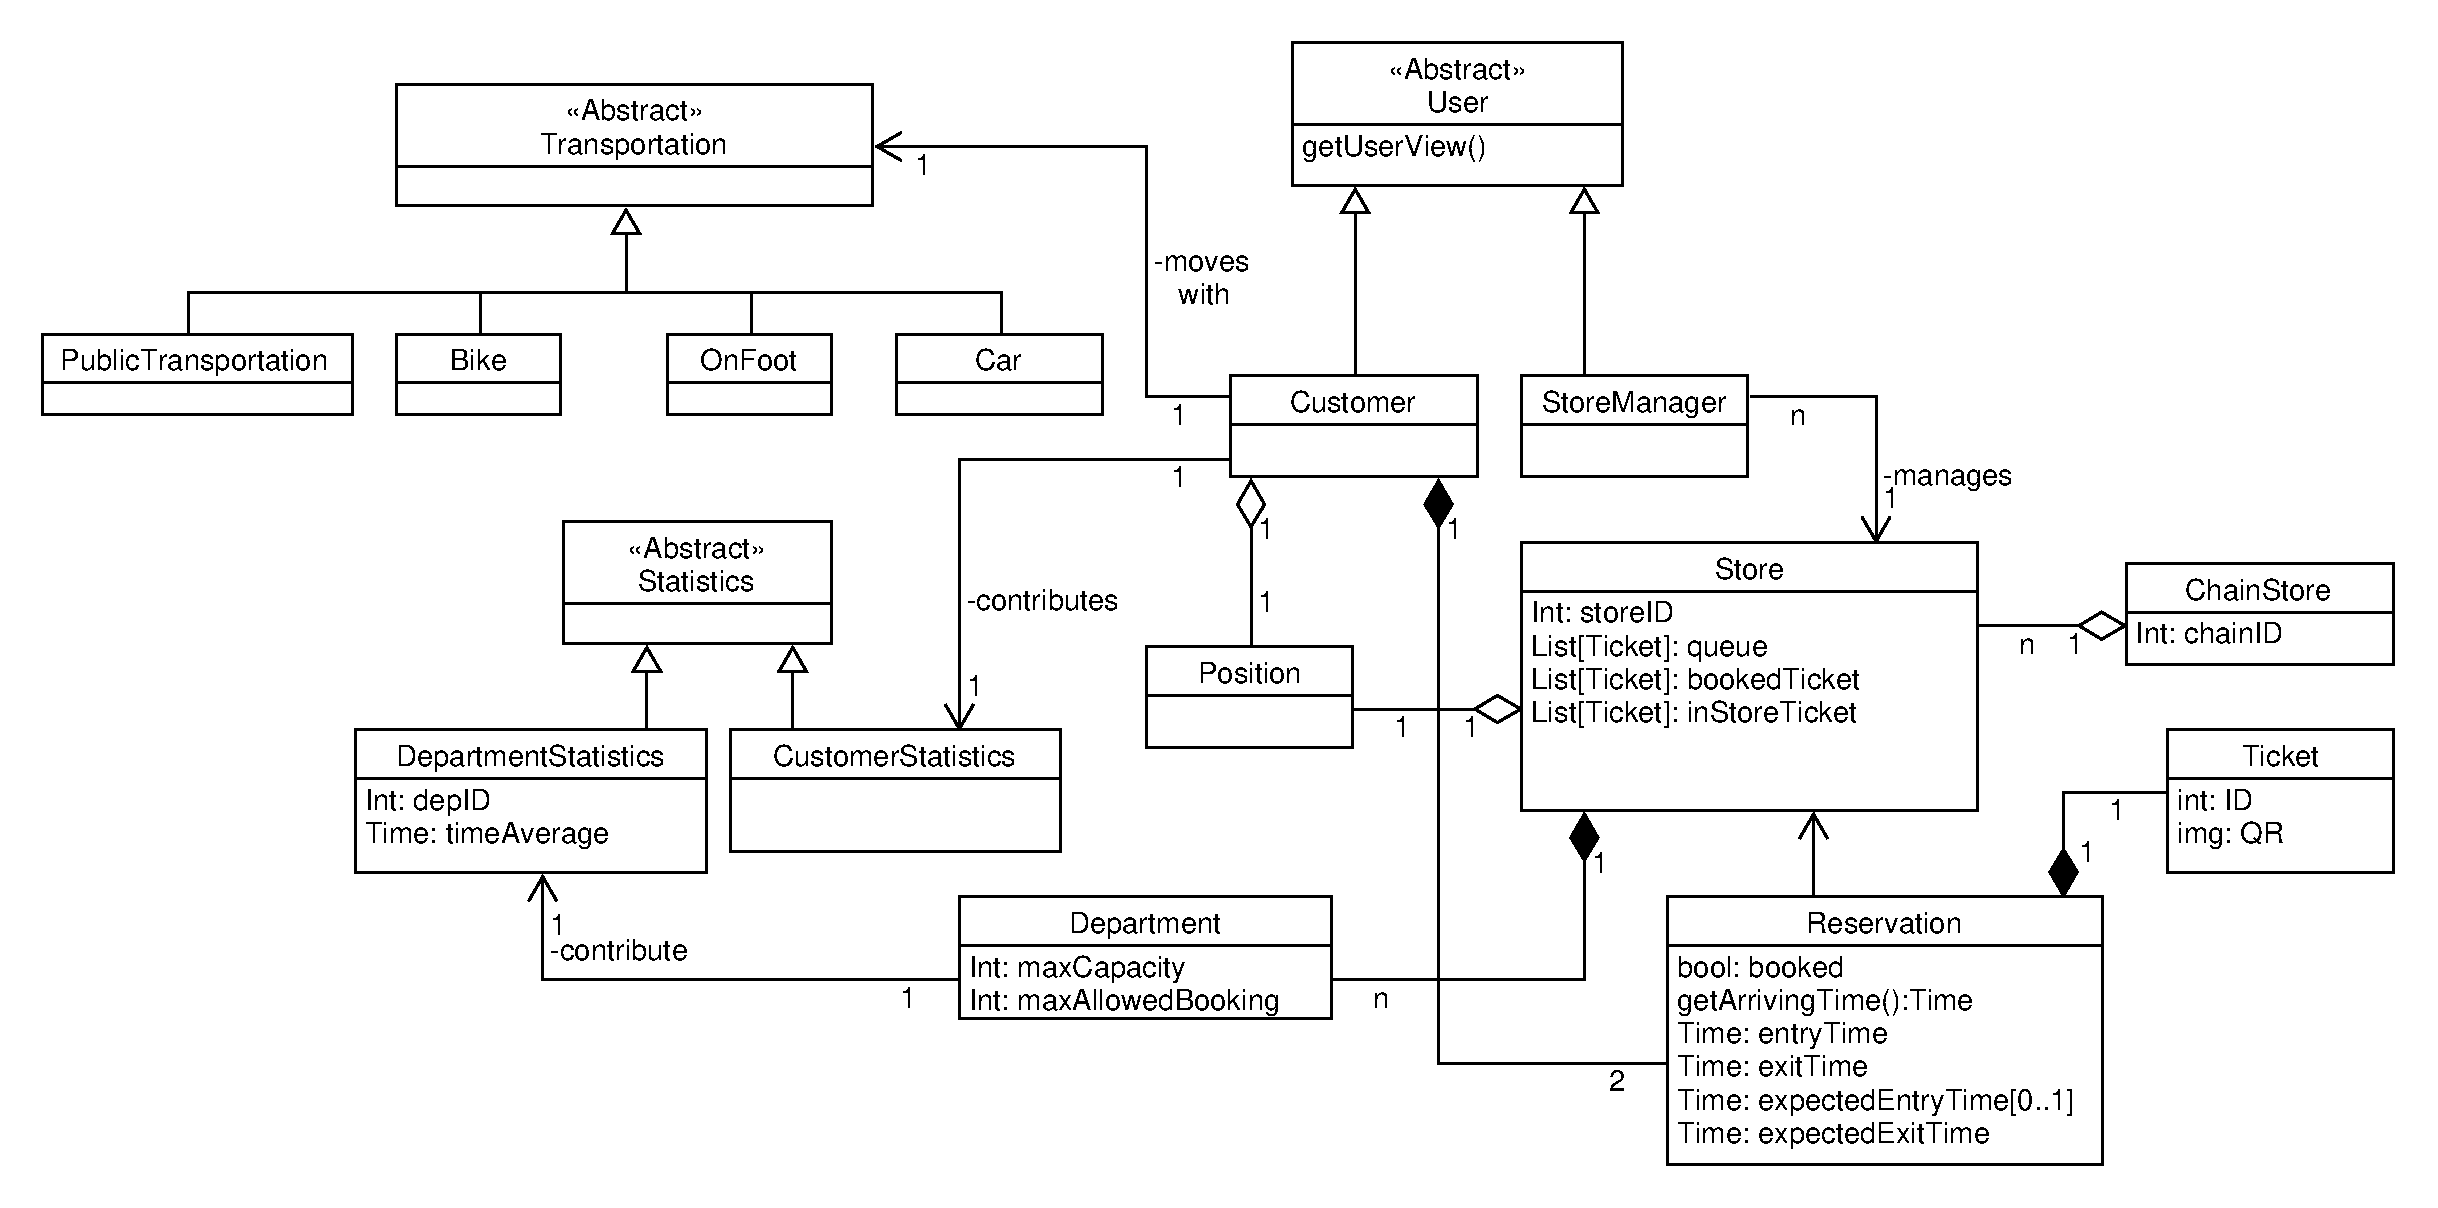
\includegraphics[scale=0.45, angle=90, trim= 0 0 0 -5cm]{ClassDiagrams/classDiagram.pdf} \\
				\caption{\emph{UML Class Diagram}}
			\end{adjustwidth}
		\end{figure}
	
		\newpage
		
		\subsubsection{State Charts}
		
		Now we are going to examine some essential aspects of the application, modelling their behaviours and showing the evolutin over time of their states through adequate state diagrams, which are reported below.
		
		\begin{figure}[!h]
			\centering
			\hspace*{-2.57cm}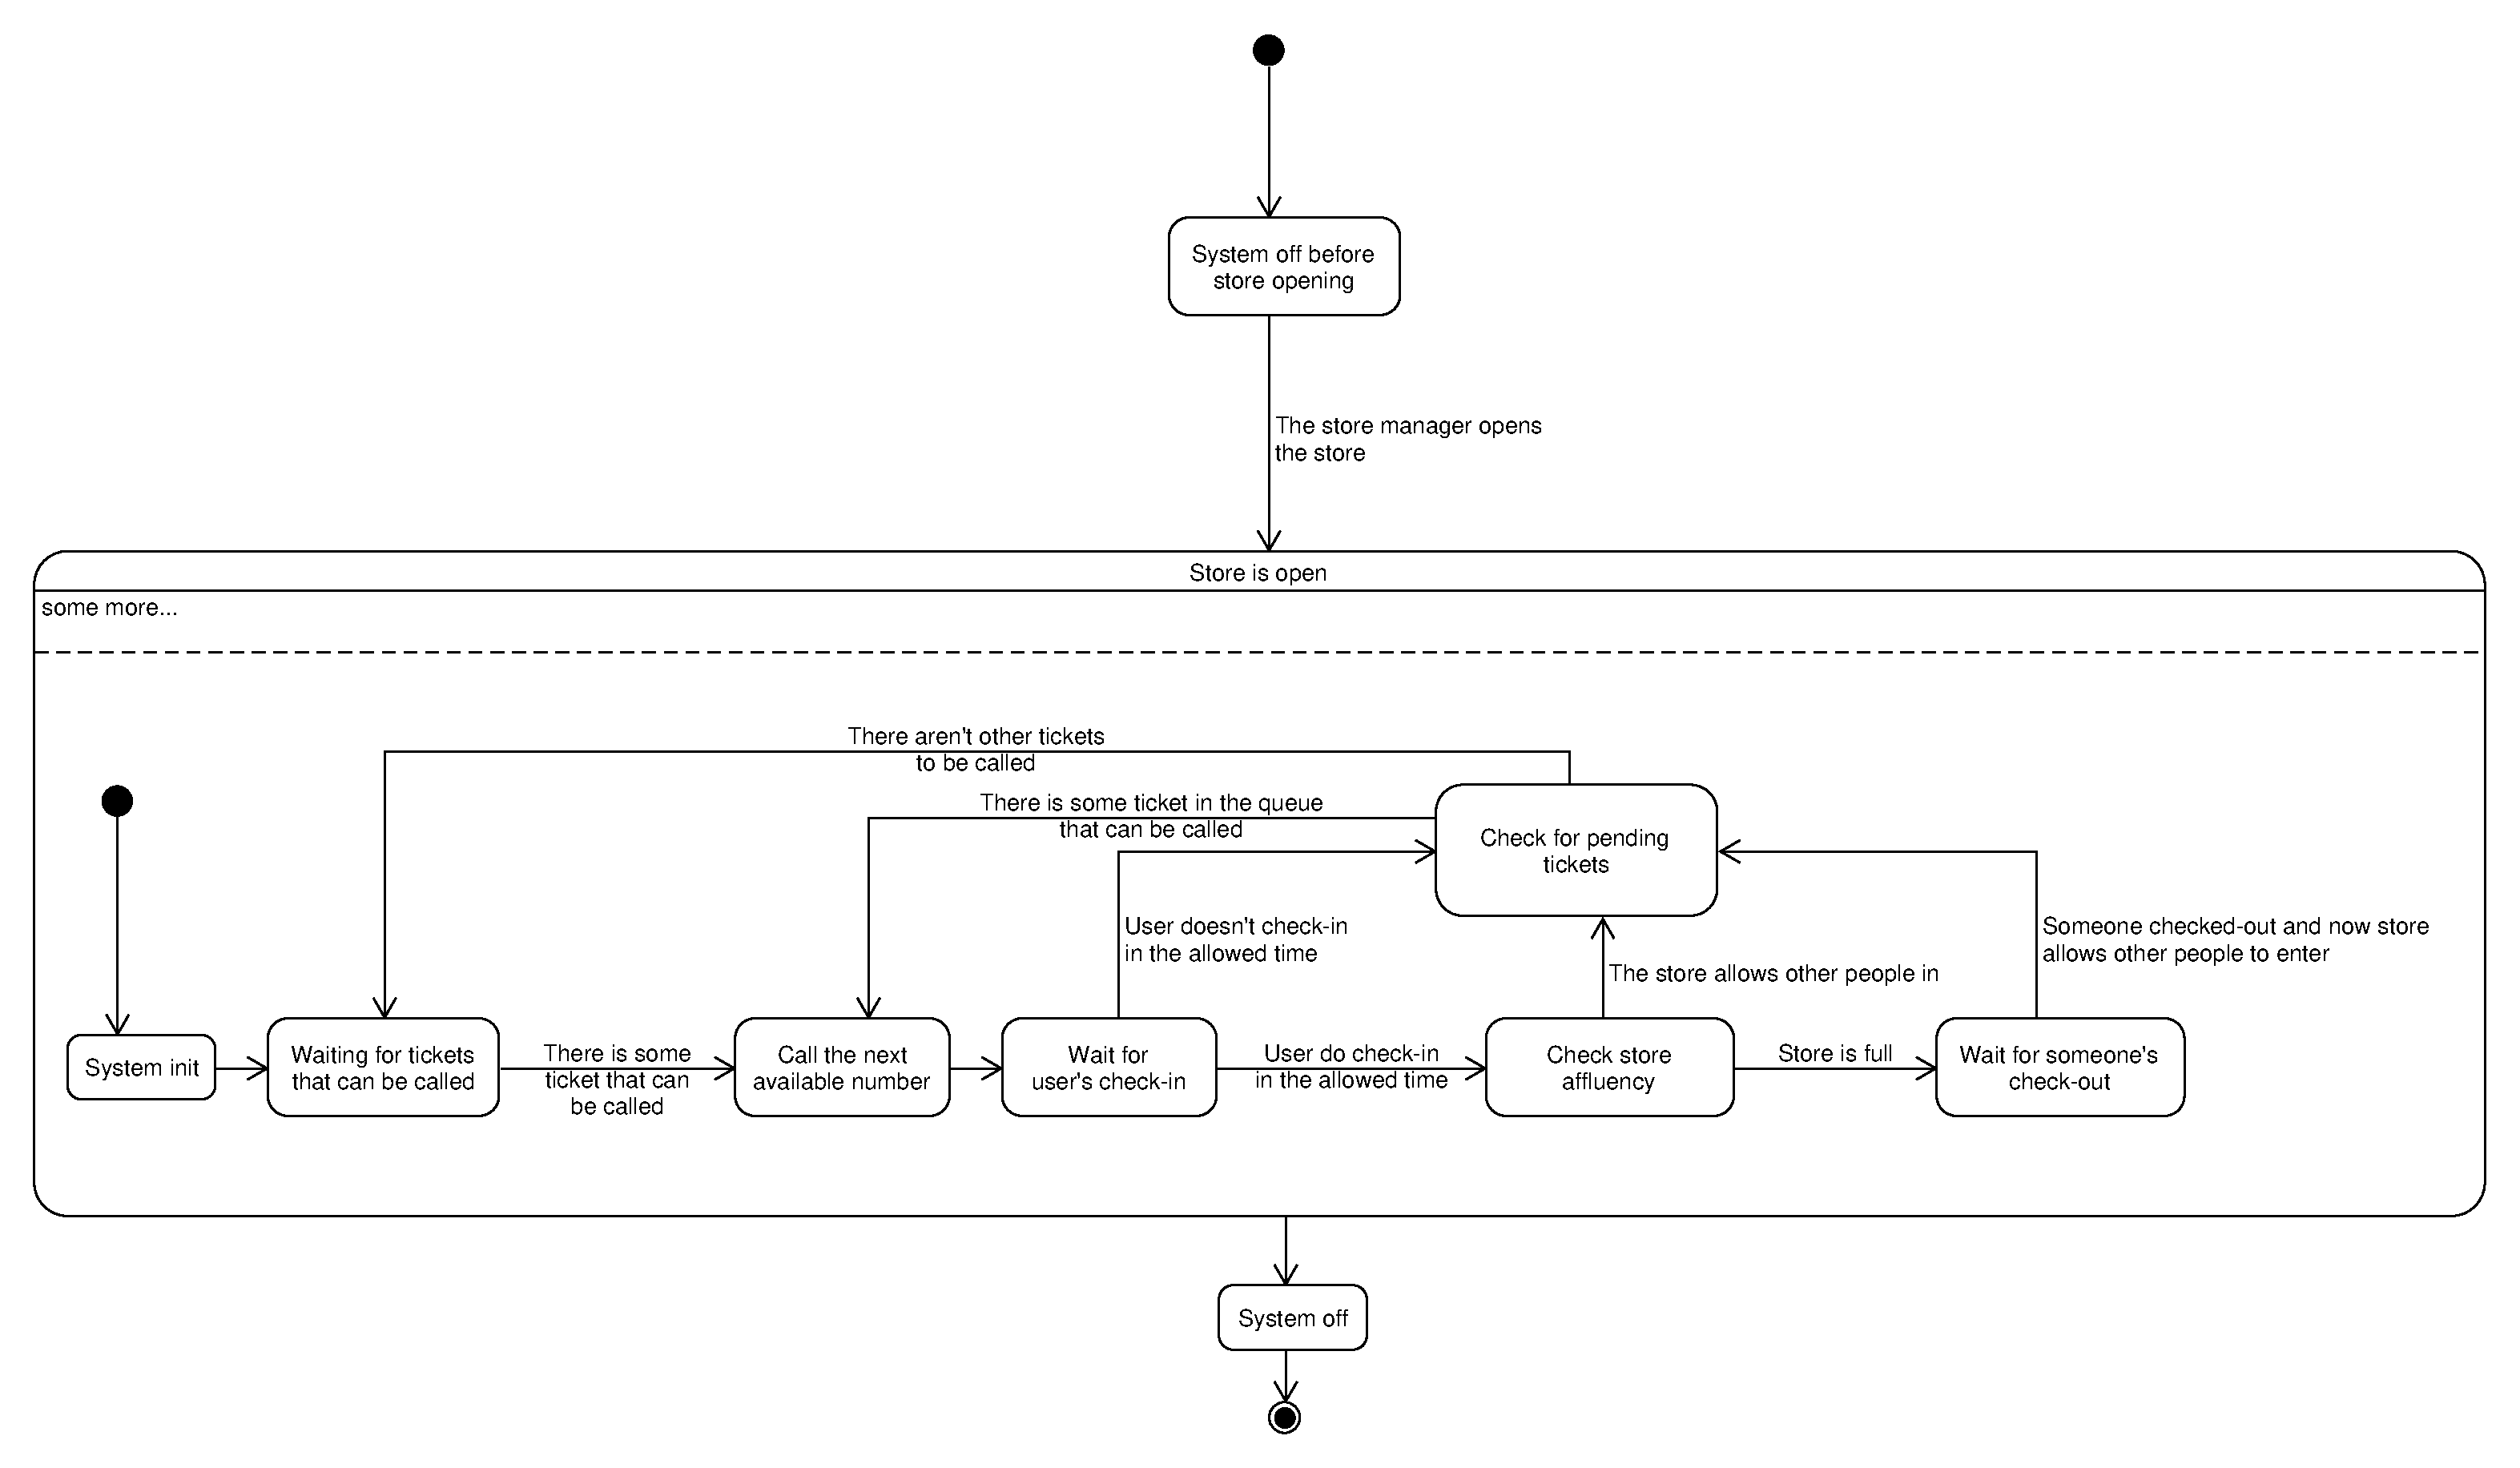
\includegraphics[scale=0.32]{StateCharts/number_calling_system.pdf} \\
			\caption{\emph{Number calling system}}
		\end{figure}
	
		When the store manager opens the store, the system initialize itself and waits for some ticket that can be called. For example, tickets related to the \emph{FIFO} queue can be called as soon as the requested zones are available, and tickets related to bookings can be called only after the start time of the booked time slot, and will be called around this time, when all the booked zones become available (to avoid starvation on calling bookings, other tickets requesting at least one booked zone won't be called until the booked tickets enters the supermarket). After a ticket is available to be called, the system notify in some way (e.g. through a store employee) that now certain ticket is allowed to enter the store. At this point, the system waits for the scan of the associated \emph{QR code}. If the customer doesn't check-in in the assigned time, the system discard the ticket and checks if there are other available tickets. If so, it return in the state of calling the number; else, it will wait for an eligible ticket to be called. If the user, otherwise, scan his \emph{QR code} in time, the system checks the affluence of the store. If it's full, the system will wait for someone's check out, in order to check if some ticket can be called. Else, if the store isn't full, the system doesn't have to wait for a check out to check if there is some ticket eligible to be called. When at some time the store manager will close the store, the system begins its shutdown procedure. It's assumed that at the closure there isn't any other uncalled ticket, since at a certain point the generation of tickets will be blocked, so that that the last ticket will be served around the time of closure.
		
		\bigskip
		
		\begin{figure}[!h]
			
			\centering
			\hspace*{-2cm}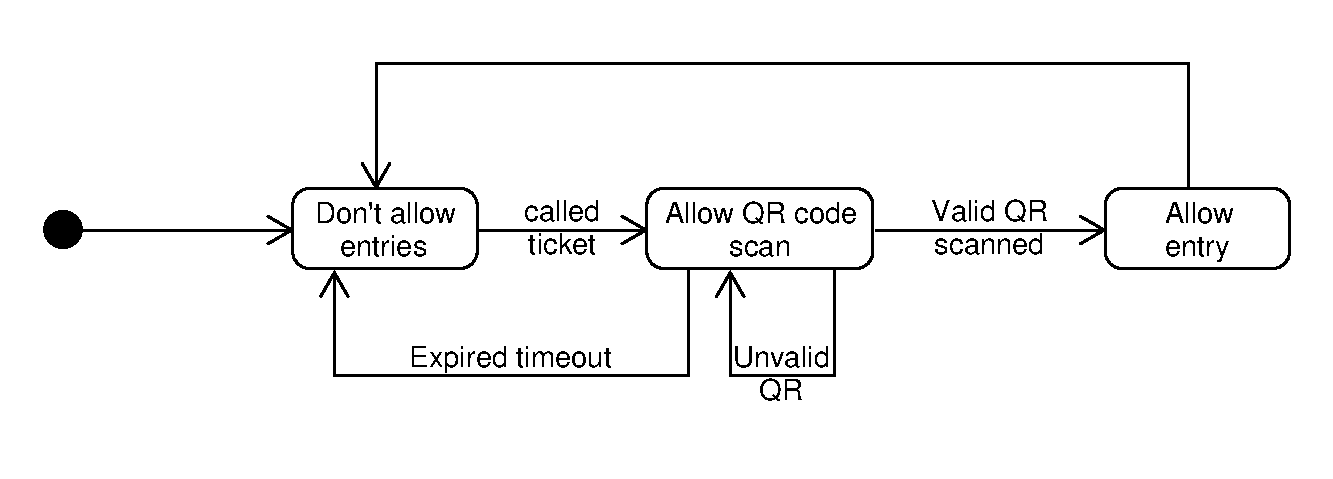
\includegraphics[scale=0.7]{StateCharts/qr_scanner_uml.pdf} \\
			\caption{\emph{QR Code scanner state machine}}
			
		\end{figure}
		
		The system doesn't allow entries since a ticket is called by the system described above. Than, the \emph{QR Code} reader waits for a \emph{QR code} to be scanned. When a \emph{QR Code} is scanned, the system checks if it's a valid one; if so, allows the entry, otherwise notify the wrong \emph{QR Code} and continue waiting for the right one. If the valid \emph{QR Code} isn't scanned in time, the system block the entry and waits for the next called ticket. Otherwise, if the valid \emph{QR Code} is scanned in time, the system allows the entry and, detected the entry, or expired the timeout, block the entries and waits for the next ticket to be called.
		
		\bigskip
		
		To avoid generating tickets that will be called after the closing hour of the store, thanks to the estimations of customers' shopping time, the system is able to decide if it can issue a ticket for entering as soon as possible in the store, or a new ticket's calling time goes over the store opening. After the system detects it can't issue tickets, the ticket generation system blocks ticket issuing until the store is closed, so that the next day the ticket generation can resume.
		\begin{figure}[!h]
	
			\centering
			\hspace*{-2cm}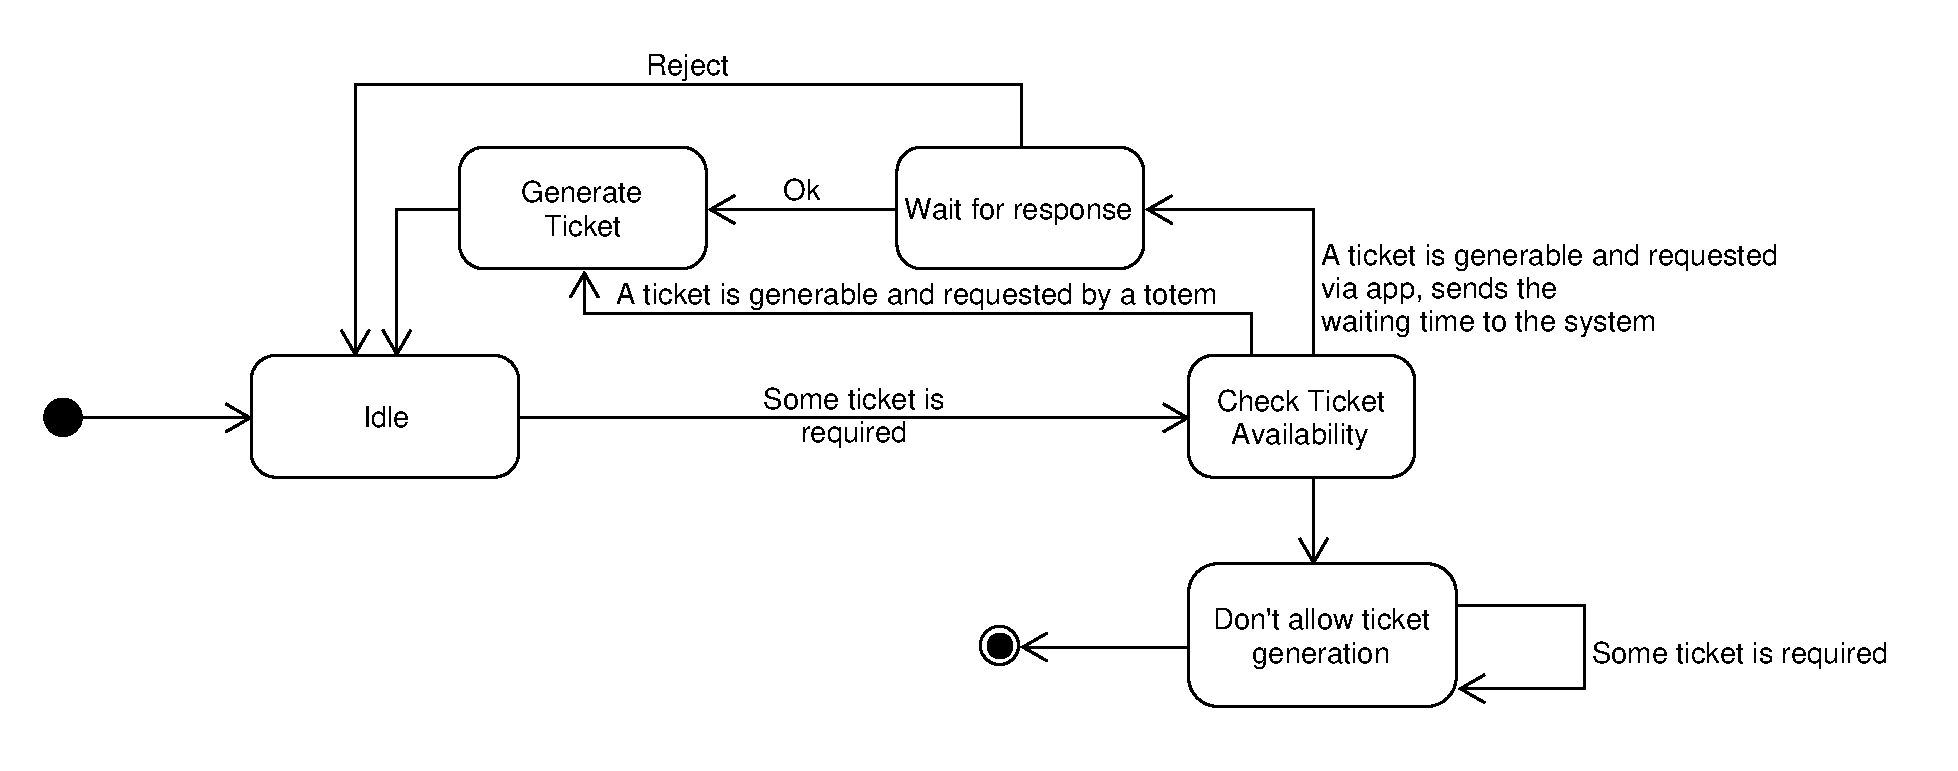
\includegraphics[scale=0.5]{StateCharts/ticket_generator_system.pdf} \\
			\caption{\emph{Ticket generator system state machine}}
	
		\end{figure}
	

	\newpage
	\subsection{Product Functions}
		
	In the previous chapter there were introduced, sketchily, the main features of the software in order to understand, in general, its functioning. Alternatively, in this section will be illustrated and described accurately all the functions that the software allows to do.
	
		\subsubsection{Getting a ticket}
		
		In order to manage the line of the supermarket, it's used a system based on the "call of numbers". Each user in the queque has a unique ID, and when his number is called (eg. by a store employee), the user is authorized to enter. This mechanism works also for the booking feature, since the system generates a number that won't be called until the beginning of the time slot selected by the user. Users can get a ticket both on the application and at a totem installed at the entry of the store (obviously, on the app users are required to select some specific store of their preference from a given list, sorted by the nearest one from the position obtained from the \emph{GPS}). With the generation of the ticket, the user will get both an ID and a \emph{QR Code} associate to it, to be scanned at the enter of the store. When getting a ticket on the application, users must be logged in with their credentials (if not, they must register at the services following the procedure that will be explained later), while at the Totem they can simply get the ticket without giving any data. On app, customers get a digital ticket with its associated \emph{QR Code}; at totem, the ticket and the qr code will be printed. On both of them, there is displayed the expeted time of call. Getting the ticket, the user can indicate the department in which he is interested, and using the app can decide both to have a ticket to enter asap in the store or to plan his visit. At the store's totem, he can only get a ticket to enter as soon as possible. Once completed the operation on the app, the user will be able to see at any moment the time needed to reach the store by the preferred mean of transport selected in the settings.
		
		\subsubsection{Calling process}
		
		The process to admit people in the store follows a \emph{FIFO} logic: the first one that got a ticket, is the first to access the store. When called, a person is authorized to access the store. To register his entry, he is requested to check-in at the entry in a certain amount of time.
		
		\subsubsection{Check-in/Check-out}
		
		At the store entries and exities, users have to scan their \emph{QR Codes} to respectively Check-in and Check-Out in the supermarket. If someones doesn't check-in in a prefixed amount of time, definible by the store manager, he'll lost his turn in the queue. \emph{QR Code} scan is required for two important reasons: register someone's entry in the store for contact tracing purposed, and to check that the person entering the store is the one called, to avoid stoles of turns.
		
		\subsubsection{Plan a visit}
		
		The app allows to brand's customers to plan a visit in a store of their preference. At the end of the process of getting a ticket, if the user select to plan his visit to the store, the software shows the user the time table highlighting the days and the time slots available, in such a way as to allow the user to select the best option for him. If the options do not satisfy the user, he can ask the application for help to find other supermarkets with more comfortable hours. If a reservation process is interrupted in the middle, the user will be able to resume it reopening the app.
		
		\subsubsection{Managing single department}
		
		The system can infer the average time spent by a user in the supermarket using the previous visits as informations. If the client is taking a spot on the queue or booking a visit on the app, he will be asked to insert a reasonable duration of his visit, or let the application to fill this parameter for him: if there aren't enough informations on the specific client, the app will use informations from other clients that did a similar shopping, else will infer the information from the specific client's previous visits. The same thing happens at the totem, where or the client inserts the estimation, or the system will use the other datas in its possession.
		
		\newpage
		
		\subsubsection{Notify users}
		
		If some account have non completed visits, depending on the position of the client (retrieved by \emph{GPS}), and the preferred option of reaching the selected store (eg. on foot, by car or public transport), the app will notify the client when he can exit home, to arrive in time to enter the supermarket, without losing its turn and avoiding long waiting times. Notice that not all of the moving options may be available in all the places, since it depends on the used map service.
		
		\subsubsection{Cancel a visit}
		
		If the user can not reach the store in time, he can decide to cancel the booked visit or the generated ticket. In this case the software delete the customer from the queue and rearrange the last one.
		
		\subsubsection{Store capacity}
		
		The app, also, allows store managers to see the store's affluency and to modify the store capacity in every single repart. When a repart capacity is changed, the already made bookings will be rescheduled at the first available entry time, notifiying each user of the change. The priority is to allow customers that booked the visit to enter in the same day, if it's possible. If any time on the same day can be allocated, the bookings will be cancelled and the user notified. A such operation may reduce in the already booked days the number of admitted non-booked clients. If this operation is made on working hours, it may be cause an anticipation of the time when the system will not deliver anymore other tickets for the queue.
		
		\subsubsection{Infer waiting time from users}
		
		The system can infer the average time spent by a user in the supermarket using the previous visits as informations. If the client is taking a spot on the queue or booking a visit on the app, he will be asked to insert a reasonable duration of his visit, or let the application to fill this parameter for him: if there aren't enough informations on the specific client, the app will use informations from other clients that did a similar shopping, else will infer the information from the specific client's previous visits. The same thing happens at the totem, where or the client inserts the estimation, or the system will use the other datas in its possession.  \\
		
		\newpage
		
		\subsubsection{Allow a fair management of the accesses}
		The system is able to manage in a fair way the process of releasing tickets and accepting bookings. In fact, depending on the store's closing time, and others datas in its possession, such as the number of people in queue, the estimated time of permanency and some other statistics, it's able to block the generation of new tickets, to avoid the generation of turns that goes over the closing time. Moreover, the store manager is able to decide the maximum number of contemporary bookings allowed in the whole store and each department, to avoid that it's really difficult to enter the store without a booking.

	\bigskip
	\subsection{User Characteristics}
	
	\emph{CLup} gives access to two different sets of functionalities based on the two different category of users:
	
	\bigskip
	\begin{itemize}
		
		\item {\bfseries Customer}: Allows user to book a visit to the supermarket. The software generates a \emph{QR Code} that the user can use to enter in the supermarket. The user can indicate the exact list of items that he intends to purchase, or, at least, the categories of items that he intends to buy and, also, he can indicates the approximate expected duration of the visit. Moreover, the user can see the \emph{ETA} to enter the store. \emph{CLup} also allows clients to obtain their book at the store entry.\\
		
		\item {\bfseries Store Manager}: The Store Manager can view information about the store, in particular he can access to the reservations made by users to predict the future affluency and check the level of affluency in the store (and also in specific zones of the store). \\
		
	\end{itemize}

	\subsection{Assumptions, Dependencies, Constraints}
	
	\smallskip
	
		\subsubsection{Domain Assumptions}
		
			\bigskip
			
			\begin{center}
				
				\rowcolors{2}{}{gray!20}
				\rowcolors{1}{gray!20}{white}
				\renewcommand{\arraystretch}{2}
				
				\begin{adjustwidth}{-1.5cm}{}
					\begin{tabular}[h!]{|m{2.5em}|m{32.5em}|}
						
						\hline
						\xrowht{5pt}
						DA1 & Date and time on the devices on which \emph{CLup} runs are always correct \\
						\xrowht{5pt}
						DA2 & Internet connection works always without errors \\
						\xrowht{5pt}
						DA3 & Customer’s position retrieved by \emph{GPS} is accurate \\
						\xrowht{5pt}
						DA4 & In each store, different objects belonging to the same category are in the same department \\
						\xrowht{5pt}
						DA5 & Totems always work properly and are not damaged \\
						\xrowht{5pt}
						DA6 & The customer’s smartphone screen is not damaged and the \emph{QR Code} is readable \\
						\xrowht{5pt}
						DA7 & The \emph{Maps API} always calculate the optimal route \\
						\xrowht{5pt}
						DA8 & Every store has a unique name and address combination \\
						\xrowht{5pt}
						DA9 & \emph{QR Code} readers are always working \\
						\xrowht{5pt}
						DA10 & The store capacity inserted by store manager is always correct \\
						\xrowht{5pt}
						DA11 & Customer respects his time slot, without remaining over time \\
						\xrowht{5pt}
						DA12 & Each customer scans his QR Code at the enter and enters the supermarket only through the allowed entries. \\
						DA13 & Each paper ticket is not ruined and readable. \\
						\hline
						
						
					\end{tabular}
				\end{adjustwidth}
			\end{center}
\newpage

\section{Specific Requirements}

	\subsection{External Interface Requirements}
	
		\subsubsection{User Interfaces}
		
			The user can use the service using a personal mobile device (eg. a smartphone, a smartwatch and a tablet), or through a totem externally installed at each store using CLup to manage the access of clients. Store managers can also use a personal mobile device to manage the store. In this section we’ll present the general mockups relative to the smartphone version of both customer and manager management, since it is the landmark for the development of the entire system.
		
		\subsubsection{Hardware Interfaces}
		
			The managers’ side of the application doesn’t require any special hardware requirement except for a network module installed in their device, since all of the information required is already stored in the system. Clients’ side, anyways, requires a working GPS module, a working network module and a not broken display to scan the generated QR Code at the store entry. Instead, at the store we need: a device with a ticket printer and a working network module to generate and print tickets, some (at least one for entry and one for exit) optical scanners to scan QR Codes, and another device with a working network module to manage ticket calling.
			
			
		\subsubsection{Software Interfaces}
		
			The system can send notification to the customer with regard to notify him to depart in time for reach the store and to avoid losing his turn in lineup. To do this, the system uses a public API to provide customer his exact position and, so, calculate the optimal route from customer's position to the store. The exact position is also used to sort by distance the list of bookable store. Moreover, the system permits to store manager to communicate with customers in case of a reservation must be deleted or postponed for every reason.
			
		\subsubsection{Communication Interfaces}
		
			It is necessary to develop a communication interface in order to allow the different systems to communicate one to each other, achieving the integration of the store’s side and of the user’s side.
	\newpage
	\subsection{Functional Requirements}
	
		\subsubsection{List of Requirements}
		
			\begin{center}
				
				\setlength\LTleft{-50pt}
				
				\rowcolors{2}{}{gray!20}
				\rowcolors{1}{gray!20}{white}
				\renewcommand{\arraystretch}{2}
				
				\begin{adjustwidth}{-1.5cm}{}
					\begin{longtable}[h!]{|m{2.5em}|m{32.5em}|}
						
						\hline
						\xrowht{5pt}
						R1 & The system must allow the customers to register \\
						\xrowht{5pt}
						R2 & The system must allow store managers to register their store \\
						\xrowht{5pt}
						R3 & The system must allow customers to log in \\
						\xrowht{5pt}
						R4 & The system must allow store managers to log in \\
						\xrowht{5pt}
						R5 & The system allows the customers to view their visits \\
						\xrowht{5pt}
						R6 & The system allows the customers to cancel their visits \\
						\xrowht{5pt}
						R7 & The system allows the customers to modify their visits \\
						\xrowht{5pt}
						R8 & The system allows the customers to select their favorite means of transportation \\
						\xrowht{5pt}
						R9 & The system allows the customers to select some or all the departments in which the customers are interested in doing shopping \\
						\xrowht{5pt}
						R10 & The system must let in customers only if is their turn \\
						\xrowht{5pt}
						R11 & The system must consider the extimate shopping time insert by customers \\
						\xrowht{5pt}
						R12 & The system must show the customers of the time periods in which they can enter the store in order to respect the time selected by the customers \\
						\xrowht{5pt}
						R13 & The system have to make a reasonable estimate of when a user with a spot on the queue is able to enter the store \\
						\xrowht{5pt}
						R14 & The system can send notification to the clients \\
						\xrowht{5pt}
						R15 & The system is able to ask for the position of the customers \\
						\xrowht{5pt}
						R16 & The system permits to store manager to modify the maximum capacity of the store's departments  \\
						\xrowht{5pt}
						R17 & The system permits to store manager to view the statistics of the store and its departments \\
						\hline
						\hline
						\xrowht{5pt}
						R18 & The system allows the manager to establish the maximum simultaneously
						allowed booked clients in a specific department \\
						\xrowht{5pt}
						R19 & The store manager can view the reservation of each client \\
						\xrowht{5pt}
						R20 & The store manager can modify the reservation of each client \\
						\xrowht{5pt}
						R21 & The store manager can cancel the reservation of each client \\
						\xrowht{5pt}
						R22 & The store manager can handle the opening and closing time of the store \\
						\xrowht{5pt}
						R23 & The system knows the situation in real time of each store \\
						\xrowht{5pt}
						R24 & The system takes trace of each customer entry and exit from the store \\
						\xrowht{5pt}
						R25 & The system contains a list of bookable stores \\
						\xrowht{5pt}
						R26 & The systemis able to print a paper ticket \\
						\xrowht{5pt}
						R27 & The system can reasonably estimate the time needed from a specific user to complete his shopping \\
						\xrowht{5pt}
						R28 & The system must save clients’ tickets \\
						\xrowht{5pt}
						R29 & The system should estimate when it must stop generating other tickets to avoid turns after the closing time of the store \\
						R30 & The system is able to smartly call clients with a ticket to enter the building depending on reservations and people inside the building \\
						R31 & The system is able to scan and analyze a QR Code \\
						R32 & The system is able to send emails \\
						\hline
						
					\end{longtable}
				\end{adjustwidth}
			\end{center}
		
		\newpage
		
		\subsubsection{Mapping with goals}
			
			\begin{itemize}			

				\item {\bfseries G1: Allow customers to select a store and book a spot on the queue from CLup app}			

					\begin{itemize}
						
						\item {\bfseries R1}: The system must allow the customers to register
						\item {\bfseries R2}: The system must allow customers to log in
						\item {\bfseries R9}: The system allows the customers to select some or all the departments in which the customers are interested in doing shopping						\item {\bfseries R11}: The system must consider the extimate shopping time insert by customers
						\item {\bfseries R12}: The system must show the customers of the time periods in which they can enter the store in order to respect the time selected by the customers
						\item {\bfseries R13}: The system have to make a reasonable estimate of when a user with a spot on the queue is able to enter the store
						\item {\bfseries R15}: The system is able to ask for the position of the customers
						\item {\bfseries R23}: The system knows the situation in real time of each store \\				\item {\bfseries R25}: The system contains a list of bookable stores
						\item {\bfseries R27}: The system can reasonably estimate the time needed from a specific user to complete his shopping
						\item {\bfseries R28}: The system must save clients’ tickets
						
						
						\item {\bfseries DA1}: Date and time on the devices on which CLup runs are always correct
						\item {\bfseries DA2}: Internet connection works always without errors
						\item {\bfseries DA3}: Customer’s position retrieved by GPS is accurate
						\item {\bfseries DA8}: Every store has a unique name and address combination
					
					\end{itemize}
				
				\item {\bfseries G2: Allow customers to select a store and take a spot on the queue to enter as soon as possible the store from CLup app}	

					\begin{itemize}
						
						\item {\bfseries R1}: The system must allow the customers to register
						\item {\bfseries R2}: The system must allow customers to log inn
						\item {\bfseries R9}: The system allows the customers to select some or all the departments in which the customers are interested in doing shopping							\item {\bfseries R11}: The system must consider the extimate shopping time insert by customers
						\item {\bfseries R15}: The system is able to ask for the position of the customers
						\item {\bfseries R23}: The system knows the situation in real time of each store
						\item {\bfseries R25}: The system contains a list of bookable stores
						\item {\bfseries R27}: The system can reasonably estimate the time needed from a specific user to complete his shopping
						\item {\bfseries R28}: The system must save clients’ tickets
						\item {\bfseries R29}: The system should estimate when it must stop generating other tickets to avoid turns after the closing time of the store \\
		
						\item {\bfseries DA1}: Date and time on the devices on which CLup runs are always correct
						\item {\bfseries DA2}: Internet connection works always without errors
						\item {\bfseries DA3}: Customer’s position retrieved by GPS is accurate
						\item {\bfseries DA8}: Every store has a unique name and address combination
						
					\end{itemize}

				\item {\bfseries G3: Allow customers to take a spot on the queue from a physical ticket dispenser}	

					\begin{itemize}
						
						\item {\bfseries R9}: The system allows the customers to select some or all the departments in which the customers are interested in doing shopping
						\item {\bfseries R11}: The system must consider the extimate shopping time insert by customers
						\item {\bfseries R13}: The system have to make a reasonable estimate of when a user with a spot on the queue is able to enter the store
						\item {\bfseries R26}: The system is able to print a paper ticket
						\item {\bfseries R27}: The system can reasonably estimate the time needed from a specific user to complete his shopping
						\item {\bfseries R28}: The system must save clients’ tickets
						\item {\bfseries R29}: The system should estimate when it must stop generating other tickets to	avoid turns after the closing time of the store \\
		
						\item {\bfseries DA1}: Date and time on the devices on which CLup runs are always correct
						\item {\bfseries DA2}: Internet connection works always without errors
						\item {\bfseries DA5}: Totems always work properly and are not damaged
						
					\end{itemize}

				\item {\bfseries G4: Allow customers to select a better store option to avoid wasting a lot of time waiting to enter a specific store.}	

					\begin{itemize}
						
						\item {\bfseries R1}: The system must allow the customers to register
						\item {\bfseries R2}: The system must allow customers to log in
						\item {\bfseries R8}: The system allows the customers to select their favorite means of transportation
						\item {\bfseries R13}: The system have to make a reasonable estimate of when a user with a spot on the queue is able to enter the store
						\item {\bfseries R15}: The system is able to ask for the position of the customers
						\item {\bfseries R23}: The system knows the situation in real time of each store
						\item {\bfseries R25}: The system contains a list of bookable stores
						\item {\bfseries R29}: The system should estimate when it must stop generating other tickets to	avoid turns after the closing time of the store \\
		
						\item {\bfseries DA1}: Date and time on the devices on which CLup runs are always correct
						\item {\bfseries DA2}: Internet connection works always without errors
						\item {\bfseries DA3}: Customer’s position retrieved by GPS is accurate
						\item {\bfseries DA7}: The Maps API always calculate the optimal route 
						\item {\bfseries DA8}: Every store has a unique name and address combination
						
					\end{itemize}

				\item {\bfseries G5: Allow customers to decrease waiting times specifying departments they want to visit}	

					\begin{itemize}
						
						\item {\bfseries R1}: The system must allow the customers to register
						\item {\bfseries R2}: The system must allow customers to log in
						\item {\bfseries R9}: The system allows the customers to select some or all the departments in which the customers are interested in doing shopping
						\item {\bfseries R11}: The system must consider the extimate shopping time insert by customers

						\item {\bfseries R13}: The system have to make a reasonable estimate of when a user with a spot on the queue is able to enter the store
						\item {\bfseries R24}: The system takes trace of each customer entry and exit from the store
						\item {\bfseries R27}: The system can reasonably estimate the time needed from a specific user to complete his shopping \\
		
						\item {\bfseries DA1}: Date and time on the devices on which CLup runs are always correct
						\item {\bfseries DA2}: Internet connection works always without errors
						
					\end{itemize}

				\item {\bfseries G6: Allow customers users to manage their spots on the queue and their reservation}	

					\begin{itemize}
						\item {\bfseries R1}: The system must allow the customers to register
						\item {\bfseries R2}: The system must allow customers to log in
						\item {\bfseries R5}: The system allows the customers to view their visits
						\item {\bfseries R6}: The system allows the customers to cancel their visits
						\item {\bfseries R7}: The system allows the customers to modify their visits
						\item {\bfseries R28}: The system must save clients’ tickets \\
		
						\item {\bfseries DA1}: Date and time on the devices on which CLup runs are always correct
						\item {\bfseries DA2}: Internet connection works always without errors
							
					\end{itemize}

				 
				
				\item {\bfseries G7: Allow customers to depart from their location in time to avoid waiting too much, and to avoid losing their turn in lineup}	

					\begin{itemize}
						\item {\bfseries R1}: The system must allow the customers to register
						\item {\bfseries R2}: The system must allow customers to log in
						\item {\bfseries R8}: The system allows the customers to select their favorite means of transportation
						\item {\bfseries R9}: The system allows the customers to select some or all the departments in which the customers are interested in doing shopping
						\item {\bfseries R11}: The system must consider the extimate shopping time insert by customers
						\item {\bfseries R13}: The system have to make a reasonable estimate of when a user with a spot on the queue is able to enter the store
						\item {\bfseries R14}: The system can send notification to the clients
						\item {\bfseries R15}: The system is able to ask for the position of the customers
						\item {\bfseries R24}: The system takes trace of each customer entry and exit from the store
						\item {\bfseries R27}: The system can reasonably estimate the time needed from a specific user to complete his shopping
						\item {\bfseries R28}: The system must save clients’ tickets \\
					
						\item {\bfseries DA1}: Date and time on the devices on which CLup runs are always correct
						\item {\bfseries DA2}: Internet connection works always without errors
						\item {\bfseries DA7}: The Maps API always calculate the optimal route 
						\item {\bfseries DA8}: Every store has a unique name and address combination
							
					\end{itemize}	

				\item {\bfseries G8: Allow store managers to decide how many people, and how many simultaneous booked clients to have in the store and in which department}	

					\begin{itemize}
						
						\item {\bfseries R2}: The system must allow store managers to register their store
						\item {\bfseries R4}: The system must allow store managers to log in
						\item {\bfseries R14}: The system can send notification to the clients
						\item {\bfseries R16}: The system permits to store manager to modify the maximum capacity of the store's departments 
						\item {\bfseries R18}: The system allows the manager to establish the maximum simultaneously allowed booked clients in a specific department
						\item {\bfseries R22}: The store manager can handle the opening and closing time of the store
						\item {\bfseries R28}: The system must save clients’ tickets \\
		
						\item {\bfseries DA1}: Date and time on the devices on which CLup runs are always correct
						\item {\bfseries DA2}: Internet connection works always without errors
						
					\end{itemize}	

				\item {\bfseries G9: Allow the store manager to know the real situation of people that are inside the building and in which department of his store}	

					\begin{itemize}
						
						\item {\bfseries R2}: The system must allow store managers to register their store
						\item {\bfseries R4}: The system must allow store managers to log in
						\item {\bfseries R17}: The system permits to store manager to view the statistics of the store and its departments
						\item {\bfseries R24}: The system takes trace of each customer entry and exit from the store
						\item {\bfseries R31}: The system is able to scan and analyze a QR Code \\		
				
						\item {\bfseries DA1}: Date and time on the devices on which CLup runs are always correct
						\item {\bfseries DA2}: Internet connection works always without errors
						\item {\bfseries DA9}: QR Code readers are always working
						\item {\bfseries DA12}: Each customer scans his QR Code at the enter and enters the supermarket only through the allowed entries.
							
					\end{itemize}

				\item {\bfseries G10: Allow to grant a fair management of users that can access the building.}	

					\begin{itemize}
						
						\item {\bfseries R2}: The system must allow store managers to register their store
						\item {\bfseries R4}: The system must allow store managers to log in
						\item {\bfseries R10}: The system must let in customers only if is their turn
						\item {\bfseries R18}: The system allows the manager to establish the maximum simultaneously allowed booked clients in a specific department
						\item {\bfseries R22}: The store manager can handle the opening and closing time of the store
						\item {\bfseries R29}: The system should estimate when it must stop generating other tickets to avoid turns after the closing time of the store \\
						
						\item {\bfseries DA1}: Date and time on the devices on which CLup runs are always correct
						\item {\bfseries DA2}: Internet connection works always without errors
					
					\end{itemize}
				
				\item {\bfseries G11: Allow to manage optimally the influx in the building and avoid gathering inside it}	

					\begin{itemize}
						
						\item {\bfseries R10}: The system must let in customers only if it's their turn
						\item {\bfseries R24}: The system takes trace of each customer entry and exit from the store
						\item {\bfseries R27}: The system must save clients’ tickets				
						\item {\bfseries R30}: The system is able to smartly call clients with a ticket to enter the building depending on reservations and people inside the building
						\item {\bfseries R31}: The system is able to scan and analyze a QR Code \\
		
						\item {\bfseries DA1}: Date and time on the devices on which CLup runs are always correct
						\item {\bfseries DA2}: Internet connection works always without errors
						\item {\bfseries DA9}: QR Code readers are always working
						\item{\bfseries DA6}: The customer’s smartphone screen is not damaged and the QR Code is readable
						\item {\bfseries DA12}: Each customer scans his QR Code at the enter and enters the supermarket only through the allowed entries
						\item {\bfseries DA13:} Each paper ticket is not ruined and readable
					
					\end{itemize}

				\item {\bfseries G12: Allow the store manager to manage customers’ bookings}	

					\begin{itemize}
						\item {\bfseries R2}: The system must allow store managers to register their store
						\item {\bfseries R4}: The system must allow store managers to log in
						\item {\bfseries R19}: The store manager can cancel the reservation of each client
						\item {\bfseries R20}: The store manager can modify the reservation of each client
						\item {\bfseries R21}: The store manager can view the reservation of each client
						\item {\bfseries R27}: The system must save clients’ tickets \\
		
						\item {\bfseries DA1}: Date and time on the devices on which CLup runs are always correct
						\item {\bfseries DA2}: Internet connection works always without errors
						\newpage
		
					\end{itemize}

			\end{itemize}

		\subsubsection{Use Cases}
		

			
			\paragraph{Registration of a customer}
			
				\begin{center}
					
					\rowcolors{2}{}{gray!20}
					\rowcolors{1}{gray!20}{white}
					
					\begin{adjustwidth}{-2.8cm}{}
					\begin{tabular}[h!]{|m{7.5em}|m{36em}|}
						
						\hline
						\xrowht{5pt}
						Name &  Registration of a customer\\
						\xrowht{5pt}
						Actors & Customer\\
						\xrowht{5pt}
						Entry Condition & Customer has the internet connection available and has accessed the application on its device\\
						\xrowht{5pt}
						Event Flow & \begin{enumerate}
							
							\itemsep-0.25em
							\item Customer visualizes the initial page of the app
							\item Customer clicks on “Sign up as customer” button
							\item Customer inserts a username, a password, an e-mail, his name, his surname and his phone number as mandatory fields
							\item The system checks the datas of the customer
							\item The system saves the information of the customer
						
						\end{enumerate}\\
						\xrowht{5pt}
						Exit Conditions & Customer is successfully registered to the application\\
						\xrowht{5pt}
						Exception & \begin{enumerate}
							
							\itemsep-0.25em
							\item The username is already present in the system
							\item The customer did not fill up all the mandatory fields with valid data
						
						\end{enumerate}
						If one or more of the above situations occur, the application will throw an error message and will return to the registration form page\\		
						\hline
						
					\end{tabular}

					
					

					\begin{figure}[!h]
						\begin{adjustwidth} {-1cm}{}
							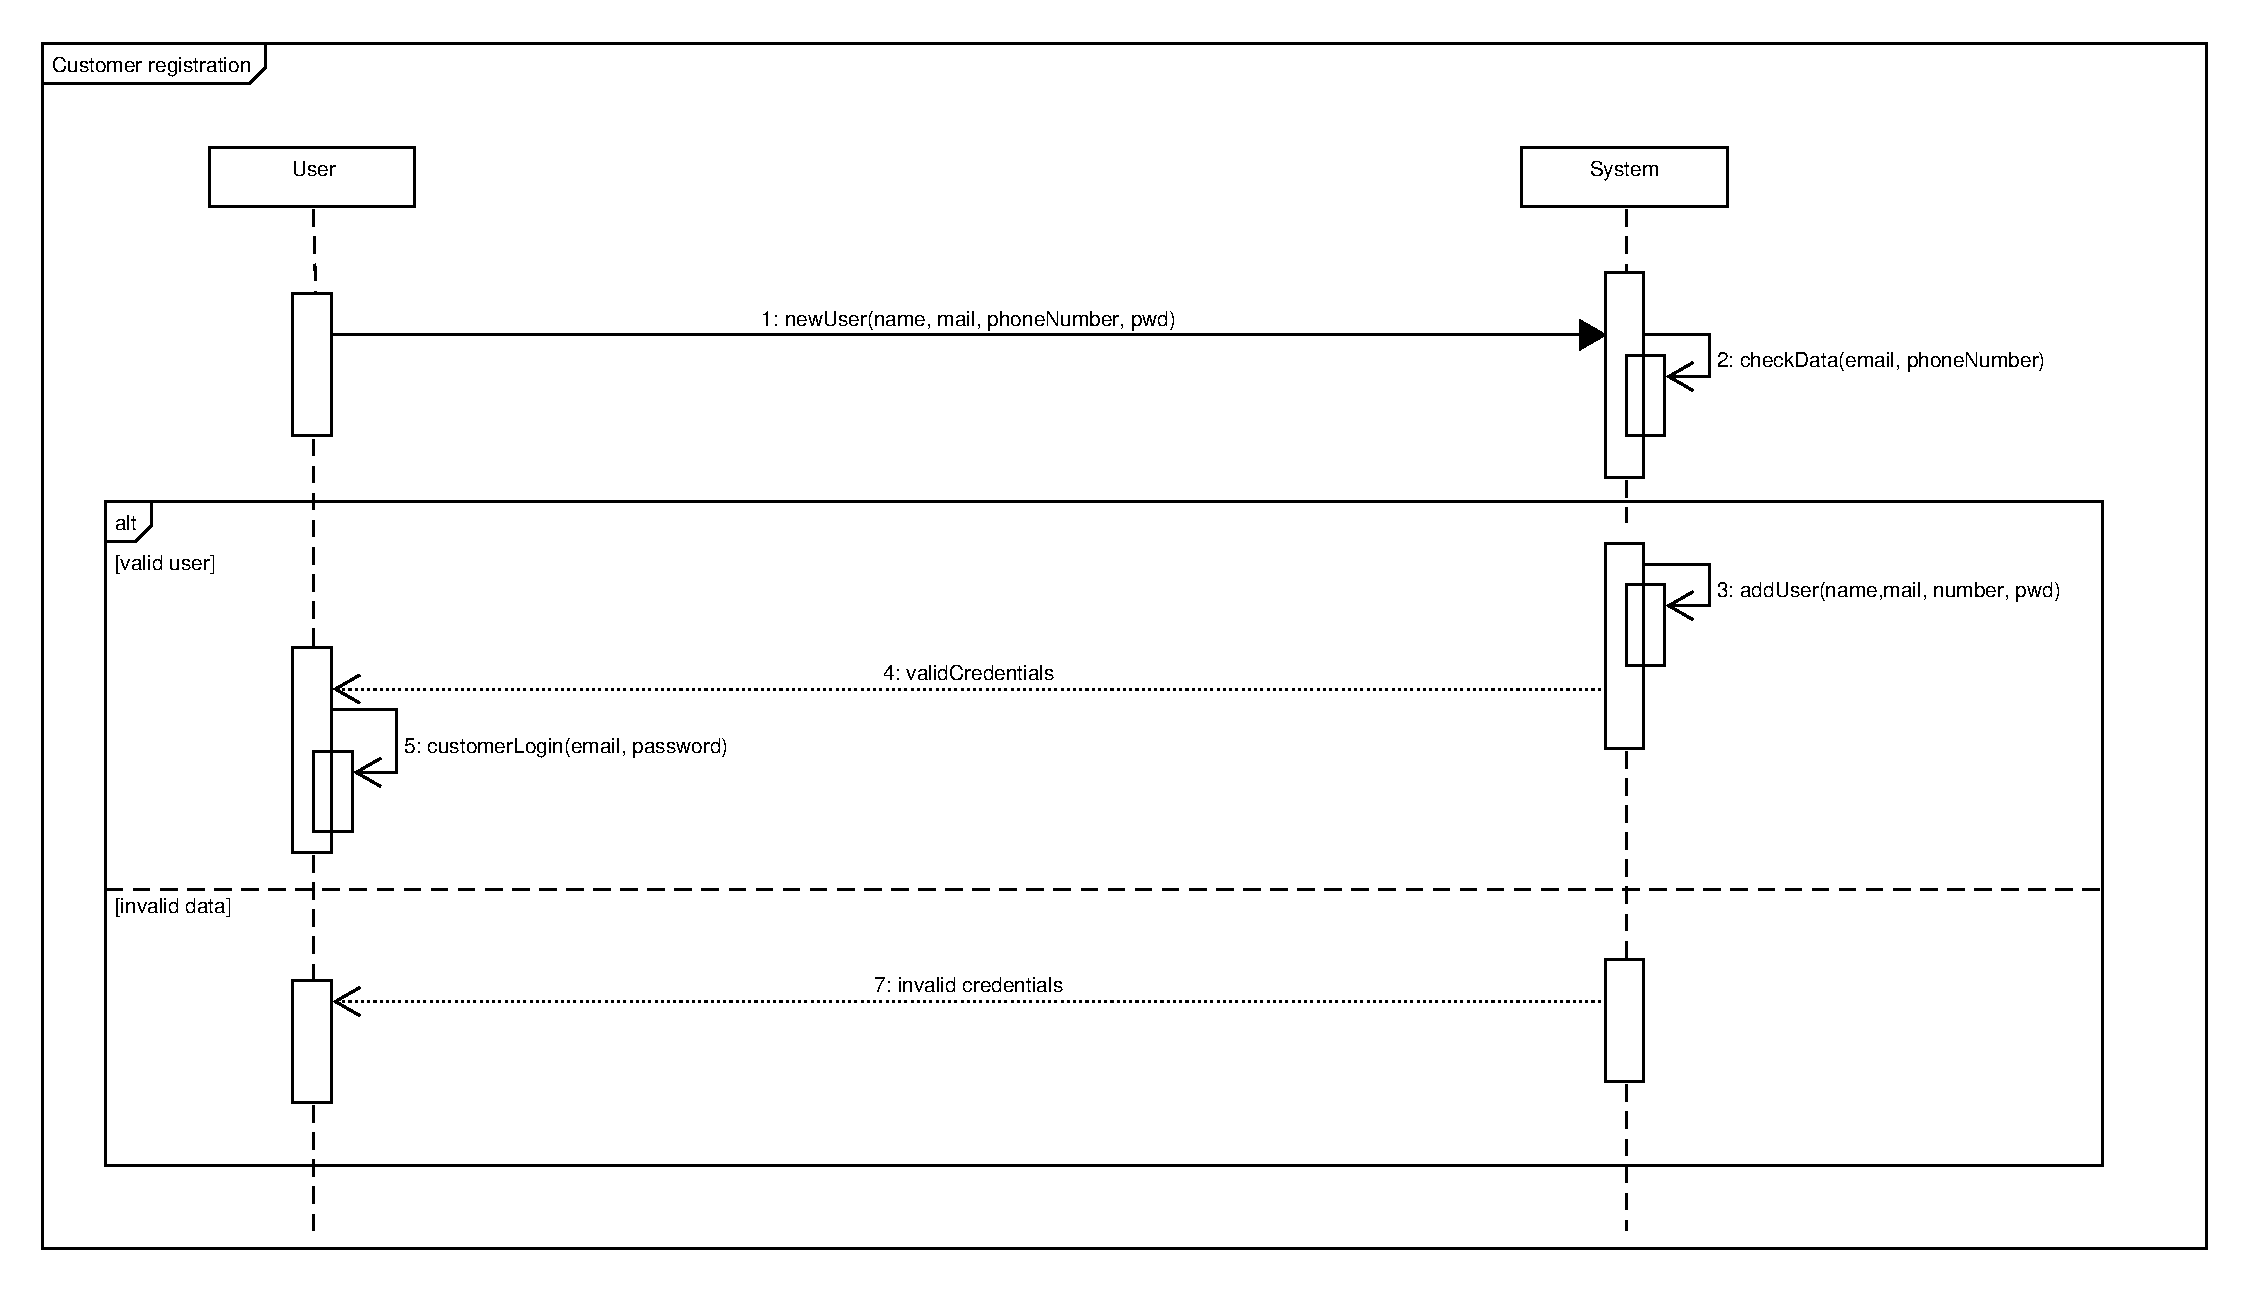
\includegraphics[scale=0.36]{SD/1_customerRegistration.pdf}
						\end{adjustwidth}
						\caption{Sequence Diagram of User Registration}
					\end{figure}

					

					\end{adjustwidth}
					\begin{itemize}
					\medskip
					 {\bfseries Required functional requirements: }
					\item {\bfseries R1: } The system must allow the customers to register


					\end{itemize}
				\end{center}
		\bigskip
			\paragraph{Registration of a store}
			
				\begin{center}
					
					\rowcolors{2}{}{gray!20}
					\rowcolors{1}{gray!20}{white}
					
					\begin{adjustwidth}{-2.8cm}{}
					\begin{tabular}[h!]{|m{7.5em}|m{36em}|}
						
						\hline
						\xrowht{5pt}
						Name & Registration of a store\\
						\xrowht{5pt}
						Actors & Store manager\\
						\xrowht{5pt}
						Entry Condition & Store manager has the internet connection available and has accessed the application on its device\\
						\xrowht{5pt}
						Event Flow & \begin{enumerate}
							
							\itemsep-0.25em
							\item Store manager visualizes the initial page of the app
							\item Store manager clicks on “Sign up as store” button
							\item Store manager compile all the mandatory fields concerning the store
							\item Store manager loads a certification document which proves that it is a real store
							\item The system validates the certification
							\item The system confirms the registration of the store
							\item The system saves the information of the store
							
						\end{enumerate}\\
						\xrowht{5pt}
						Exit Conditions & The store is successfully registered to the application\\
						\xrowht{5pt}
						Exception & \begin{enumerate}
							
							\itemsep-0.25em
							\item The store is already present in the system
							\item The store manager did not fill up all the mandatory fields with valid data
							\item The certification is invalid
							
						\end{enumerate}
						If one or more of the above situations occur, the application will throw an error message and will return to the registration form page\\		
						\hline
						
					\end{tabular}
					\end{adjustwidth}
					
					\begin{itemize}
					\bigskip
					\bigskip
					\bigskip
					 {\bfseries Required functional requirements: }
					\item {\bfseries R2: } The system must allow store managers to register their store

					\end{itemize}
				
					
						
							\begin{figure}
								\begin{adjustwidth} {-2.3cm}{}
									\centering
									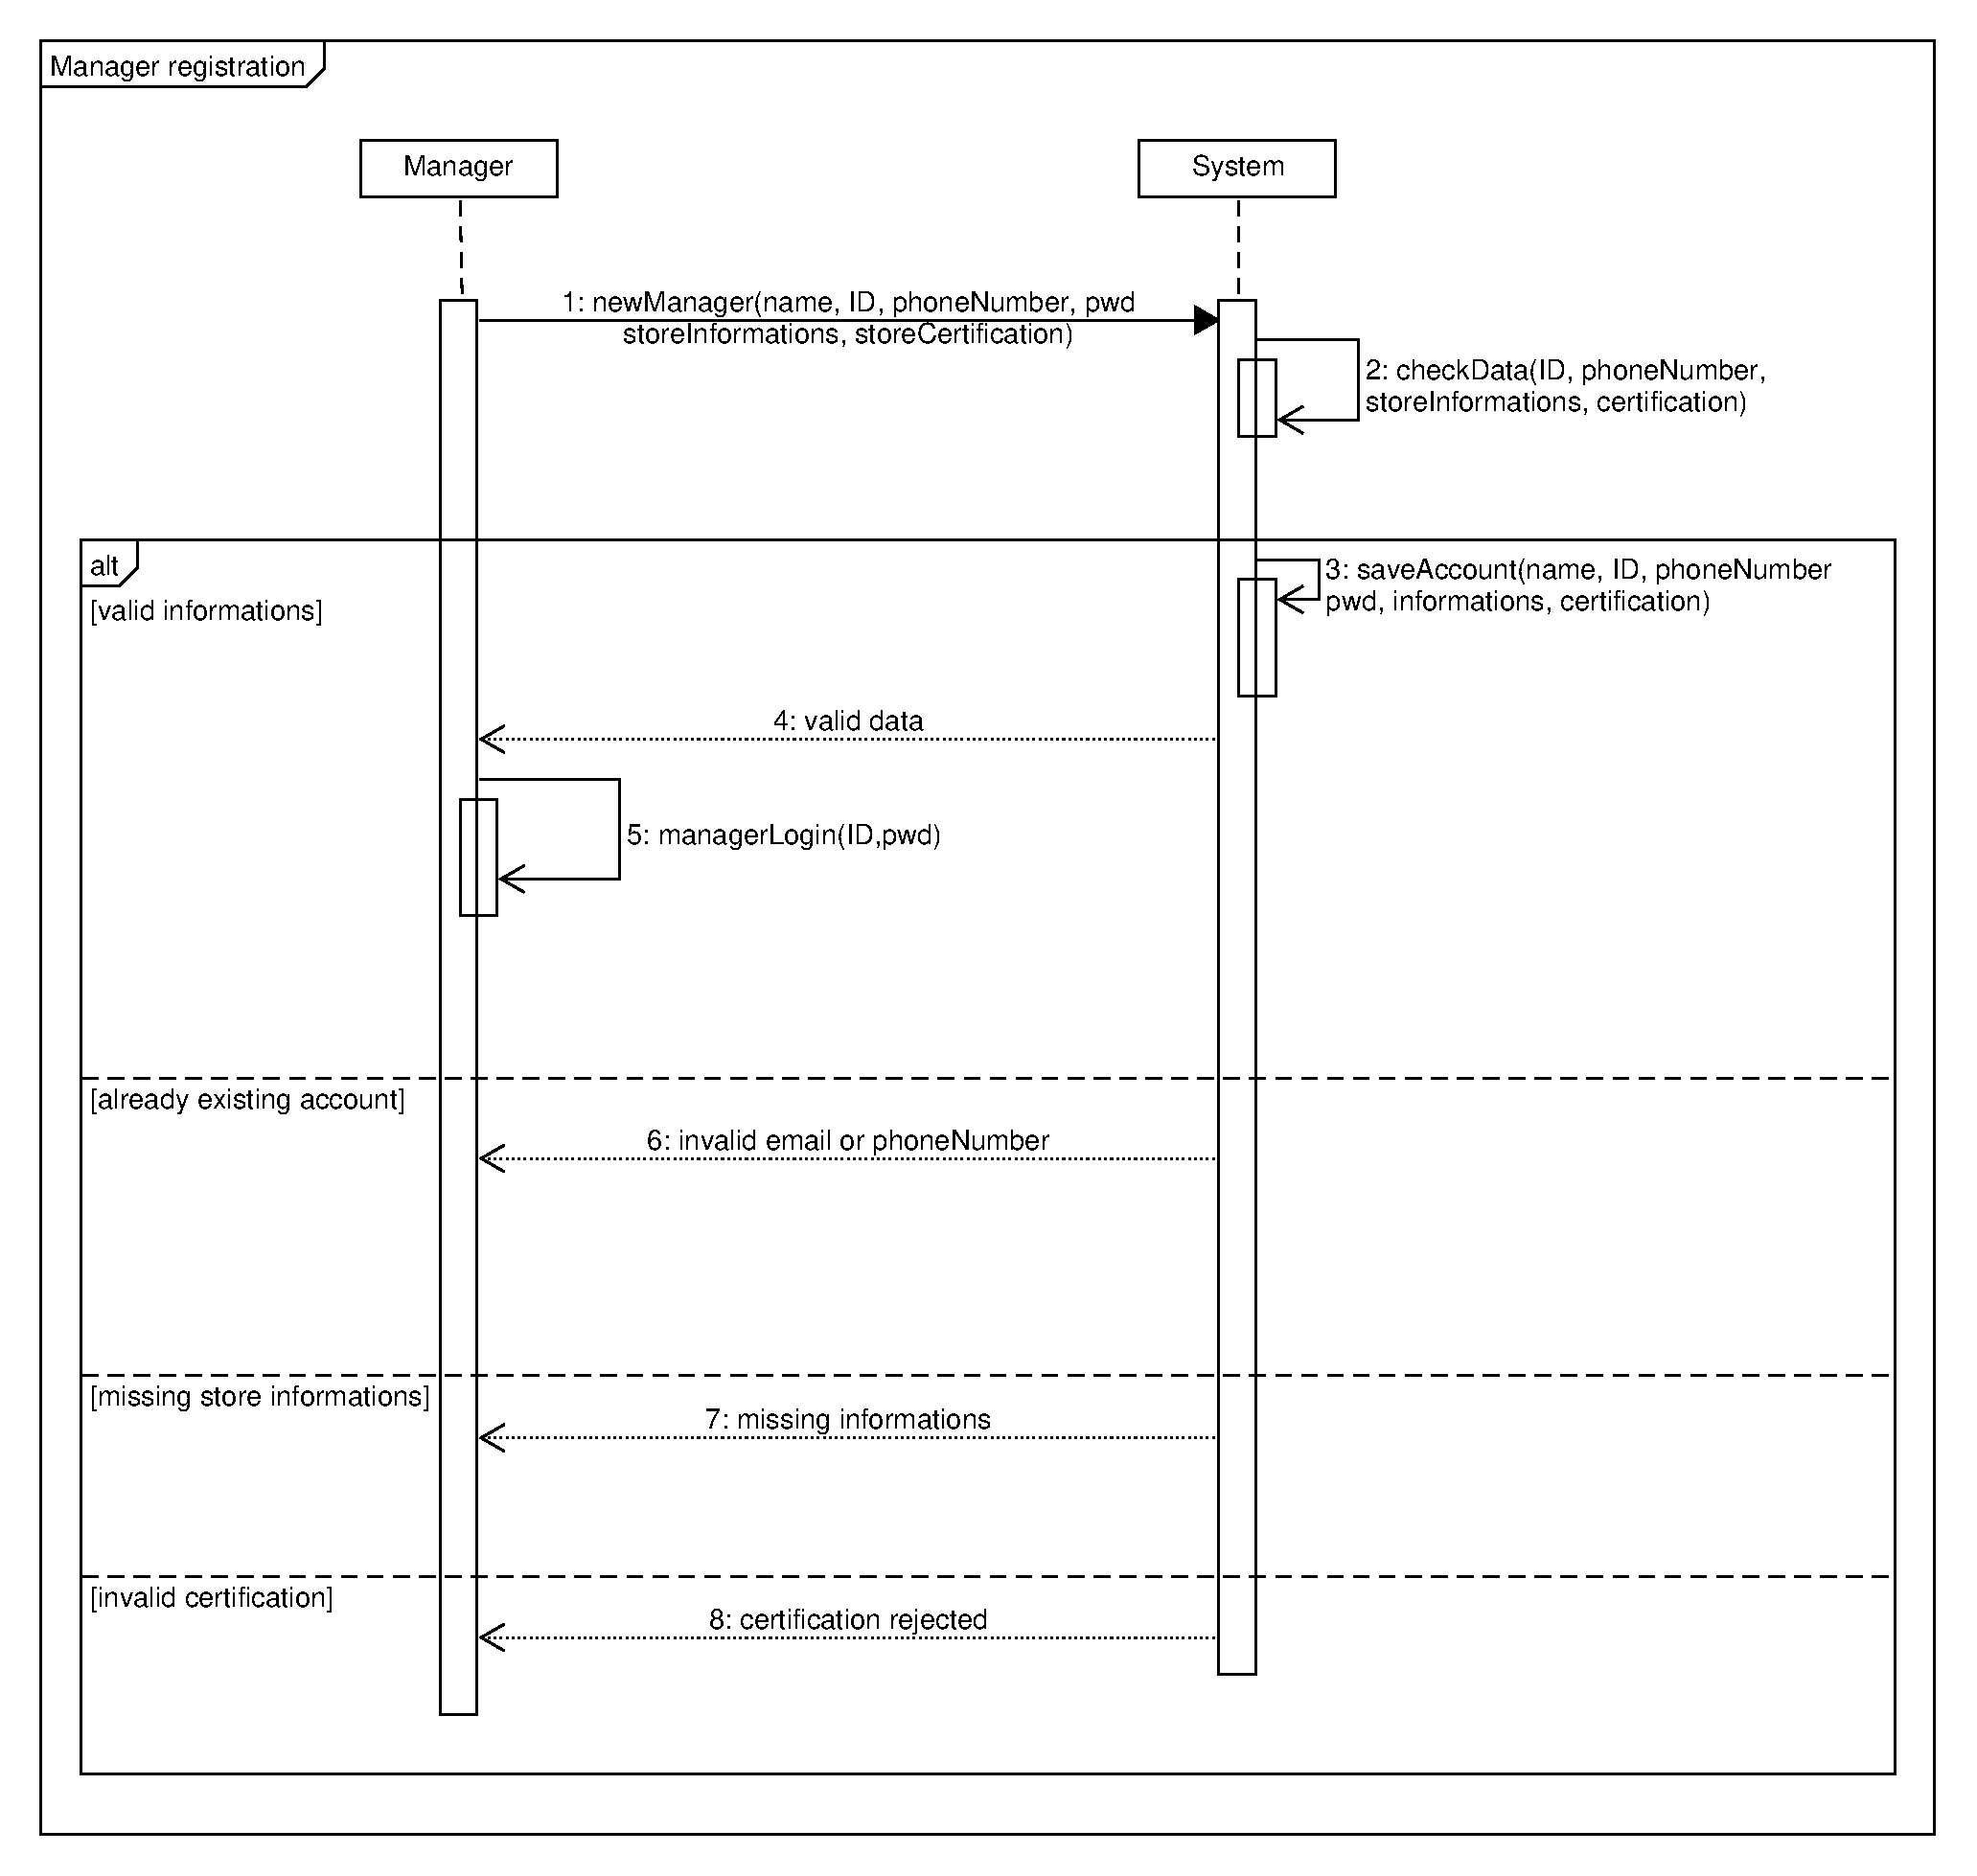
\includegraphics[scale=0.5]{SD/2_storeManagerRegistration.pdf}\\
									\caption{Sequence Diagram of Store Manager Registration}
								\end{adjustwidth}
							\end{figure}

						
						
					

				\end{center}

			\newpage


			\paragraph{Login of a customer}
			
				\begin{center}
					
					\rowcolors{2}{}{gray!20}
					\rowcolors{1}{gray!20}{white}
					
					\begin{adjustwidth}{-2.8cm}{}
					\begin{tabular}[h!]{|m{7.5em}|m{36em}|}
						
						\hline
						\xrowht{5pt}
						Name & Login of a customer\\
						\xrowht{5pt}
						Actors & Customer\\
						\xrowht{5pt}
						Entry Condition & Customer is already registered to the application service\\
						\xrowht{5pt}
						Event Flow & \begin{enumerate}
							
							\itemsep-0.25em
							\item Customer accesses the application through its device
							\item Customer clicks on “Login as customer” button
							\item The system opens the “Login as customer” page
							\item Customer compiles the fields “Username” and “Password”
							\item Customer clicks on “Login” button
							\item The system opens the “Customer menu” page
							
						\end{enumerate}\\
						\xrowht{5pt}
						Exit Conditions & Customer has successfully logged in\\
						\xrowht{5pt}
						Exception & \begin{enumerate}
							
							\itemsep0em
							\item Customer enters invalid email
							\item Customer enters invalid password
							
						\end{enumerate}
						If one or more of the above situations occur, the application will throw an error message and will return to the “Login as customer” page\\		
						\hline
						
					\end{tabular}
					\end{adjustwidth}
					
					\begin{figure}[!h]
						\begin{adjustwidth} {-1.3cm}{}
							\centering
							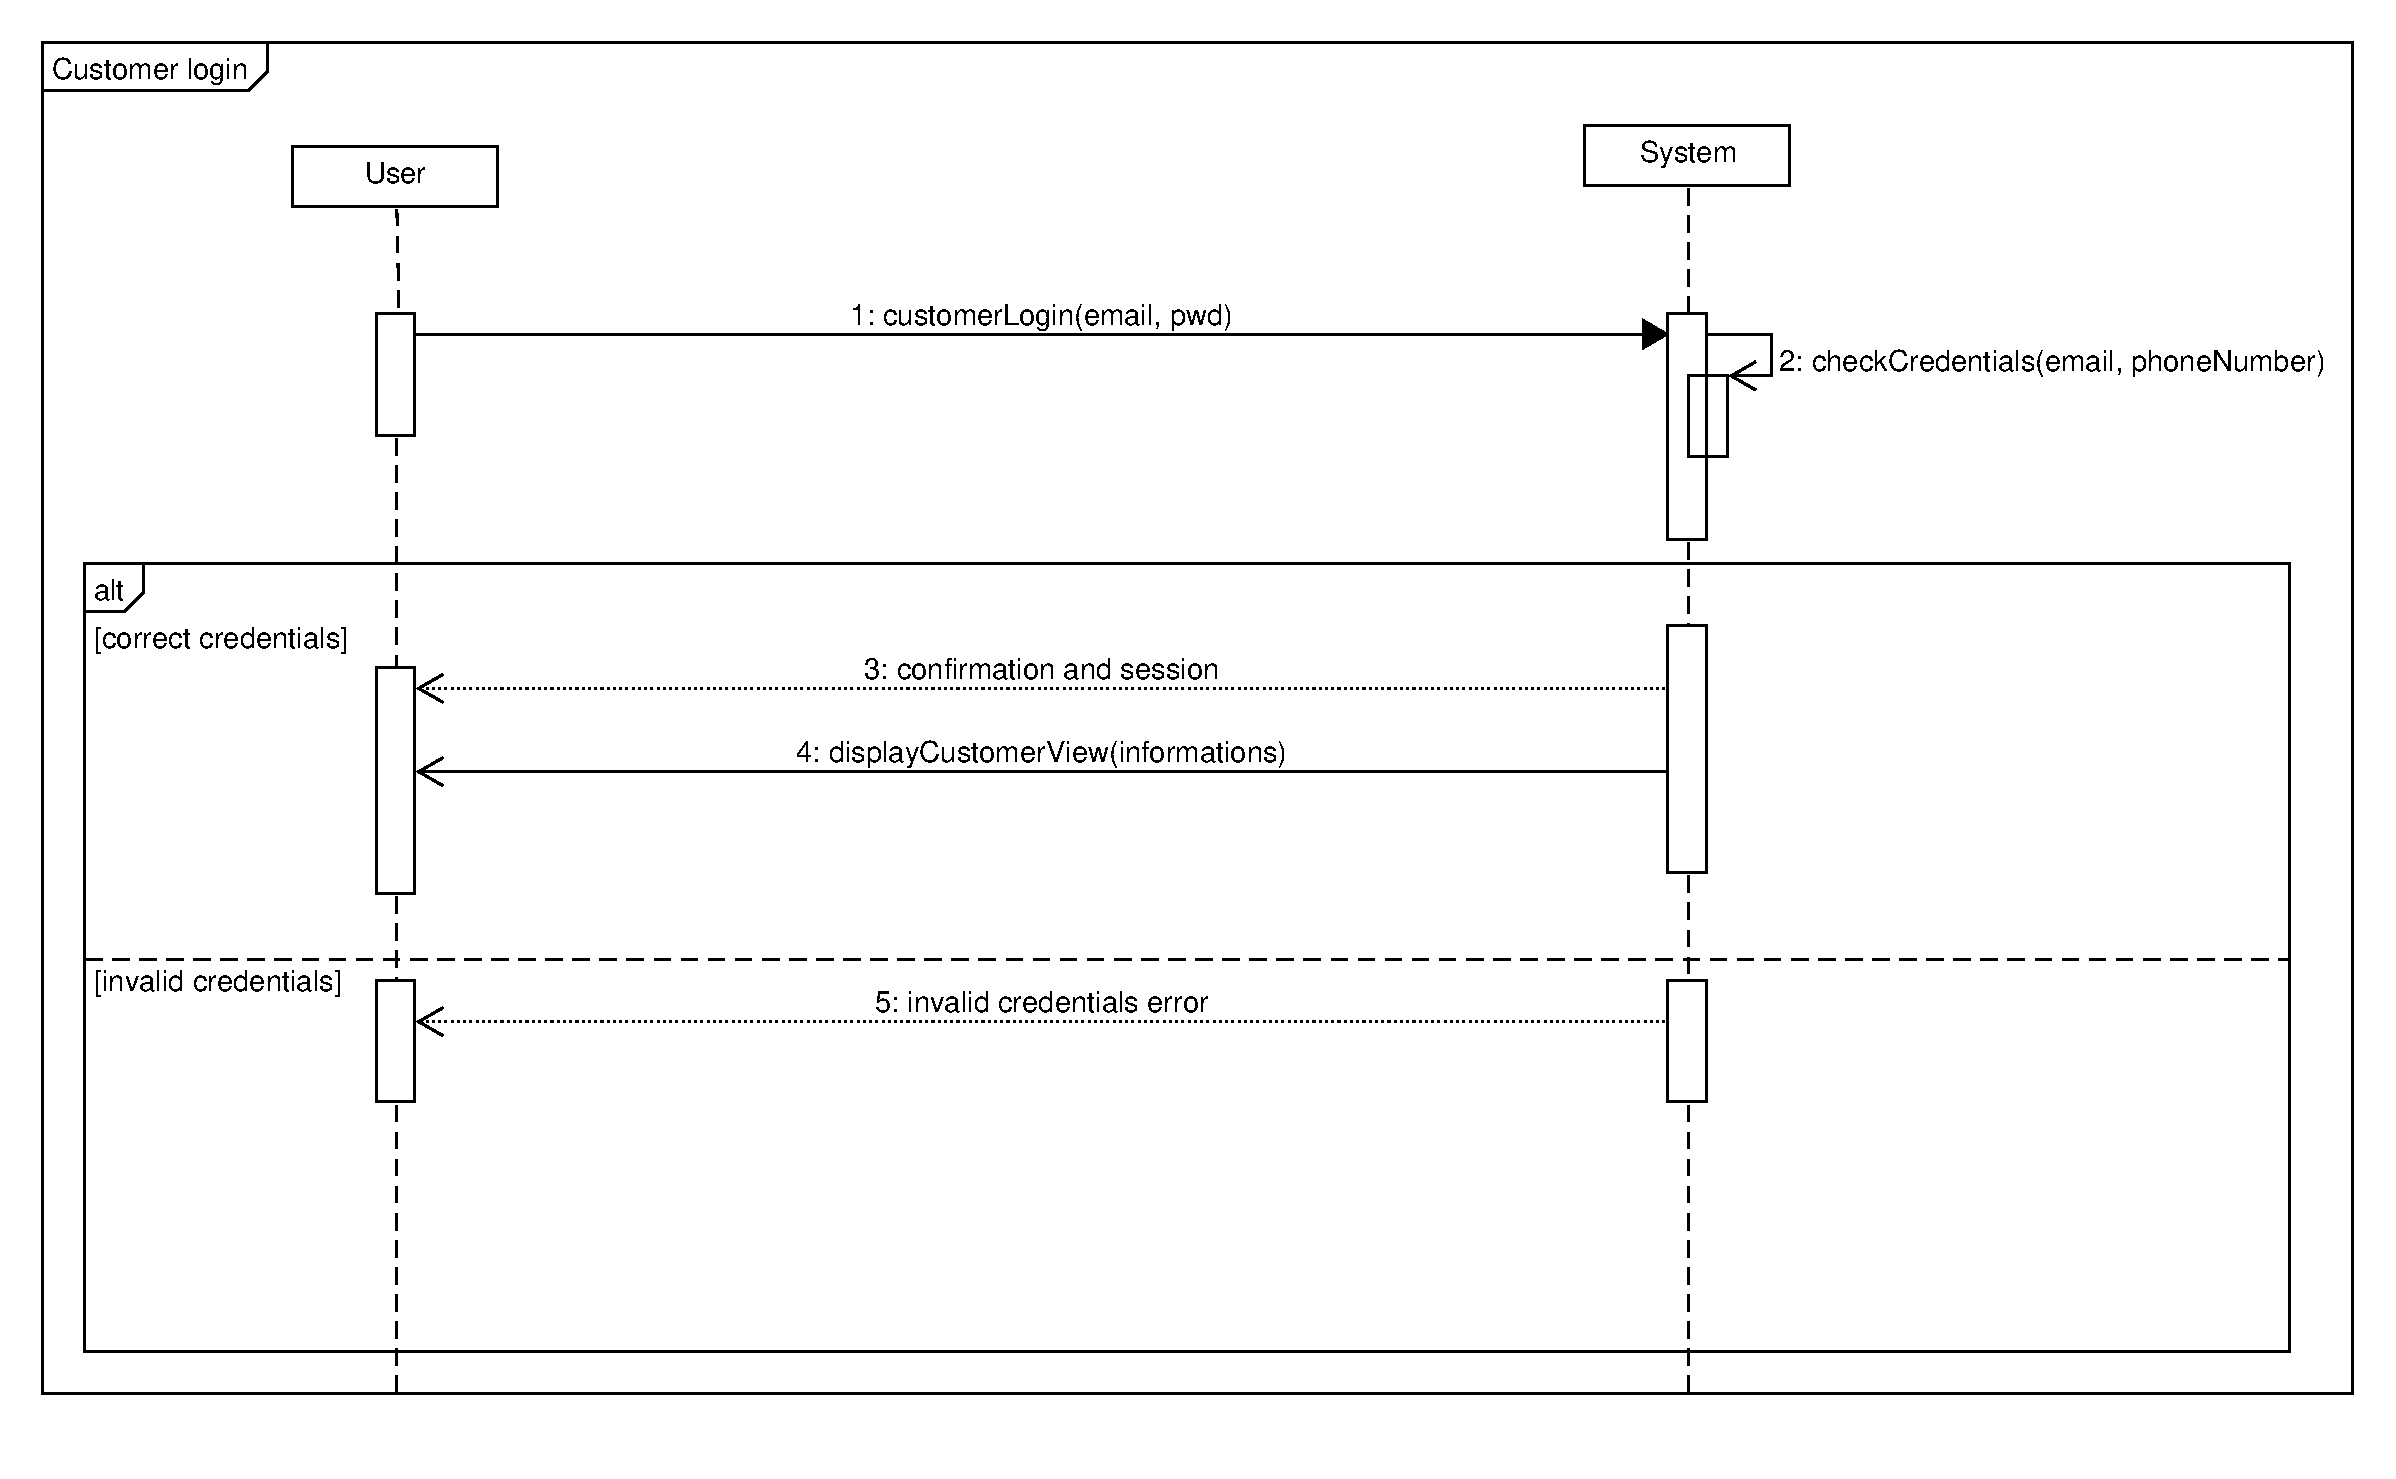
\includegraphics[scale=0.36]{SD/3_customerLogin.pdf}\\
							\caption{Sequence Diagram of Customer Login}
						\end{adjustwidth}
					\end{figure}

					\begin{itemize}
					\bigskip
					\bigskip
					\bigskip
					 {\bfseries Required functional requirements: }
					\item {\bfseries R3: } The system must allow customers to log in

					\end{itemize}

				\end{center}
			
					\bigskip
					\bigskip
					\bigskip
			\paragraph{Login of a store manager}
			
				\begin{center}
					
					\rowcolors{2}{}{gray!20}
					\rowcolors{1}{gray!20}{white}
					
					\begin{adjustwidth}{-2.8cm}{}
					\begin{tabular}[h!]{|m{7.5em}|m{36em}|}
						
						\hline
						\xrowht{5pt}
						Name & Login of a store manager\\
						\xrowht{5pt}
						Actors & Store manager\\
						\xrowht{5pt}
						Entry Condition & Store manager’s store is already registered to the application service\\
						\xrowht{5pt}
						Event Flow & \begin{enumerate}
							
							\itemsep-0.25em
							\item Store manager accesses the application through its device
							\item Store manager clicks on “Login as store” button
							\item The system opens the “Login as store” page
							\item Store manager compiles the fields “ID” and “Password”
							\item Store manager clicks on “Login” button
							\item The system opens the “Store menu” page
							
						\end{enumerate}\\
						\xrowht{5pt}
						Exit Conditions & Store manager has successfully logged in\\
						\xrowht{5pt}
						Exception & \begin{enumerate}
							
							\itemsep-0.25em
							\item Store manager enters invalid ID
							\item Store manager enters invalid Password
							
						\end{enumerate}
						If one or more of the above situations occur, the application will throw an error message and will return to the “Login as store” page\\		
						\hline
						
					\end{tabular}
					\end{adjustwidth}

\begin{itemize}
					\bigskip
					\bigskip
					\bigskip
					 {\bfseries Required functional requirements: }
					\item {\bfseries R4: } The system must allow store managers to log in
					

					\end{itemize}

							\begin{figure}
								\begin{adjustwidth} {-3cm}{}
									\centering
									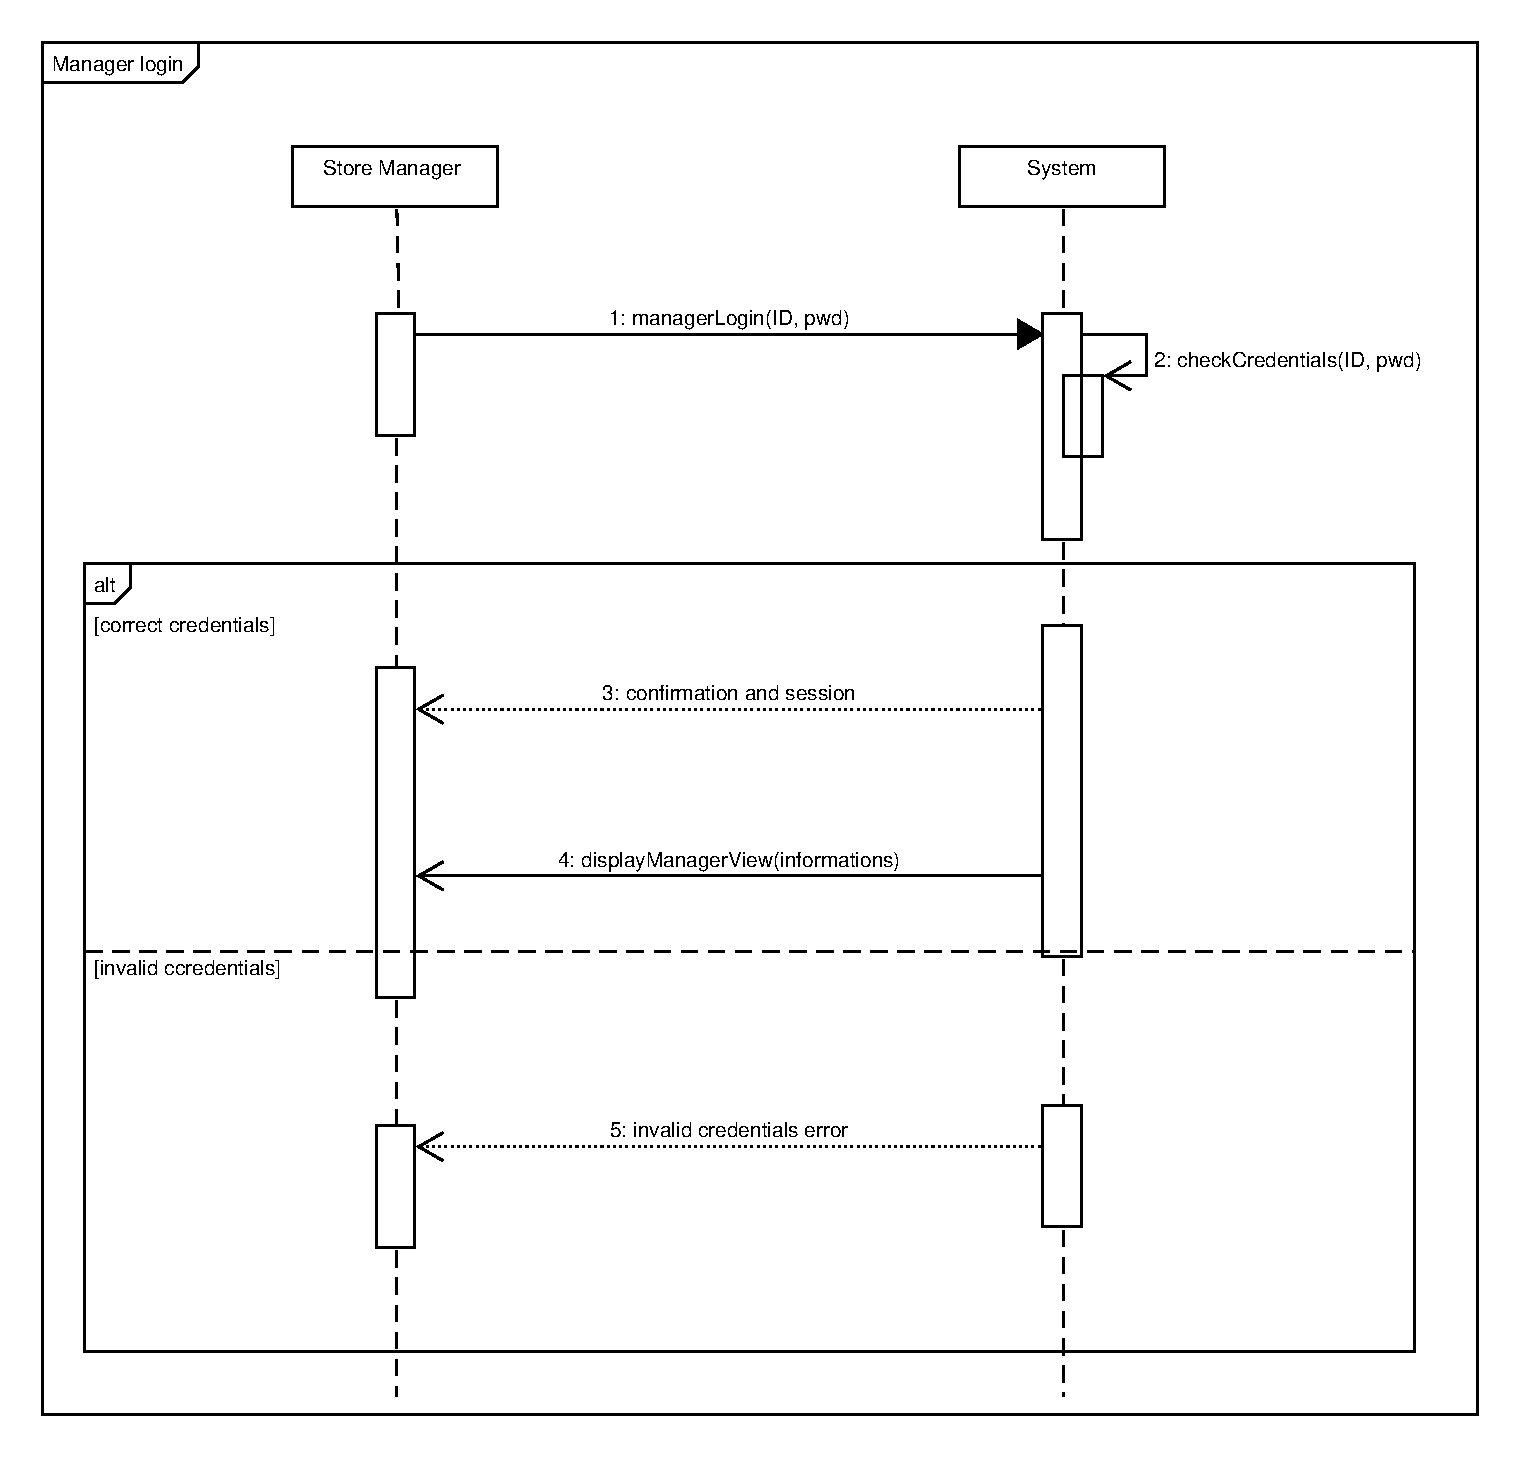
\includegraphics[scale=0.7]{SD/4_managerLogin.pdf}\\
									\caption{Sequence Diagram of Store Manager Login}
								\end{adjustwidth}
							\end{figure}
					
				\end{center}
				\newpage
			
			\paragraph{Customer makes a reservation}
			
				\begin{center}
					
					\rowcolors{2}{}{gray!20}
					\rowcolors{1}{gray!20}{white}
					
					\begin{adjustwidth}{-2.8cm}{}
					\begin{tabular}[h!]{|m{7.5em}|m{36em}|}
						
						\hline
						\xrowht{5pt}
						Name & Customer makes a reservation\\
						\xrowht{5pt}
						Actors & Customer\\
						\xrowht{5pt}
						Entry Condition & Customer is already logged in the application service\\
						\xrowht{5pt}
						Event Flow & \begin{enumerate}
							
							\itemsep-0.25em
							\item Customer clicks on “Make a reservation”
							\item The customer can see the list of stores in his city and can filter this list by choosing a specific chain from a drop down menu, selects a store and clicks on Next
							\item Customer can see the list of all possible objects’ category and can select some of them (optional), and then clicks on Next
							\item Customer can estimate a duration for his shopping, or let the system to do it, and then clicks on Next
							\item Customer can see two button, “As soon as possible” and “Choose a time slot”
							 
							\begin{enumerate}
								
								\itemsep-0.25em
								\item if the clicks on “As soon as possible” button, the system will check if it's possible to assign a ticket with a reasonable waiting times in the day of the request, and by assuring it won't be over the store's closing time.
								

									
									
									 If a ticket with low waiting time is generable, the system will generate it calculating the time nedded to reach the store, saves it on both itself and user's app, showing it on the latter.
									 otherwise, the system suggests him stores less crowded, if any. If so, user can choose between the options proposed, including staying at the selected store. Else, if the ticket is generable, it will be generated even if with a high waiting time.
									

								
								\item if the customer clicks on “Choose a time slot”, the user can choose a time slot among those availables on the “Time slots” page to generate and save a ticket, calculating the time needed to reach the store.
								
							\end{enumerate}
							
						\end{enumerate}\\
						\xrowht{5pt}
						Exit Conditions & Customer has successfully made a reservation\\
						\xrowht{5pt}
						Exception & \begin{enumerate}
							
							\itemsep-0.25em
							\item Customer click on a timeslot no longer available or tries to book more than the set limit of reservations per week
							
							The application will throw an error message and will reload the “Time slots” page (updating it)
							
							\item Customer doesn’t select any product category
							
							The application will throw an error and ask to select at least some item.
							
							\item Customer tries to get a ticket while he already have a unused one

							The application shows an error message and invite to use the pending ticket
							\item In the selected store where get a spot on the queue there isn't availability in the day, and there isn't any available near store 

							If the above situation occurs, the application will throw an error and leave the client the possibility to book his visit.
							
							
						\end{enumerate}
							\\
							\hline
						
						
					\end{tabular}
					\end{adjustwidth}
					
							\begin{figure}
								\begin{adjustwidth} {0cm}{}
									\centering
									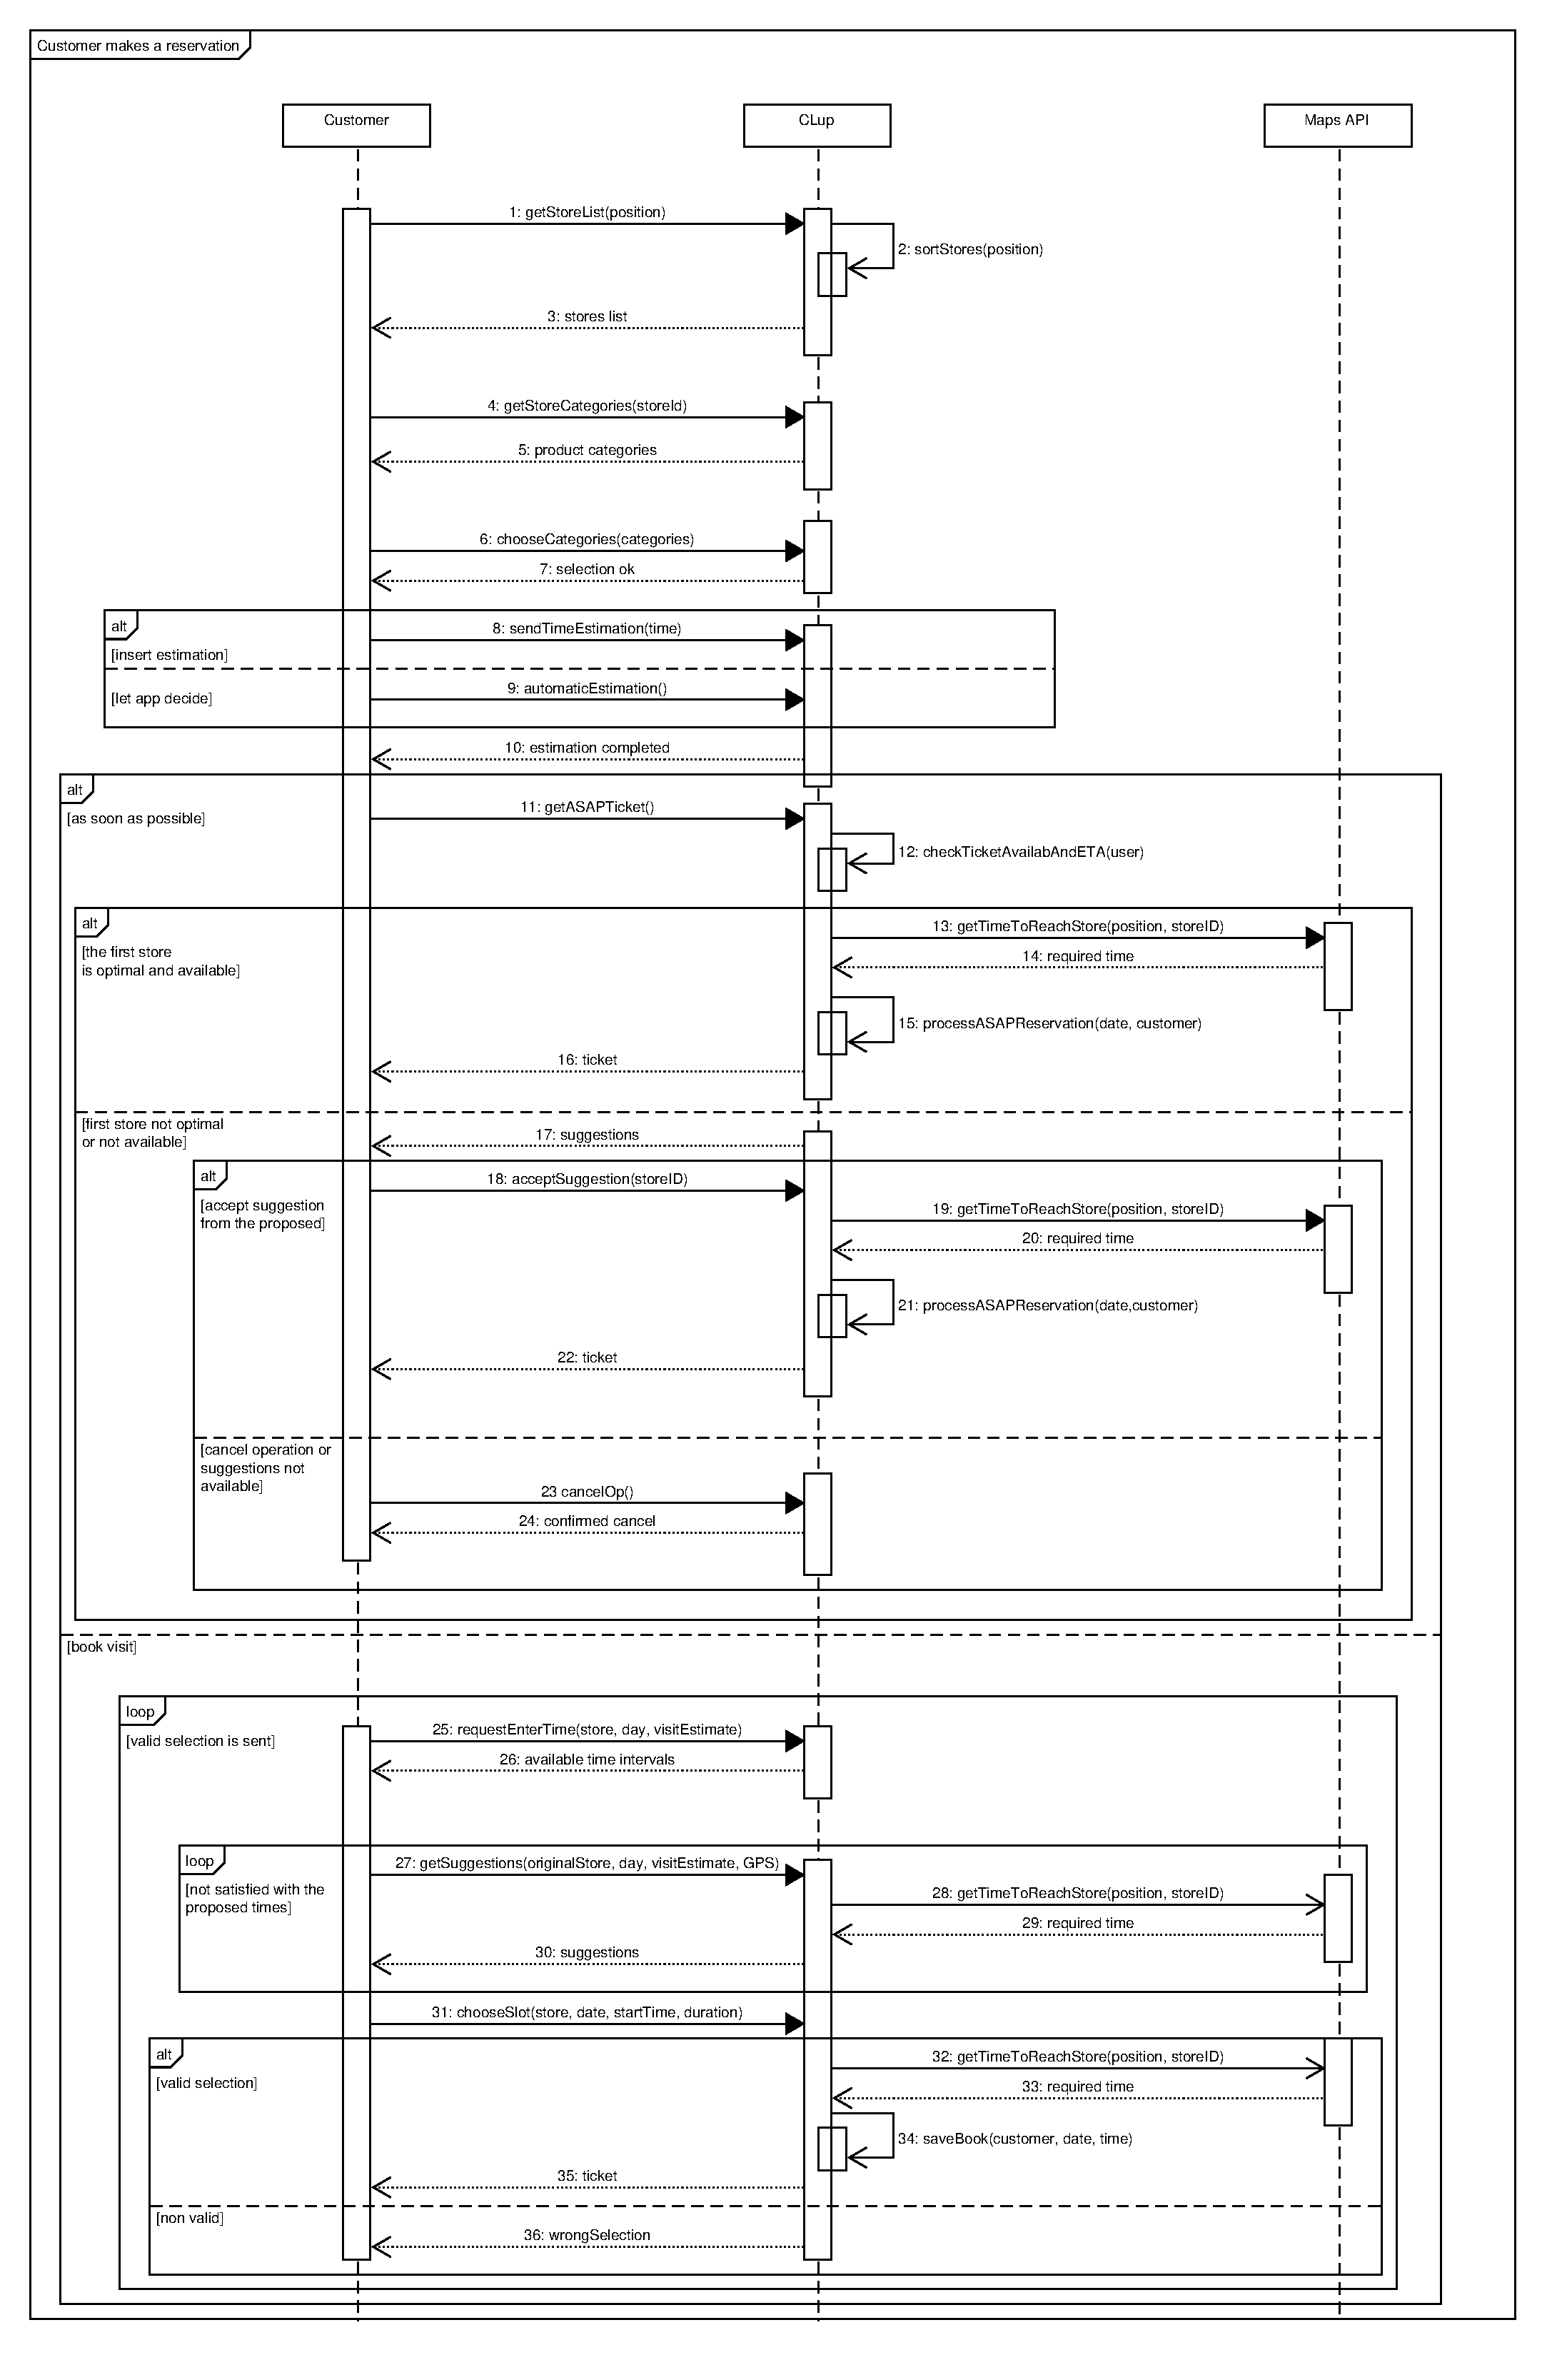
\includegraphics[scale=0.343]{SD/5_makeReservation.pdf}\\
									\caption{Sequence Diagram of Getting Ticket from App Procedure}
								\end{adjustwidth}
							\end{figure}

\begin{itemize}
					\bigskip
					\bigskip
					\bigskip
					 {\bfseries Required functional requirements: }


					\item {\bfseries R9: } The system allows the customers to select some or all the departments in
which the customers are interested in doing shopping
					\item {\bfseries R12: } The system must show the customers of the time periods in which they can
enter the store in order to respect the time selected by the customers


					\item {\bfseries R13: } The system have to make a reasonable estimate of when a user with a spot
on the queue is able to enter the store
					\item {\bfseries R15: } The system is able to ask for the position of the customers
					\item {\bfseries R23: } The system knows the situation in real time of each store

					\item {\bfseries R24: } The system takes trace of each customer entry and exit from the store
on the queue is able to enter the store
					\item {\bfseries R25: } The system contains a list of bookable stores
					\item {\bfseries R27: } The system can reasonably estimate the time needed from a specific user
to complete his shopping

					\item {\bfseries R28: } The system must save clients’ tickets
					\item {\bfseries R29: } The system should estimate when it must stop generating other tickets to
avoid turns after the closing time of the store

					\end{itemize}
				\end{center}
			
			\paragraph{Customer visualizes reservations}
			
				\begin{center}
					
					\rowcolors{2}{}{gray!20}
					\rowcolors{1}{gray!20}{white}
					
					\begin{adjustwidth}{-2.8cm}{}
					\begin{tabular}[h!]{|m{7.5em}|m{36em}|}
						
						\hline
						\xrowht{5pt}
						Name & Customer visualizes reservations\\
						\xrowht{5pt}
						Actors & Customer\\
						\xrowht{5pt}
						Entry Condition & Customer is already logged in the application service\\
						\xrowht{5pt}
						Event Flow & \begin{enumerate}
							
							\itemsep-0.25em
							\item Customer clicks on “Show requests” button
							\item The app show the list of bookings made and tickets requested
							\item The customer select the desired option
							\item The system opens the detail page of the selected option, that includes the “QR Code” and the number that should be called, among with the scheduled entry date and time and expected time when depart for the store. 
							
						\end{enumerate}\\
						\xrowht{5pt}
						Exit Conditions & Customer can visualize the reservation\\
						\xrowht{5pt}
						Exception & \begin{enumerate}
						\item The client has not pending requests
						If the above situation happen, the app shows an error message and bring the client to the home page.
						\end{enumerate}	
\\
						\hline
						
					\end{tabular}
					\end{adjustwidth}


\begin{itemize}
					\bigskip
					\bigskip
					\bigskip
					 {\bfseries Required functional requirements: }


					\item {\bfseries R5: }  The system allows the customers to view their visits
					\item {\bfseries R8: }  The system allows the customers to select their favorite means of transportation
					\item {\bfseries R15: } The system is able to ask for the position of the customers
					\item {\bfseries R28: } The system must save clients’ tickets






					\end{itemize}
				\end{center}
												\begin{figure}
								\begin{adjustwidth} {-2cm}{}
									\centering
									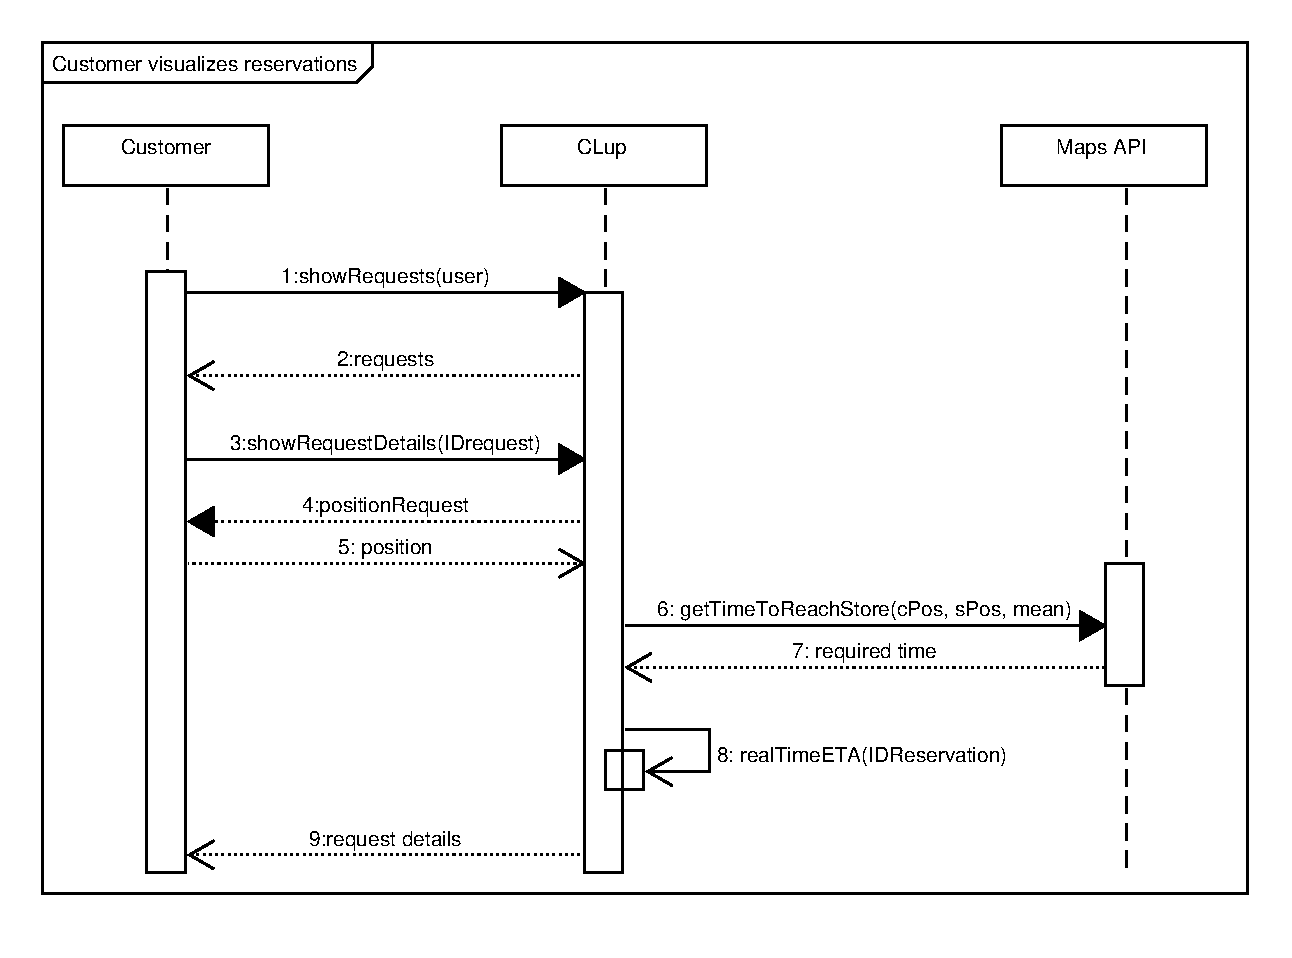
\includegraphics[scale=0.75]{SD/6_visualizeReservation.pdf}\\
									\caption{Sequence Diagram of Visualizing Customers' Reservations in app}
								\end{adjustwidth}
							\end{figure}
			\newpage
			\paragraph{Manager modifies store parameters}
			
				\begin{center}
					
					\rowcolors{2}{}{gray!20}
					\rowcolors{1}{gray!20}{white}
					
					\begin{adjustwidth}{-2.8cm}{}
					\begin{tabular}[h!]{|m{7.5em}|m{36em}|}
						
						\hline
						\xrowht{5pt}
						Name & Store manager modifies store parameters\\
						\xrowht{5pt}
						Actors & Store manager\\
						\xrowht{5pt}
						Entry Condition & Store manager is already logged in the application service\\
						\xrowht{5pt}
						Event Flow & \begin{enumerate}
							
							\itemsep-0.25em
							\item Store manager clicks on “Modify parameters” button
							\item Store manager can see both the parameters relatives to the whole store (eg. ID, Pwd, Opening and Closing Time), and each department with its parameters (max capacity and simultaneous allowed bookings)
							
							\begin{enumerate}
								
								\itemsep0em
								\item Store manager modify one, more or none of the parameters of the store or of some departements (clicking on the pencil shaped button of the desidered department)
								\item Store manager choose to add/delete some department respectively clicking on "Add a department" and on the bin shaped button of the desidered department
								\item Store manager clicks on Save Changes
					
								
							\end{enumerate}
							\item The system saves and processe the changes (notifying clients if necessary) and bring him back to “Store menu” page
							
						\end{enumerate}\\
						\xrowht{5pt}
						Exit Conditions & Store manager has successfully updated store parameters\\
						\xrowht{5pt}
						Exception & \begin{enumerate}
							
							\itemsep-0.25em
							\item Store managers enters an invalid value for one or more parameters
							\item The store manager tries to add an already existing department

							
						\end{enumerate}
					
						If the above situation occur, the application will throw an error message and will return to “Modify parameters” page\\	
						\hline
						
					\end{tabular}
					\end{adjustwidth}

					\bigskip

					\begin{itemize}
					\medskip
					 {\bfseries Required functional requirements: }


					\item {\bfseries R16: } The system permits to store manager to modify the maximum capacity of the store’s departments

					\item {\bfseries R28: } The system allows the manager to establish the maximum simultaneously allowed booked clients in a specific department
					\item {\bfseries R14: }  The system can send notification to the clients
					\item {\bfseries R22: } The store manager can handle the opening and closing time of the store
					\end{itemize}					

							\begin{figure}[!h]
								\begin{adjustwidth} {-1,1cm}{}
									\centering
									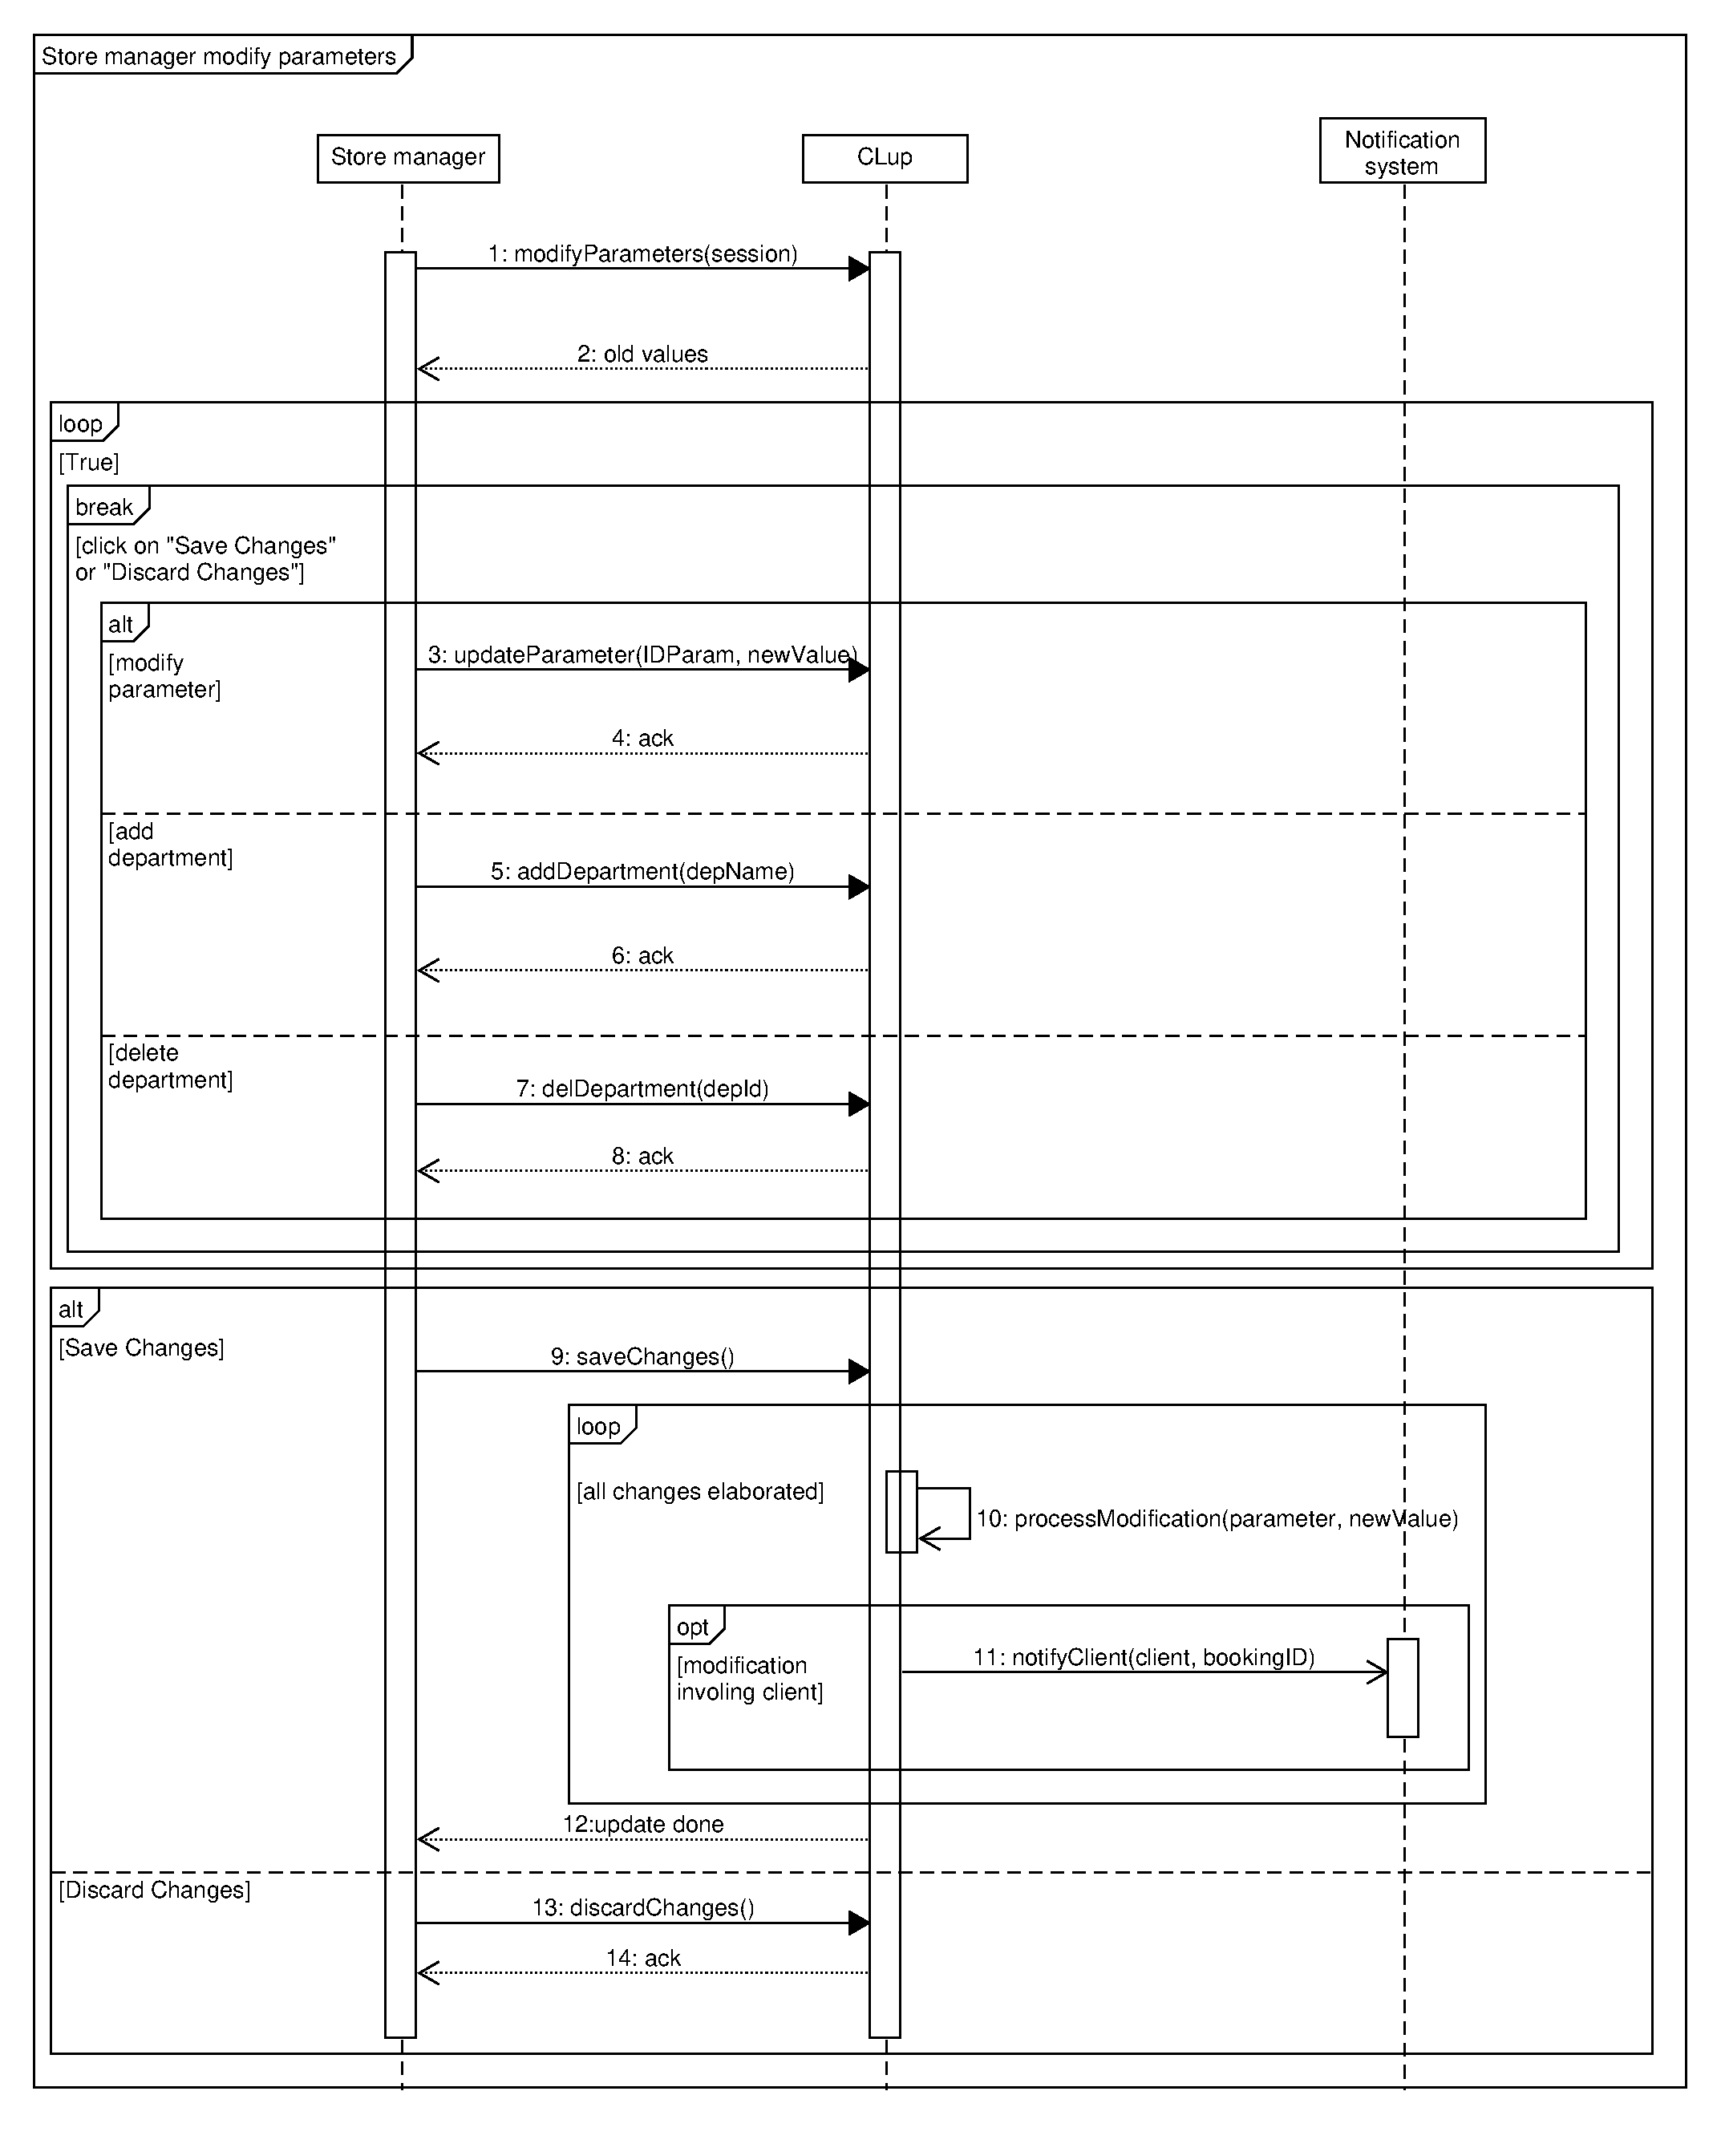
\includegraphics[scale=0.385]{SD/7_modifyParameters.pdf}\\
									\caption{Sequence Diagram of Visualizing Customers' Reservations in app}
								\end{adjustwidth}
							\end{figure}

				\end{center}



\newpage
			
			\paragraph{The store manager monitors the store situation}
			
				\begin{center}
					
					\rowcolors{2}{}{gray!20}
					\rowcolors{1}{gray!20}{white}
					
					\begin{adjustwidth}{-2.8cm}{}
					\begin{tabular}[h!]{|m{7.5em}|m{36em}|}
						\hline
						\xrowht{5pt}
						Name & Store manager monitors store situation\\
						\xrowht{5pt}
						Actors & Store manager\\
						\xrowht{5pt}
						Entry Condition & Store manager has opened the app and is already logged in\\
						\xrowht{5pt}
						Event Flow & \begin{enumerate}
							
							\itemsep-0.25em
							\item Manager clicks on “Monitor store” button
							\item The app shows a page with statistics on the store, including number of people inside the store, percentage of store occupation and the number of daily access to the building
							
							\begin{enumerate}
								\item If the manager wants, he can see the same statistics per store zone by clicking the “monitor zones” button. The system will show all the zones sorted by criticity
							\end{enumerate}
							
						\end{enumerate}\\
						\xrowht{5pt}
						Exit Conditions & Store manager can see statistics on the store\\
						\xrowht{5pt}
						Exception & None\\	
						\hline
						
					\end{tabular}
					\end{adjustwidth}
				
				\begin{itemize}
					\medskip
					{\bfseries Required functional requirements: }
					
					
					\item {\bfseries R9: }  The system allows the customers to select some or all the departments in
					which the customers are interested in doing shopping
					\item {\bfseries R17: } The system permits to store manager to view the statistics of the store and its departments
					\item {\bfseries R24: } The system takes trace of each customer entry and exit from the store
				
				\end{itemize}
			
					\begin{figure}[!h]
						\begin{adjustwidth} {0cm}{}
							\centering
							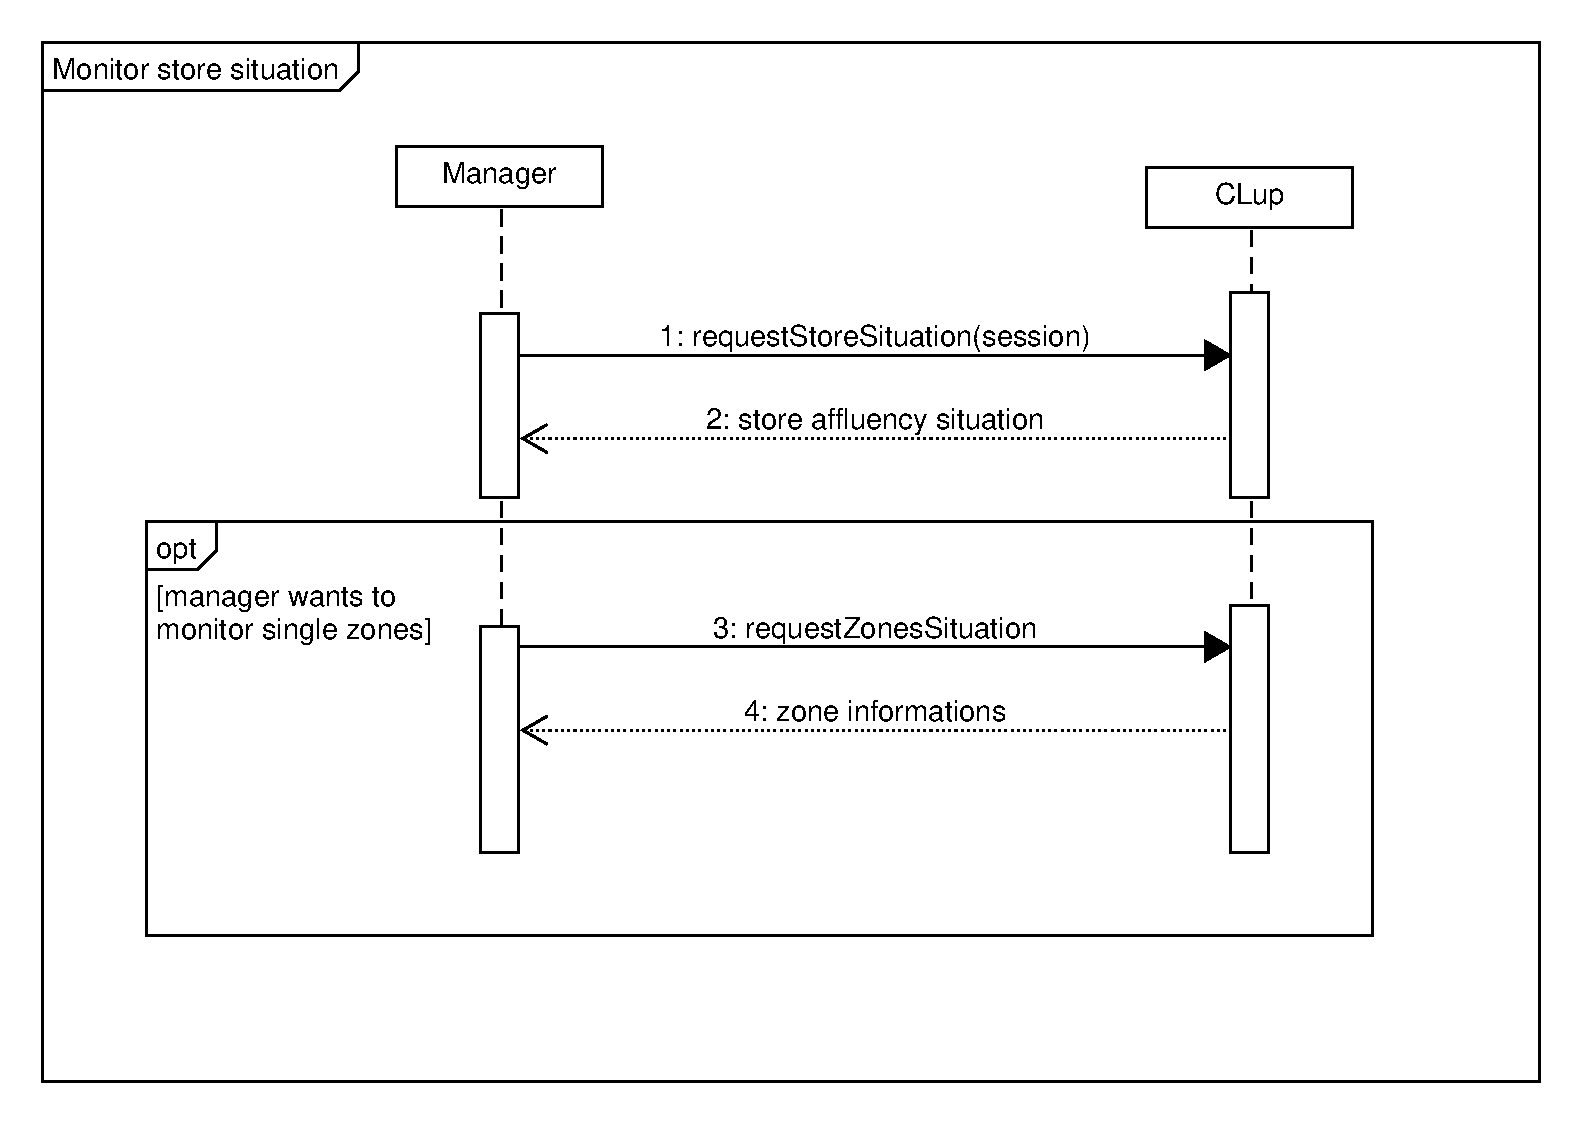
\includegraphics[scale=0.25]{SD/8_monitorStoreSituation.pdf}\\
							\caption{Sequence Diagram of Visualizing Store and Departments Situation}
						\end{adjustwidth}
					\end{figure}
					
				\end{center}
			
			\newpage
			\paragraph{The store manager manages customers bookings}
			
				\begin{center}
					
					\rowcolors{2}{}{gray!20}
					\rowcolors{1}{gray!20}{white}
					
					\begin{adjustwidth}{-2.8cm}{}
						\begin{tabular}[h!]{|m{7.5em}|m{36em}|}
							\hline
							\xrowht{5pt}
							Name & The store manager manages customers bookings\\
							\xrowht{5pt}
							Actors & Store manager\\
							\xrowht{5pt}
							Entry Condition & Store manager has opened the app and is already logged in\\
							\xrowht{5pt}
							Event Flow & \begin{enumerate}
								
								\itemsep-0.25em
								\item Manager clicks on “Manage bookings” button
								\item The app shows a list of reservations, with some of their details in preview (such as chosen date and time slot)
								\item The manager can choose one of them, and the app will show some possibilities to the manager
								
								\begin{enumerate}
									
									\item The manager can press on the button “Contact client” to contact the client for some reasons.
									
									\begin{enumerate}
										
										\item The manager can choose to contact the client via mail clicking on the button “Email option”
										
										
											
											\item The app will show an interface where the manager can insert the text
											\item The manger clicks on the “Send” button to send the message
											
										
									
									
									
										\item The app returns to the previous page
										
										
									\end{enumerate}
								
									\item The manager can click on the button “Cancel booking” to cancel a reservation
									
									\begin{enumerate}
										
										\item The app will show a dialog box where the manager can put-in an optional message, explaining the reasons of the cancel
										\item The manager clicks on the “Delete button”
										\item The app will show a confirmation box to ask if the manager is sure to proceed
										\item The manager clicks on “Yes” to confirm the deletion
										\item The app closes the dialog box
										
									\end{enumerate}
								
									\item The manager can choose to reschedule a booking
									
									\begin{enumerate}
										
										\item The app will show a dialog box where the manager can choose a new time slot and insert a message explaining the reasons
										\item The manager clicks on “Modify” to modify the booking
										\item The app closes the dialog box
										
									\end{enumerate}
									
								\end{enumerate}
								
							\end{enumerate}\\
							\xrowht{5pt}
							Exit Conditions & Store manager can manage the store and is able to edit reservations\\
							\xrowht{5pt}
							Exception & None\\	
							\hline
							
						\end{tabular}
					\end{adjustwidth}
				\newpage
					\begin{figure}[!h]
						\begin{adjustwidth} {-1,5cm}{}
							\centering
							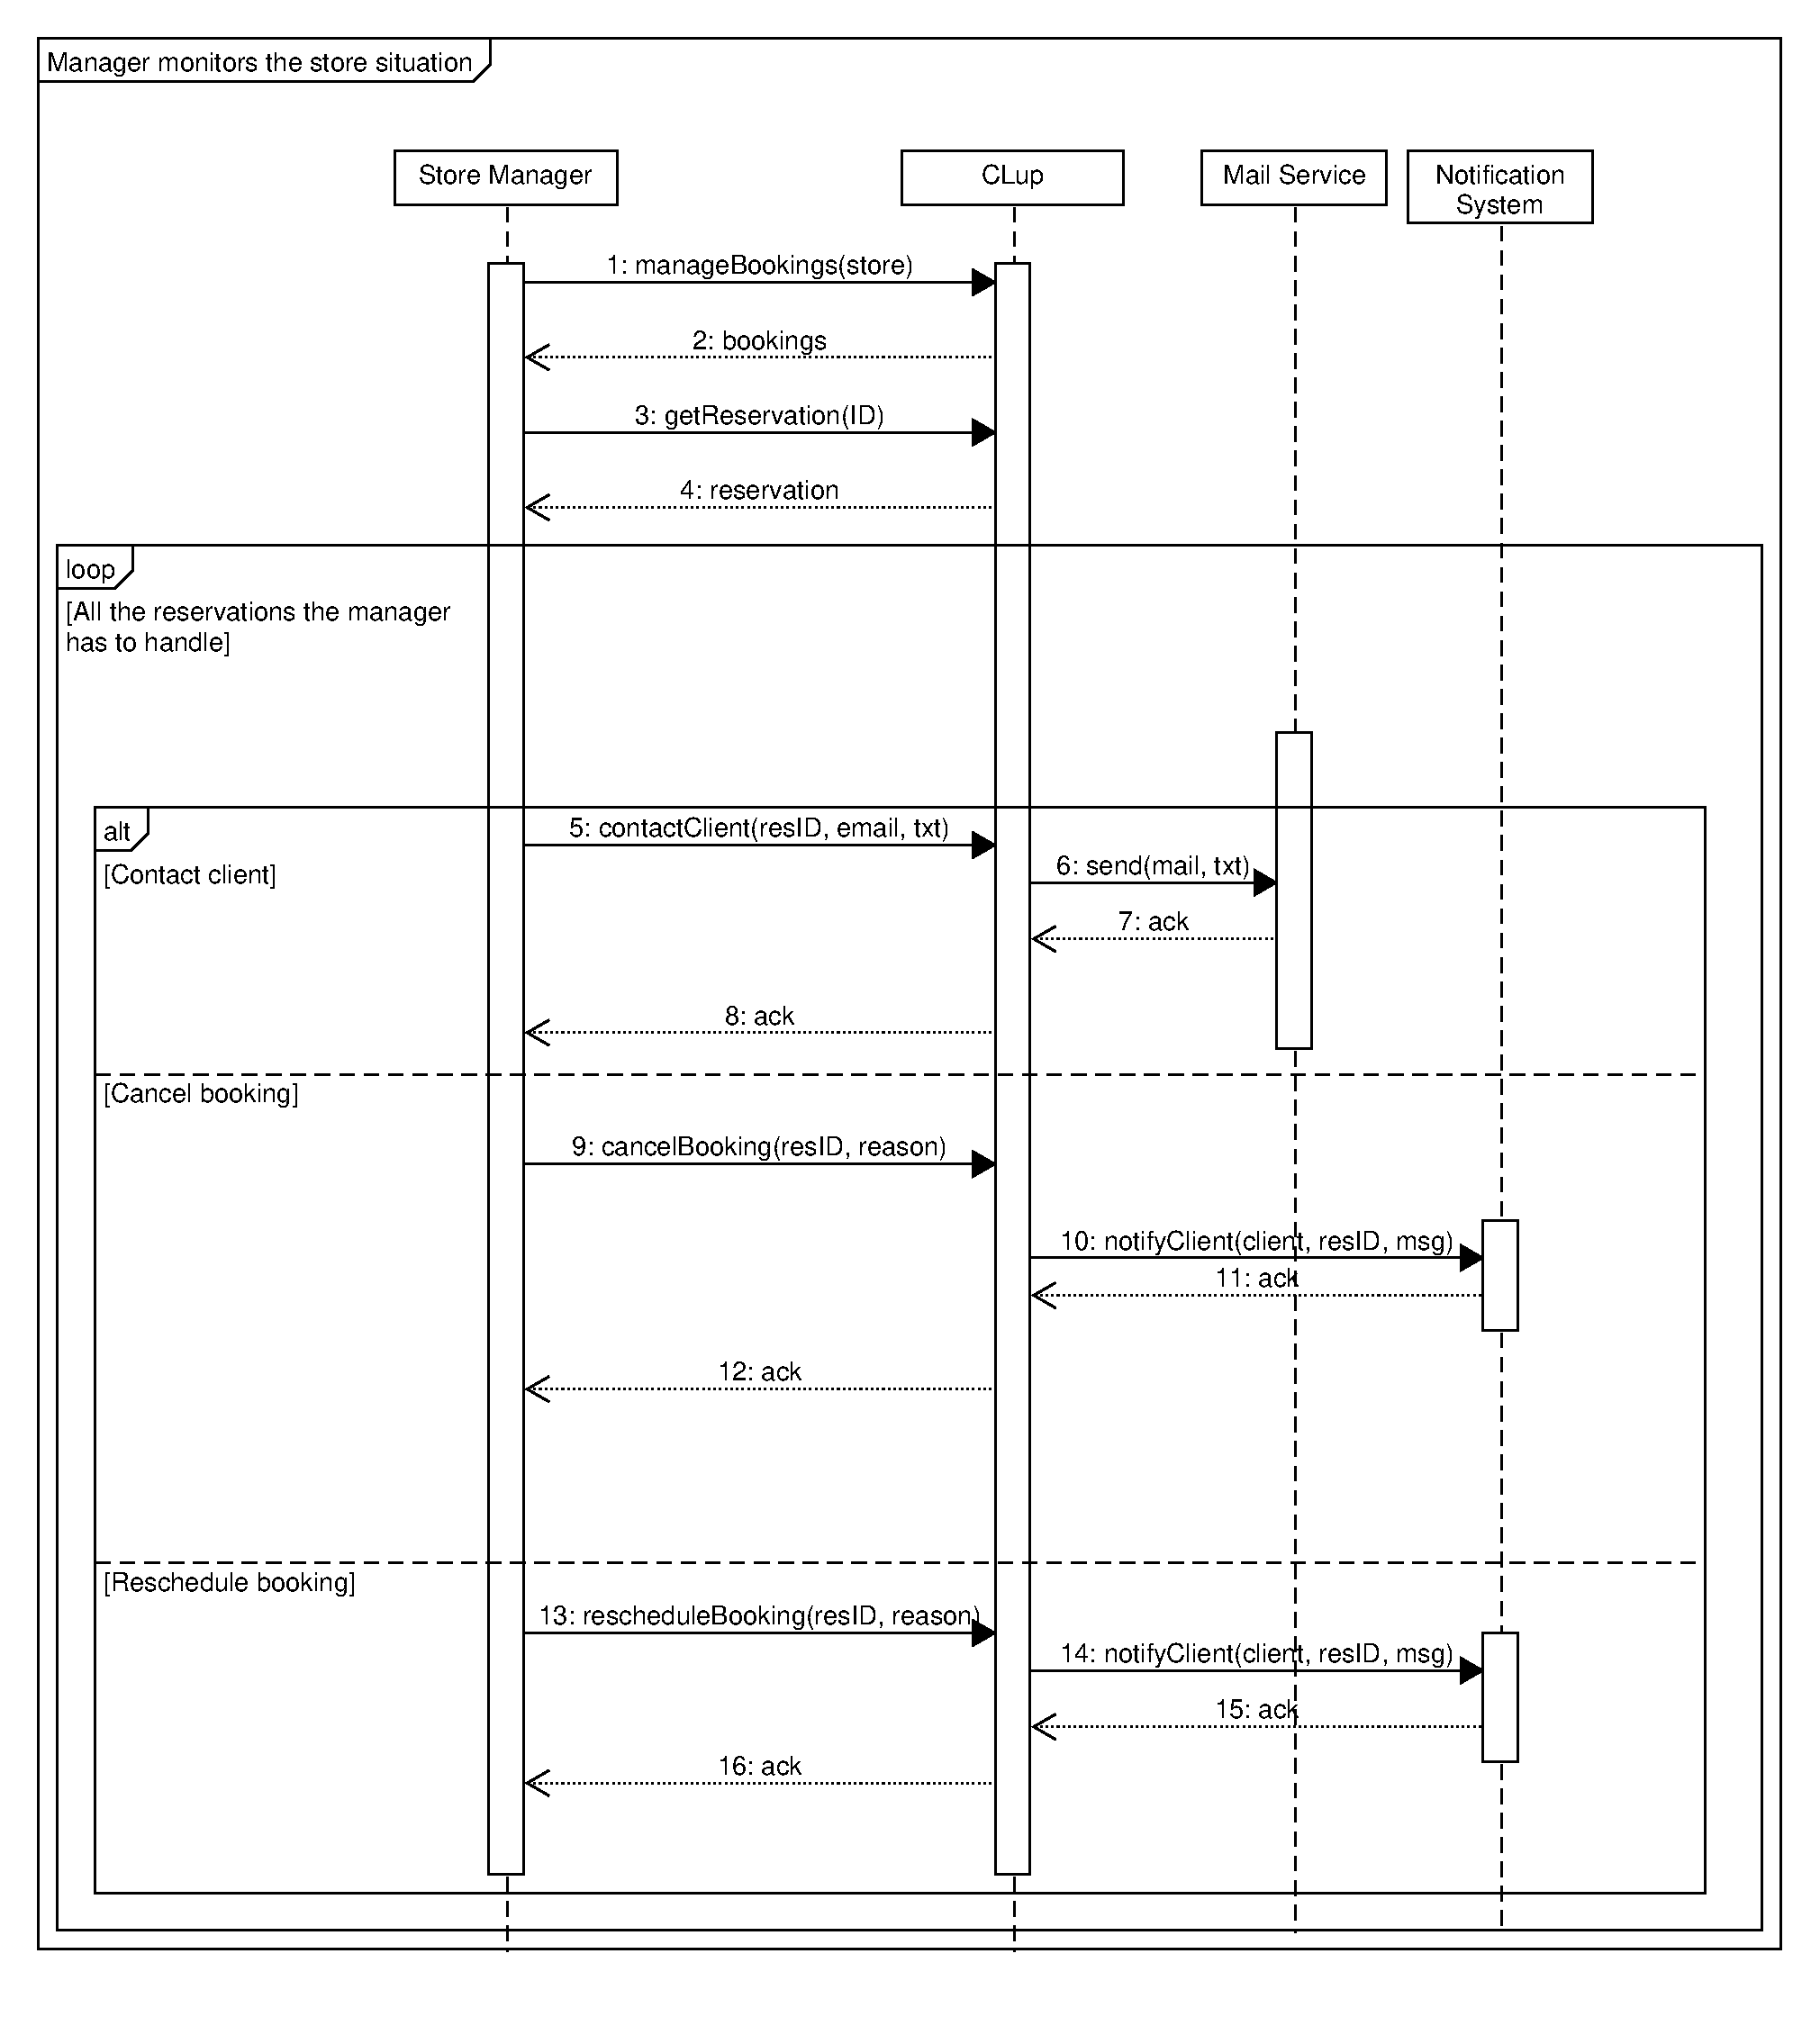
\includegraphics[scale=0.42]{SD/9_manageReservations(store)}\\
							\caption{Sequence Diagram of Visualizing Store and Departments Situation}
						\end{adjustwidth}
					\end{figure}
					\begin{itemize}
						\medskip
						
						{\bfseries Required functional requirements: }
						
						\item {\bfseries R14: } The system can send notification to the clients
						\item {\bfseries R19: }  The store manager can view the reservation of each client
						\item {\bfseries R20: } The store manager can modify the reservation of each client
						\item {\bfseries R21: } The store manager can cancel the reservation of each client
						\item {\bfseries R28: } The system must save clients’ tickets
						\item {\bfseries R32: } The system is able to send emails
						

					\end{itemize}	
					
				\end{center}
			
			\paragraph{Customers reservations management}
			
				\begin{center}
					
					\rowcolors{2}{}{gray!20}
					\rowcolors{1}{gray!20}{white}
					
					
					\begin{adjustwidth}{-2.8cm}{}
					\begin{tabular}[h!]{|m{7.5em}|m{36em}|}
							\hline
							\xrowht{5pt}
							Name & Customers reservations management\\
							\xrowht{5pt}
							Actors & Customer\\
							\xrowht{5pt}
							Entry Condition & The customer has the application opened, is logged in and has at least one pending request\\
							\xrowht{5pt}
							Event Flow & \begin{enumerate}
								
								\itemsep-0.25em
								\item The user press on the “Show requests” button
								\item The app shows a page with the requests made by the client
								\item The user selects the desidered requests
								\item The app will show the requests details
								\item The user press the “edit” button
								
								\begin{enumerate}
									
									\item If the selected requests is a ticket, the customer can delete it pressing the “Delete button”
									
									\begin{enumerate}
										
										\item The system will show a confirmation dialogue
										\item The client press the yes button
										\item The ticket is deleted and the app will return to the previous screen if there are other requests, or to the main menu otherwise
										
									\end{enumerate}
								
									\item If the selected request is a booking, the client can both click the delete button, and follow the above procedure or can select the “modify button”
									
									\begin{enumerate}
										
										\item If the modify button is selected, the app will restart the “Make a reservation process” described in Use Case n. 5. The customer can modify all the parameters of his reservation, including transforming it in a “As soon as possible ticket
										 
									\end{enumerate}
									
								\end{enumerate}
								
							\end{enumerate}\\
							\xrowht{5pt}
							Exit Conditions & The client can modify his reservation\\
							\xrowht{5pt}
							Exception & None\\	
							\hline
							
						\end{tabular}
					\end{adjustwidth}
					\begin{itemize}
						\medskip
						\newpage
						{\bfseries Required functional requirements: }
						
						
						\item {\bfseries R5: } The system allows the customers to view their visits
						\item {\bfseries R6: } The system allows the customers to cancel their visits
						\item {\bfseries R7: } The system allows the customers to modify their visits
						
						\item {\bfseries R8: } The system allows the customers to select their favorite means of transportation
						\item {\bfseries R9: } The system allows the customers to select some or all the departments in
						which the customers are interested in doing shopping
						\item {\bfseries R11: } The system must consider the extimate shopping time insert by customers
						
						\item {\bfseries R12: } The system must show the customers of the time periods in which they can
						enter the store in order to respect the time selected by the customers
						\item {\bfseries R13: } The system have to make a reasonable estimate of when a user with a spot
						on the queue is able to enter the store
						\item {\bfseries R15: } The system is able to ask for the position of the customers
						\item {\bfseries R23: } The system knows the situation in real time of each store
						\item {\bfseries R27: } The system can reasonably estimate the time needed from a specific user
						to complete his shopping
						\item {\bfseries R28: } The system must save clients' tickets
						
						\item {\bfseries R29: } The system should estimate when it must stop generating other tickets to
						avoid turns after the closing time of the store
						to complete his shopping

						
						
					\end{itemize}
				

				\end{center}
			\newpage
			\begin{figure}[!htb]
				\begin{adjustwidth} {-3,3cm}{}
					\centering
					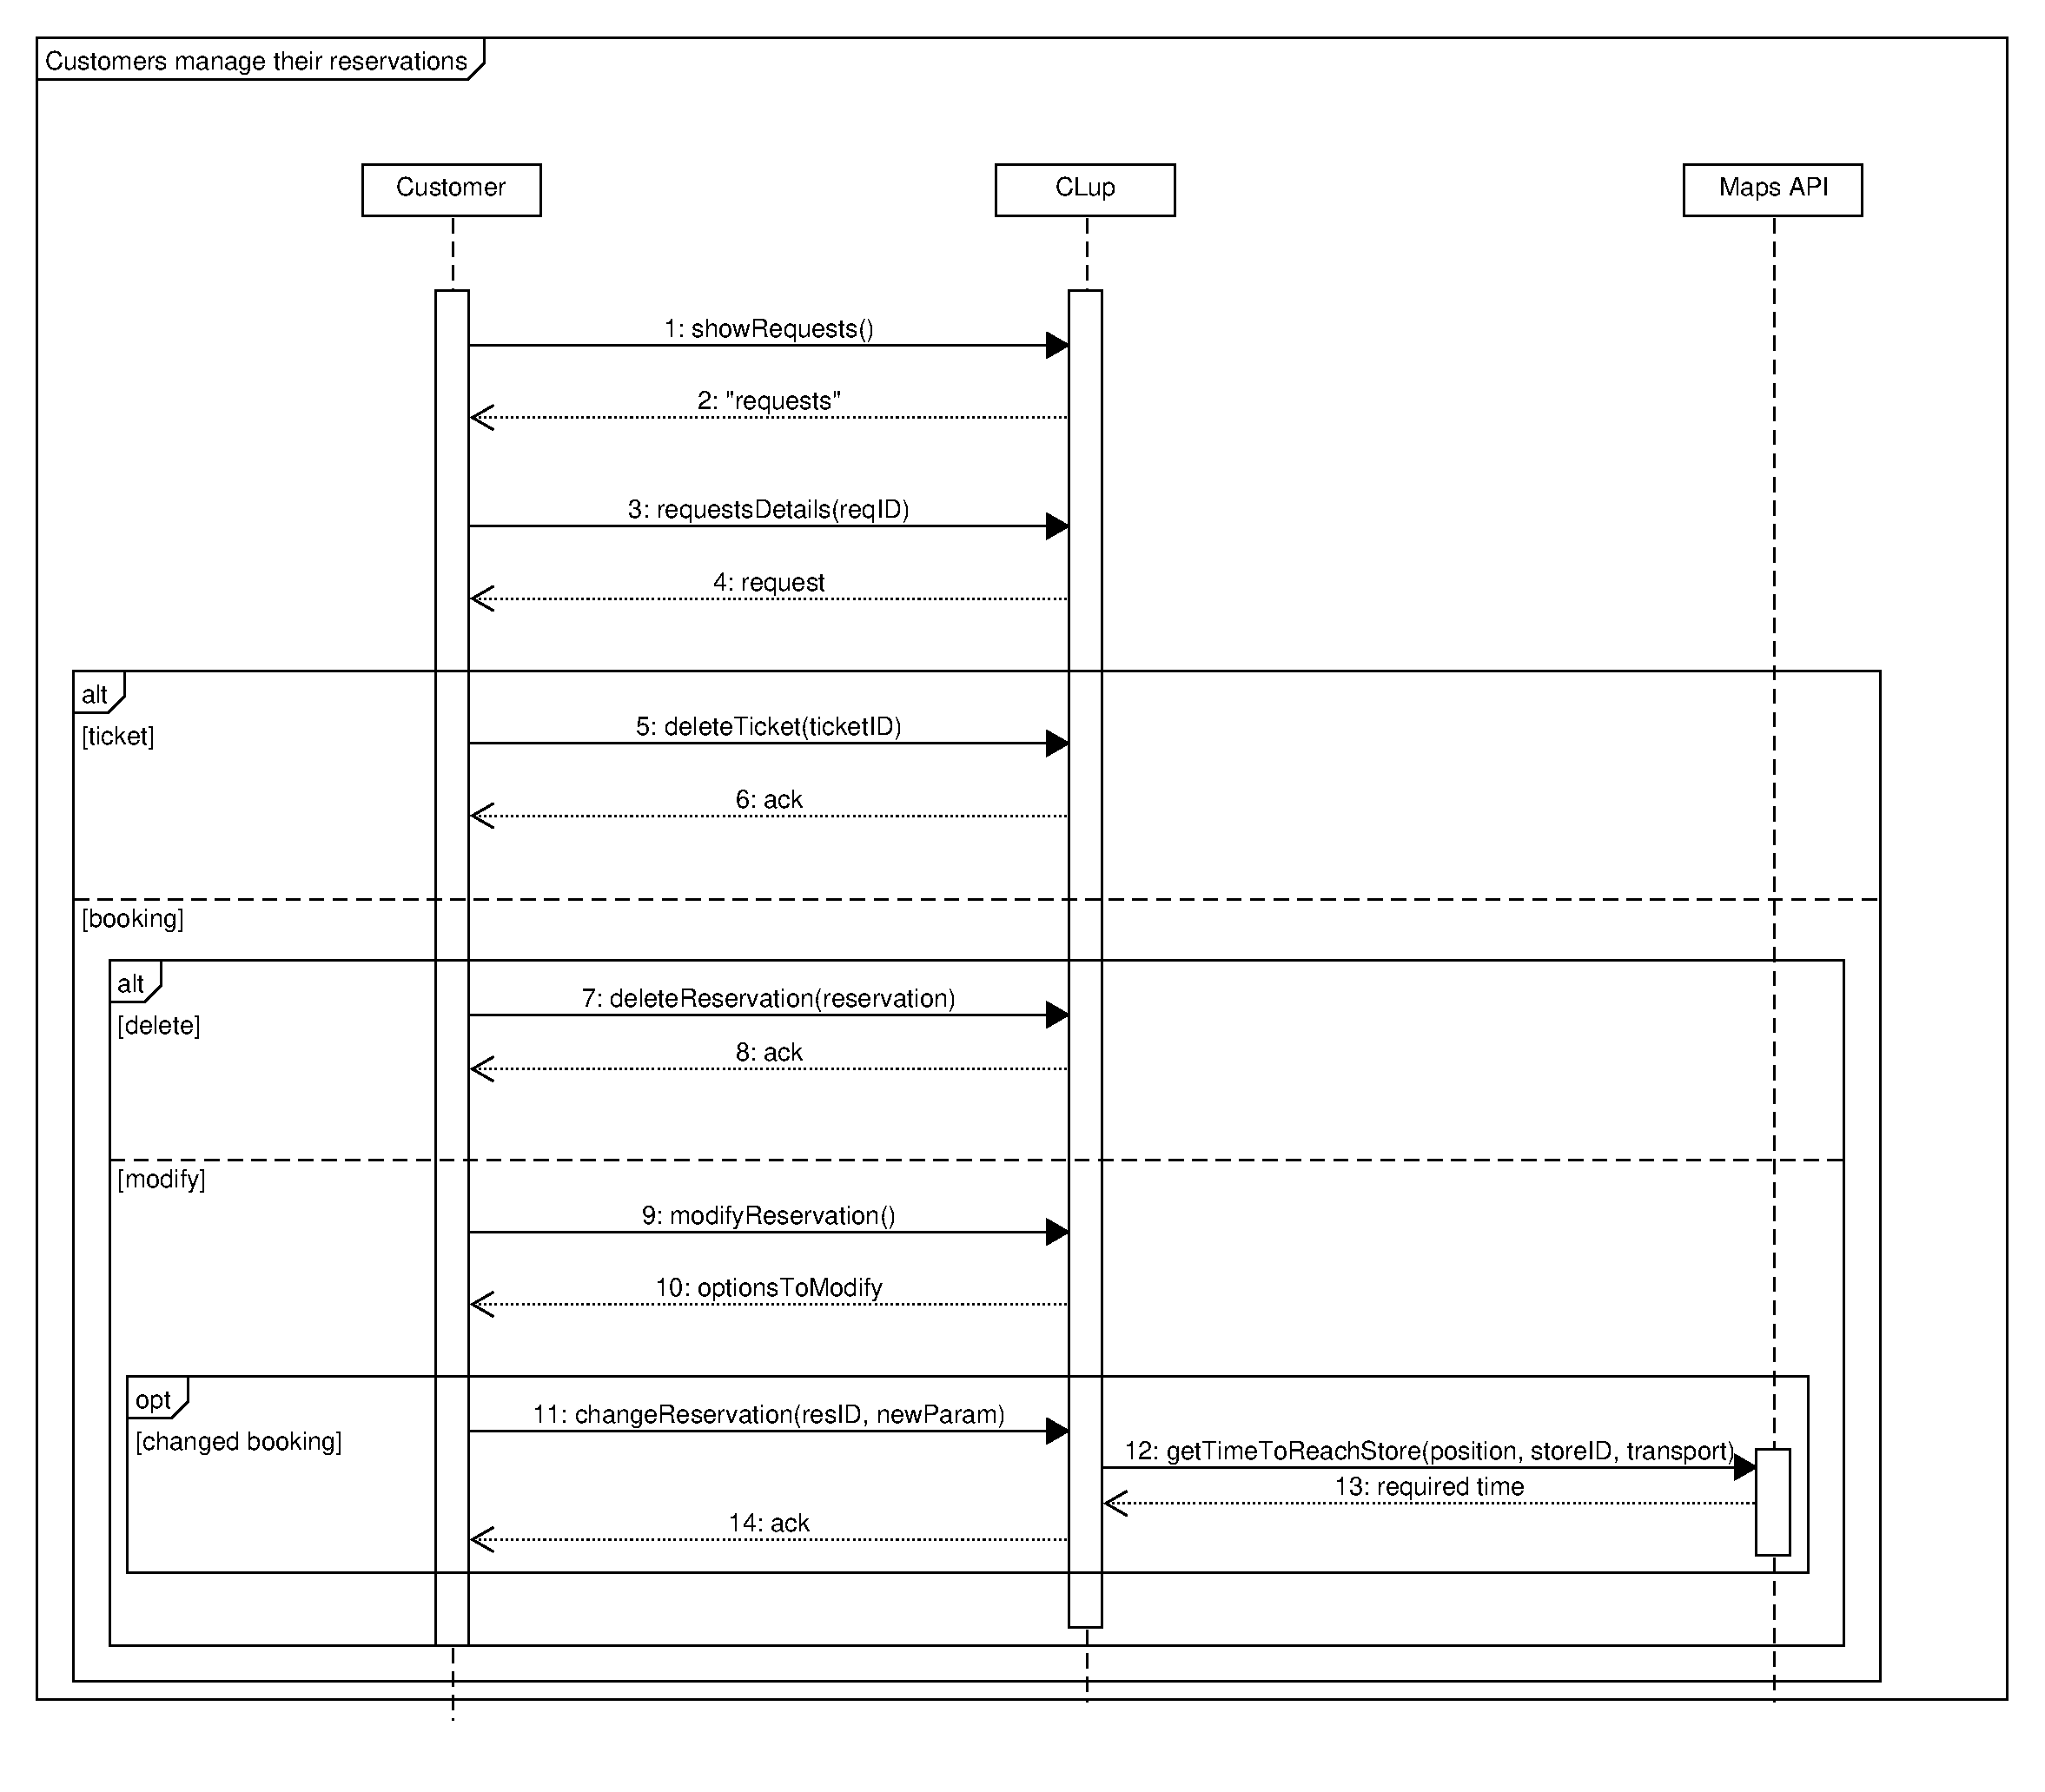
\includegraphics[scale=0.5]{SD/10_manageReservation(customer).pdf}\\
					\caption{Sequence Diagram of managing reservations customer side}
				\end{adjustwidth}
			\end{figure}
		\newpage
		
			\paragraph{Customer get a ticket with the totem}
			
				\begin{center}
					
					\rowcolors{2}{}{gray!20}
					\rowcolors{1}{gray!20}{white}
					
					\begin{adjustwidth}{-2.8cm}{}
					\begin{tabular}[h!]{|m{7.5em}|m{36em}|}
							\hline
							\xrowht{5pt}
							Name & Customer get a ticket with the totem\\
							\xrowht{5pt}
							Actors & Customer\\
							\xrowht{5pt}
							Entry Condition & The customer is at the store and is using the totem \\
							\xrowht{5pt}
							Event Flow & \begin{enumerate}
								
								\itemsep-0.25em
								\item Customer clicks the button “Get Ticket”
								
								\item Customers can see the list of all possible objects’ categories and can select some of them (optional)
								
								\item The customer enters the estimation of shopping time, or let the system to infer it
								
								\item Client confirms the options selected and the system generates and prints the associated number, the \emph{QR Code} and the \emph{ETA}
								
							\end{enumerate}\\
							\xrowht{5pt}
							Exit Conditions & The client gets a ticket \\
							\xrowht{5pt}
							Exception & \begin{enumerate}
								
								\item Client has not completed the operation in the prefixed time
								
							\end{enumerate}
						
							If the above situation occur, the application will throw an error message and will return to “Home” page \\
							\hline
							
						\end{tabular}
					

				
					\end{adjustwidth}
				
														\begin{itemize}
					\bigskip
					\bigskip
					\bigskip
					\bigskip
					{\bfseries Required functional requirements: }
					
					
					\item {\bfseries R9: } The system allows the customers to select some or all the de-
					partments in which the customers are interested in doing shopping
					\item {\bfseries R11: } The system must consider the extimate shopping time insert
					by customers
					\item {\bfseries R13: } The system have to make a reasonable estimate of when a user with a spot on the queue is able to enter the store
					\item {\bfseries R26: } The system is able to print a paper ticket
					\item {\bfseries R27: } The system can reasonably estimate the time needed from a specific user to complete his shopping
					\item {\bfseries R28: } The system must save clients' tickets
					\item {\bfseries R29: } The system should estimate when it must stop generating other tickets to avoid turns after the closing time of the store
					
					
					
					
				\end{itemize}
								\begin{figure}[!htb]
						\begin{adjustwidth} {-2,7cm}{}
							\centering
							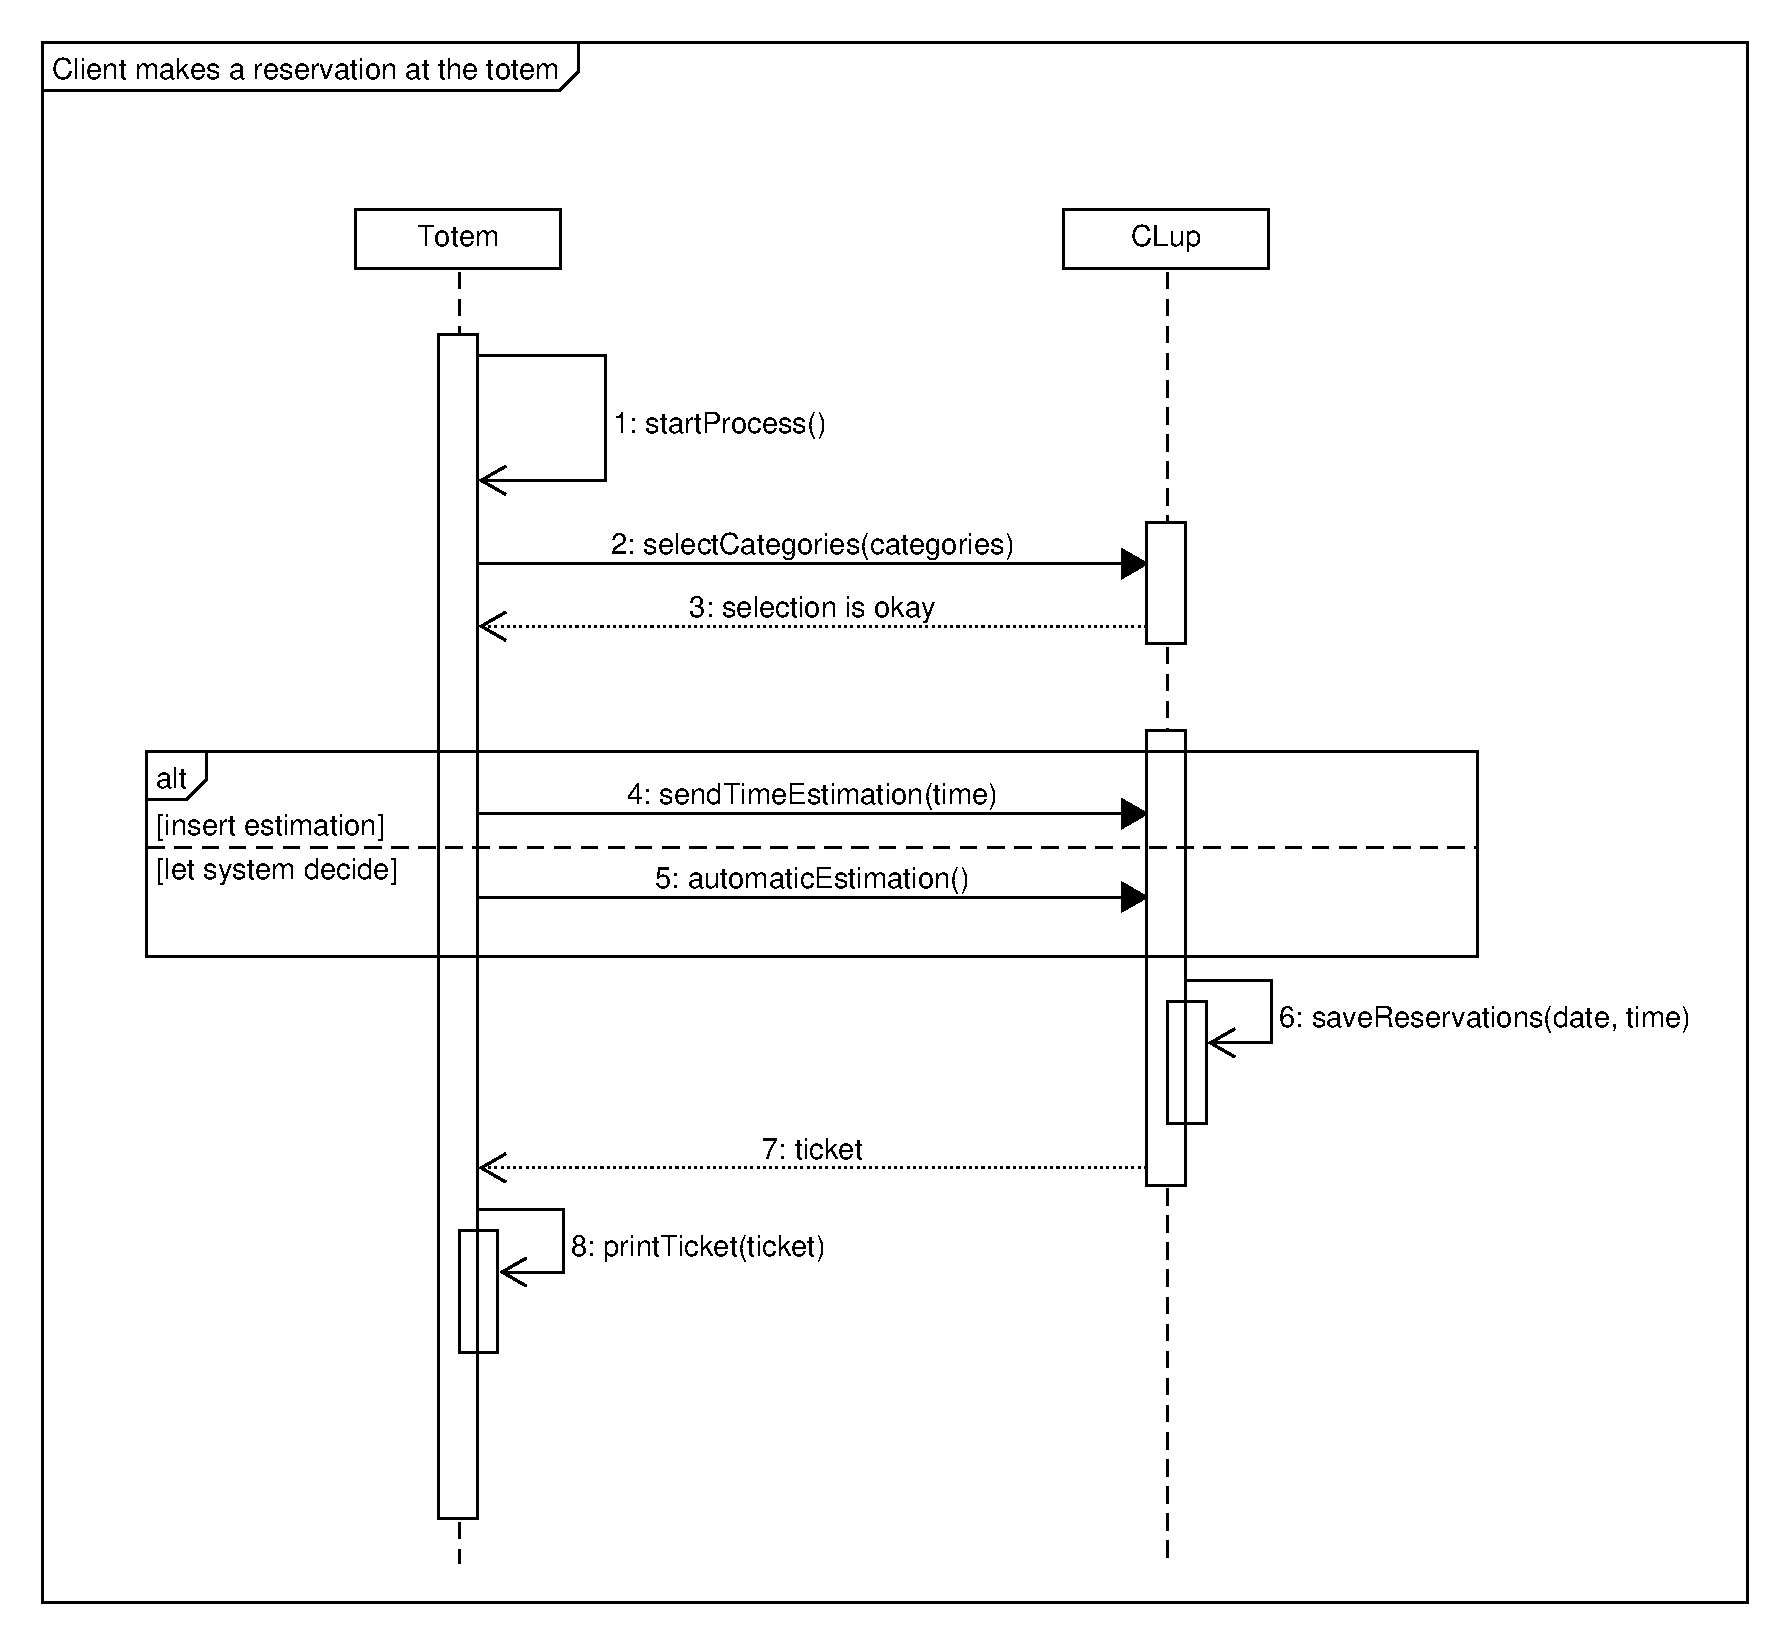
\includegraphics[scale=0.56]{SD/11_getTicketAtTotem.pdf}\\
							\caption{Sequence Diagram of getting a ticket at a physical dispenser}
						\end{adjustwidth}
					\end{figure}
				\end{center}
			\newpage
			\paragraph{Customer selects the prefered means of transport}
			
				\begin{center}
					
					\rowcolors{2}{}{gray!20}
					\rowcolors{1}{gray!20}{white}
					
					\begin{adjustwidth}{-1.5cm}{}
						\begin{tabular}[h!]{|m{7.5em}|m{27.5em}|}
							\hline
							\xrowht{5pt}
							Name & Customer selects the prefered means of transport \\
							\xrowht{5pt}
							Actors & Customer \\
							\xrowht{5pt}
							Entry Condition & Customer is already logged in the application service \\
							\xrowht{5pt}
							Event Flow & \begin{enumerate}
								
								\itemsep-0.25em
								\item Customer clicks the “Means of transport” button
								
								\item Customer can see a list of means of transport
								
								\item Customer select his preferred means of transport
								
								\item The system gets his \emph{GPS} positions and checks if the selected option is available.
								
								\item The app saves the option and updates the notifies alerting customers when they should depart for the store. 
								
								 
								
							\end{enumerate}\\
							\xrowht{5pt}
							Exit Conditions & The client selects the preferred mean of transport \\
							\xrowht{5pt}
							Exception & \begin{enumerate}
								
								\item The selected means of transport is not available
								
							\end{enumerate}
							
							If the above situation occur, the application will throw an error message and will ask the client to redo the selection \\
							\hline
							
						\end{tabular}
					\end{adjustwidth}
					
					\begin{figure}[!htb]
						\begin{adjustwidth} {-0,5cm}{}
							\centering
							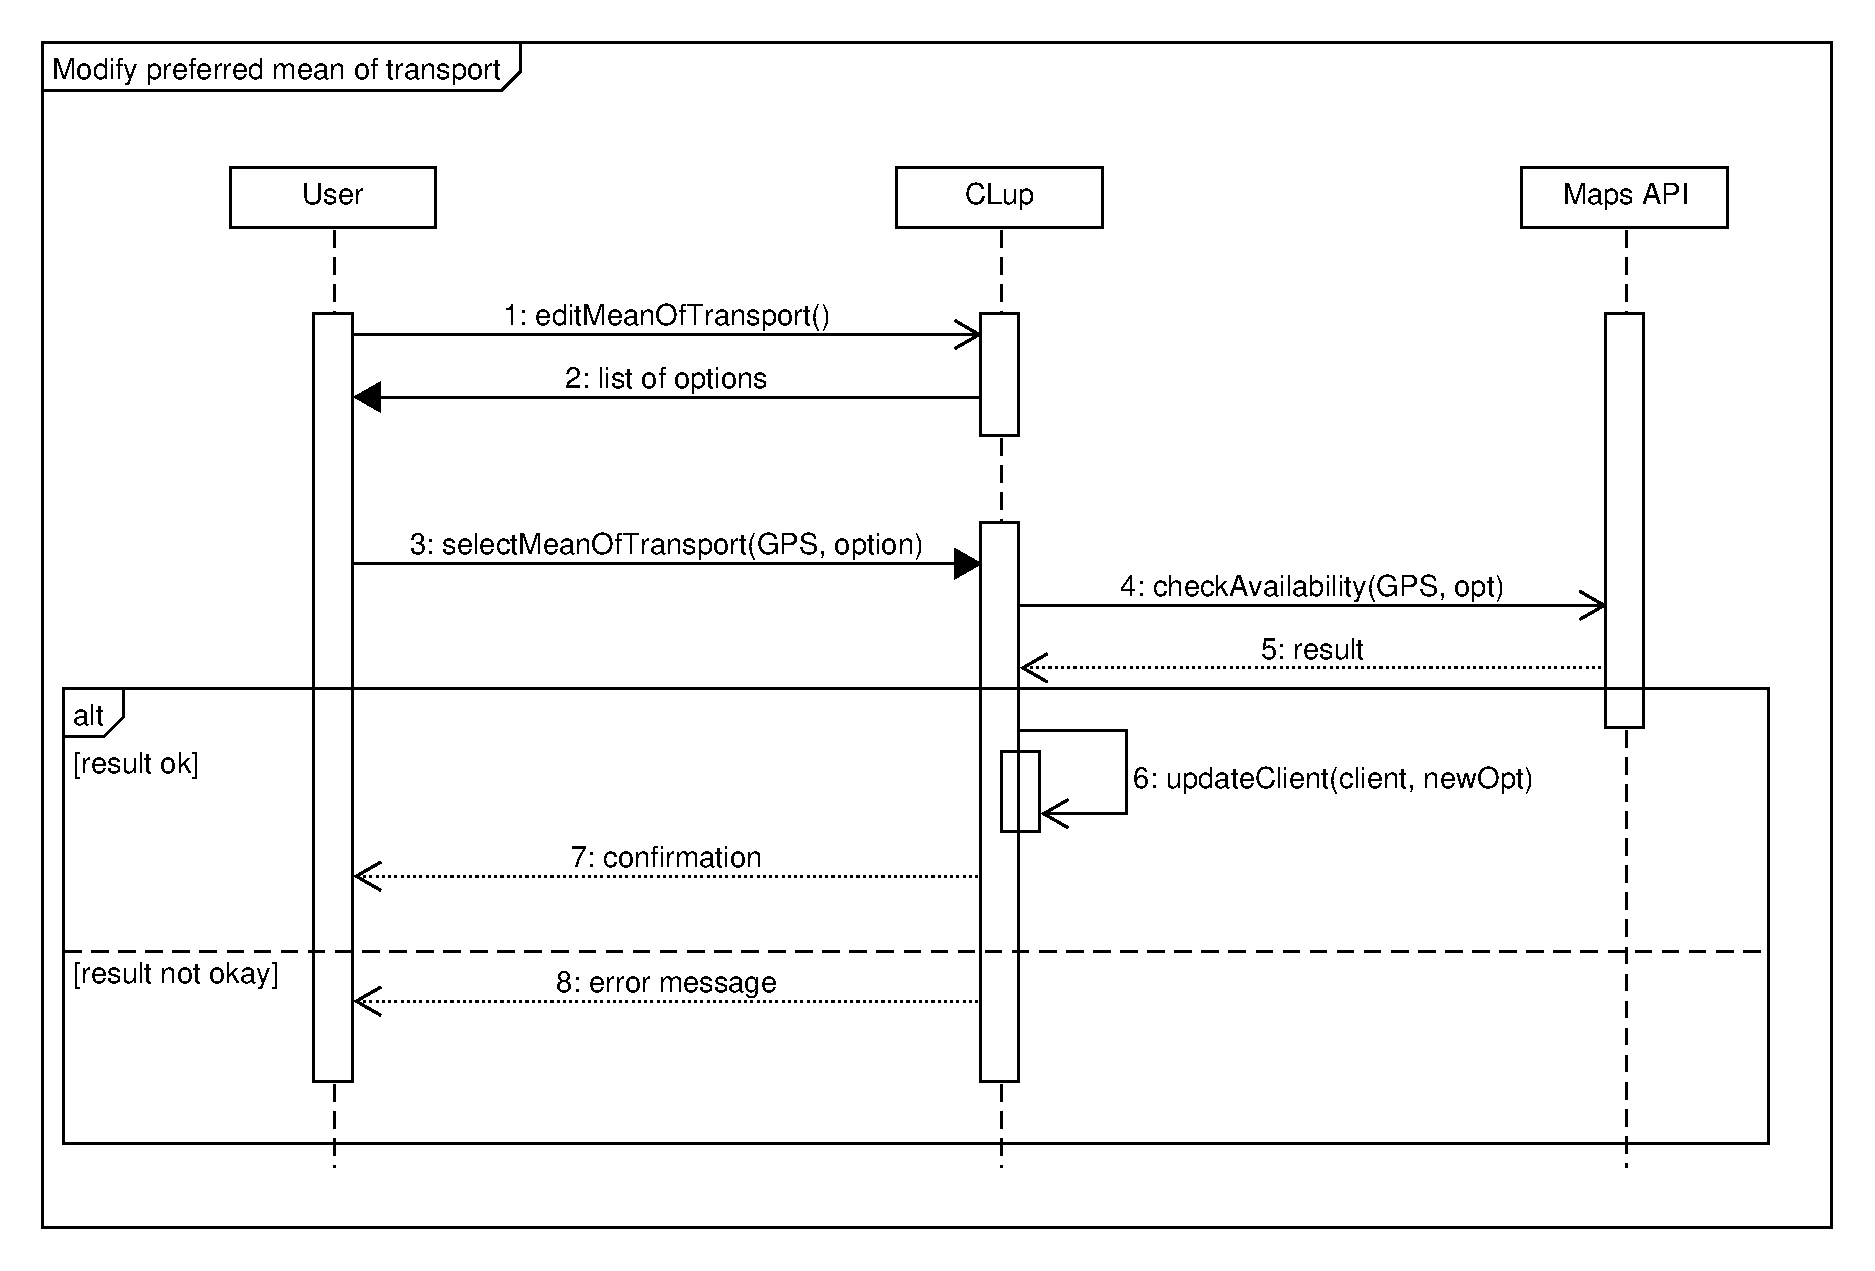
\includegraphics[scale=0.42]{SD/12_selectPreferredMeanOfTransport.pdf}\\
							\caption{Sequence Diagram of changing preferred mean of transport}
						\end{adjustwidth}

					\end{figure}
					
					
					\begin{itemize}
						\medskip
						\newpage
						{\bfseries Required functional requirements: }
						
						
						\item {\bfseries R8: } The system allows the customers to select their favorite means of transportation
						\item {\bfseries R15: } The system is able to ask for the position of the customers
											
						
					\end{itemize}
				\end{center}
		
		\subsection{Use Case Diagram}
		
		\begin{figure}[!htb]
			\begin{adjustwidth} {-3,6cm}{}
				\centering
				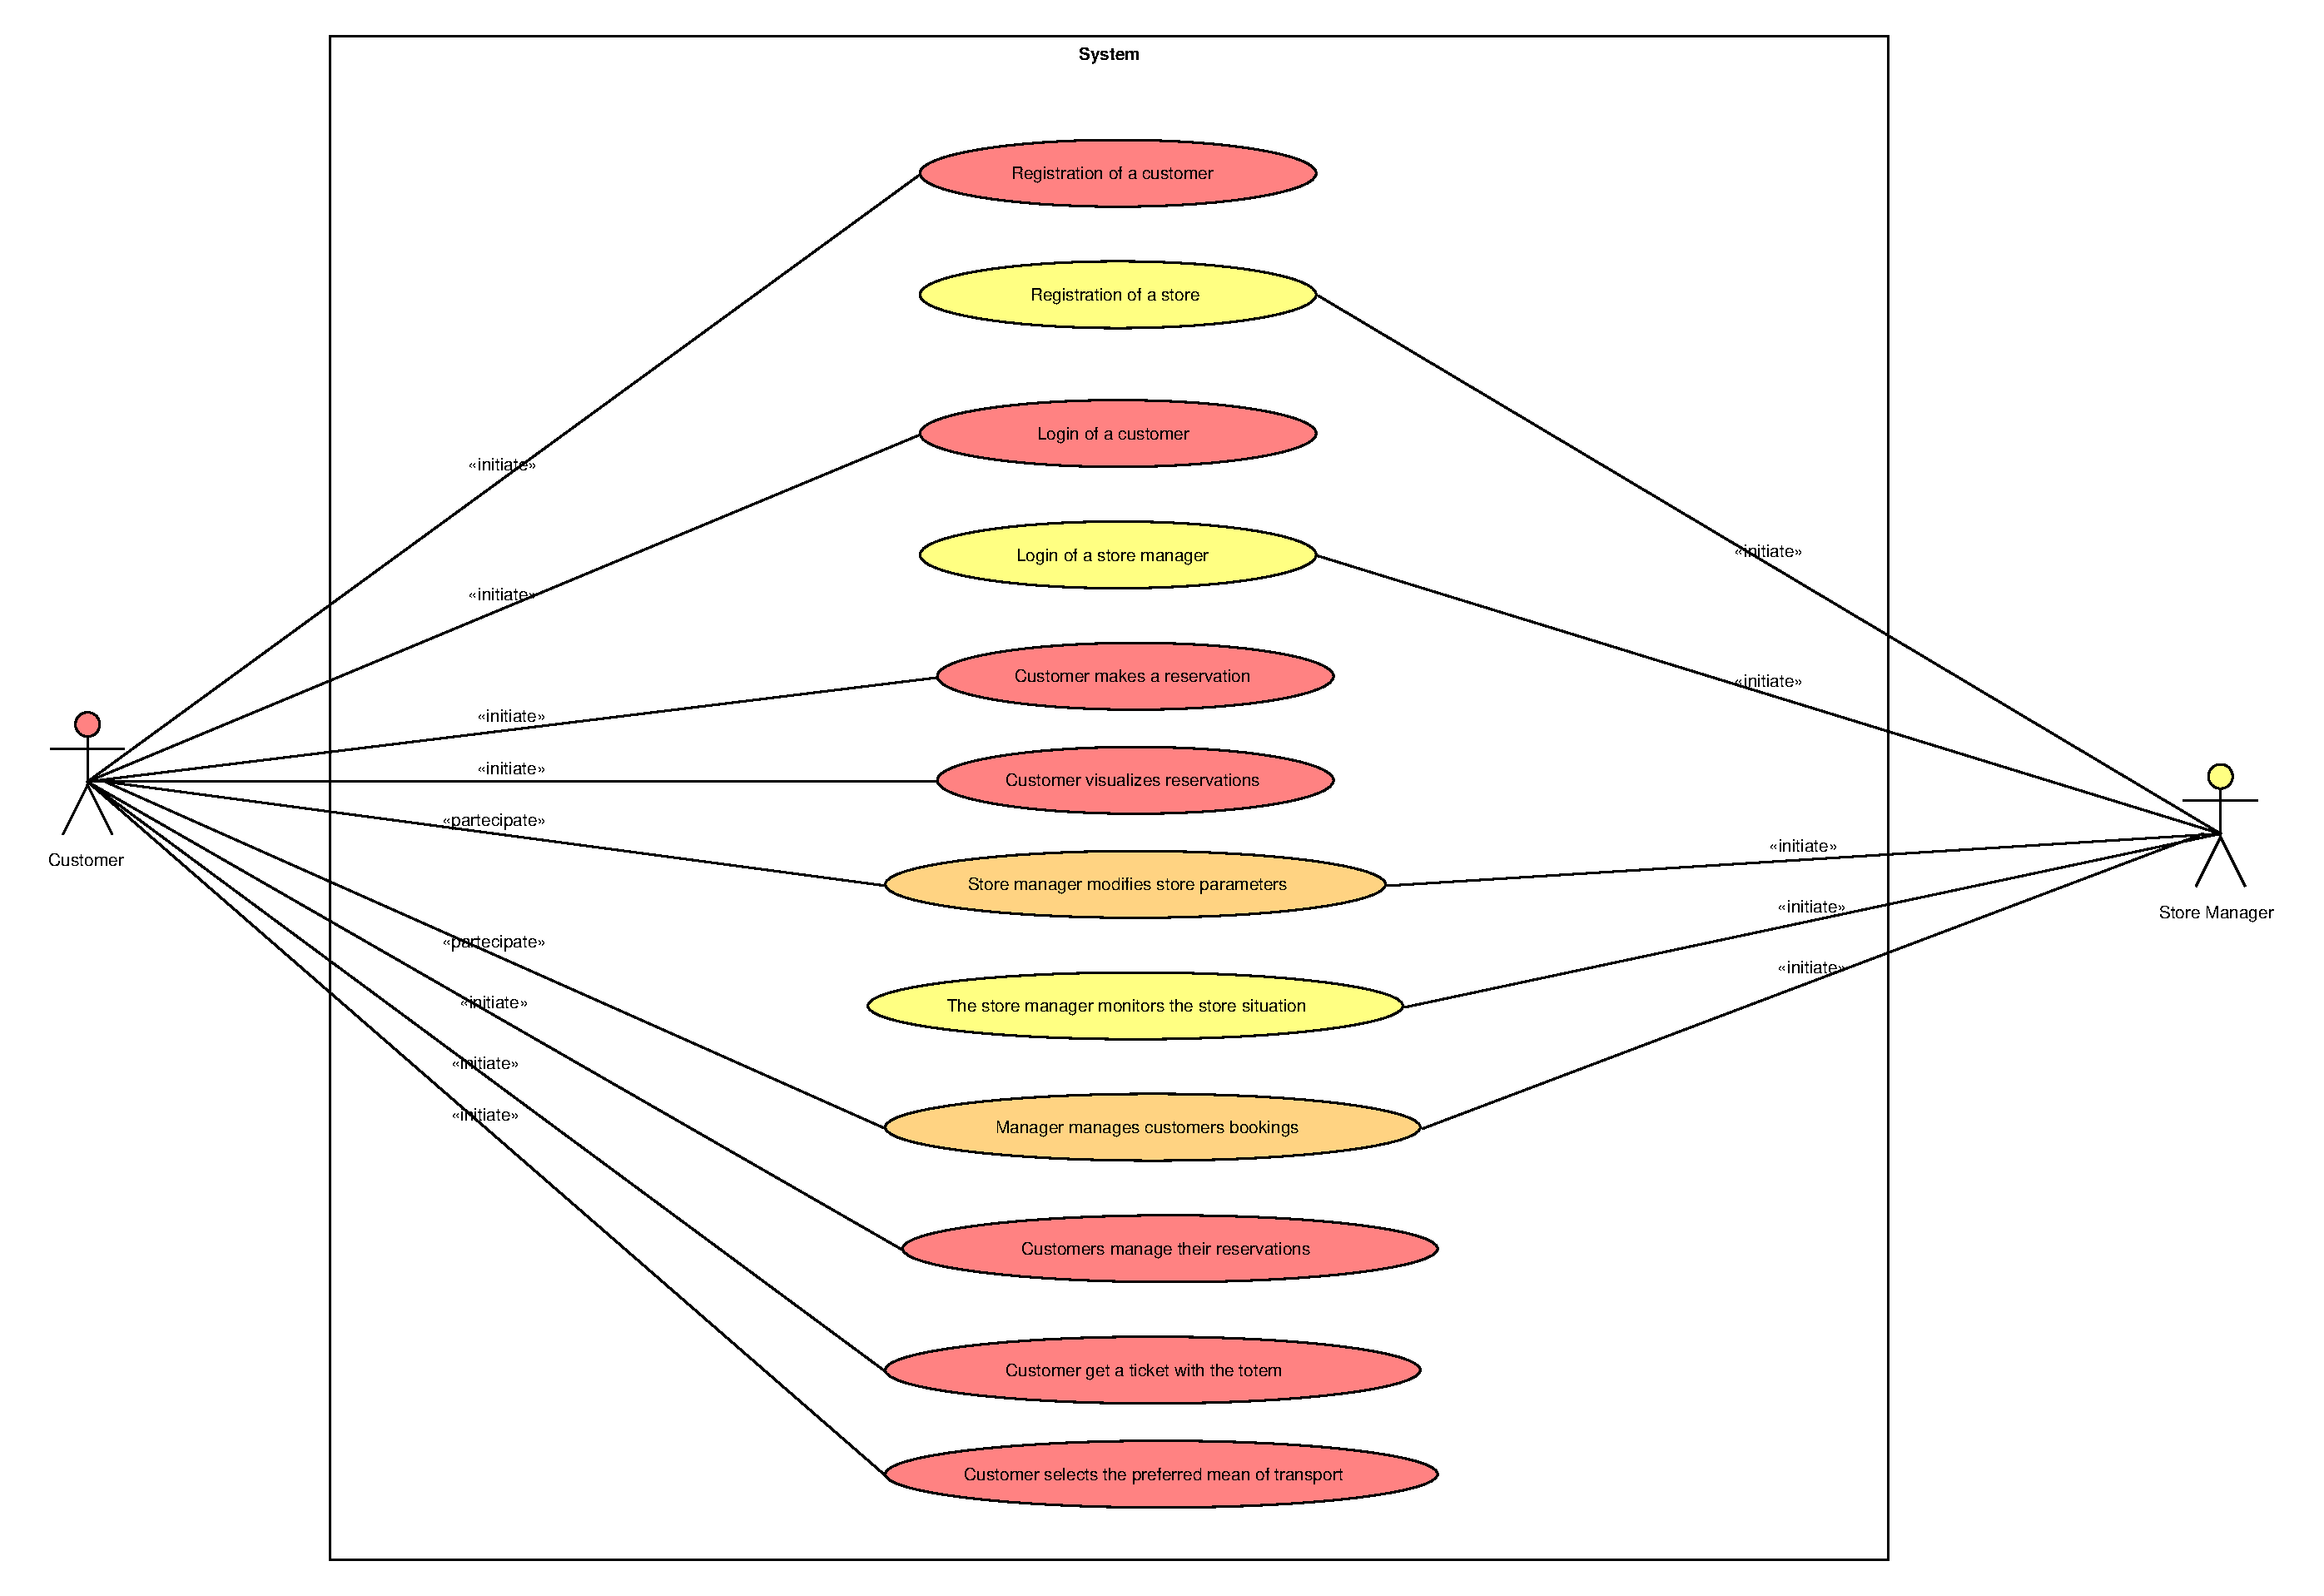
\includegraphics[scale=0.42]{UC/1_useCaseDiagram.pdf}\\
				\caption{Use Case Diagram}
			\end{adjustwidth}
			
		\end{figure}
		
		\subsubsection{Scenarios}
			
			{\bfseries Scenario 1: User without application} \\
			Marta is a university student unfavorable to consumerism and for this reason she does not have a smartphone. She go to her favorite store to do shopping and thanks to our system she can still book a place in the queue to enter in the store. To do this, she just go to the totem placed near the supermarket and fill in the reservation with the requested data, that is the departments she intends to visit and an estimate of the time spent inside the store. In this way, the system will queue her to enter as soon as possible, providing her with an estimated entry time. Knowing this, Marta can still do other activities before being called to enter the store, so as not to create crowds at the store exit. As with the app, Marta has to scan the ticket at the  entrance and exit. In this way the system can manage the queue and reservations. \\ \\
			{\bfseries Scenario 2: Fake QR code} \\
			Jonathan arrives at the store and notices that he has many people in line before him. Jonathan is not a very patient guy, so having kept another \emph{QR Code}, he tries to skip the line trying to scan it. The system recognizes that the \emph{QR Code} is not valid, therefore it does not allow Jonathan to enter the store, forcing him to respect the queue. \\ \\
			{\bfseries Scenario 3: User books from the application} \\
			Adalgiso must go shopping but does not want to wait a long time outside the store and wants to be sure that he can enter the moment he arrives. So, he opens CLup on his smartphone, sets up a preferred means of transport and begins a reservation. He Selects the store, the departments he wants to visit and the estimated time. Once the booking is complete, the app will send the notification to Adalgiso, inviting him to depart from his position to go to the store in time. When he will arrive, his number will be called shortly.\\ \\
			{\bfseries Scenario 4: Store manager have to smartly manage accesses} \\
			Apu is a store manager whose work is made more difficult by the current pandemic, since he has a small shop and no ways to manage crowds. Thanks to our application, now Apu is able to avoid assembles in front his store, he doesn't worry anymore about the number of people inside the store, and thanks to the statistics, he is able to regulate the number of allowed people and booked ones for each department of his small store.
		\newpage
	\subsection{Performance Requirements}
	CLup app is aimed to reduce gatherings due to the Covid-19 pandemic. So, some components needs a certain responsiveness. Here there are described some parts of the system that are critical to the scope of entire system
	\begin{itemize}
		\item {\bfseries Requests saving system:} when a client got a ticket, the system needs to process and save it in a very low time, less than 2 seconds,  since the requested tickets in a day are really important to allow or deny people to get another ticket for the same day/book a visit in a certain moment of the day.  
		\item {\bfseries QR Code processing:} each customer must scan his QR Code when he enters the store. This means that, to avoid delays in the queue, the component processing QR Codes must be really fast, and process them in no more than 5 seconds after the code is retrieved from the optical scanner.
		\item {\bfseries Ticket calling system:} as for QR Codes processing, after a customer exits the store, the system must be able to process the next ticket to be called, if any, in a strict time, to avoid that people waits outside the store for long times. This process must not last more than 10 seconds.
		\item {\bfseries User notifier: } the system must responsively notify users that they must depart for the store in time. 
		\item{\bfseries Application data updates: } when the customer need to use the application for any purpose, the app must be responsive, and each object required over the network must be available in no more than 5 seconds from its request; if the retrieve from the net fails, the app will show the local stored data to avoid delays in the whole system (eg. the client must retrieve his QR Code to access the store) 
		\item{\bfseries Totem ticket printing: } the totem must process each request and print the ticket in no more than 5 seconds.
		
	\end{itemize} 

		The above reported performance constraints must be always verified; that implies the system must be highly scalable to respect this timing. There isn't any limit on the number of registered stores and users, so the system must respect these constraints with at least 200 connected users per each store inside the system.

	\newpage
	
	\subsection{Design Costraints}
	
		\subsubsection{Standards Compliance}
		
			System is compliant to some standards, such as:
	\begin{itemize}
		\item Generated QR Codes are compliant to ISO/IEC 18004:2015 standard
		\item Network messages are exchanged through the internet protocol TCP/IP
	\end{itemize}
The same doesn't applies to requests of travel times, since the uses non-standard API of some map service.
		\subsubsection{Hardware Limitations}
		To work properly, CLup needs some type of hardware, in base of the considered component.
		\begin{itemize}
			\item {\bfseries Customer Device:} Customer needs to have a device with a working network module, a GPS module and a high resolution display (minimum 720P).
			\item {\bfseries Totem:} the totem must have a working network module, a ticket printer and a module to make possible interfacing between customer and totem
			\item {\bfseries QR Code readers:} QR Code readers must have a working network module, and a optical scanner that takes no more than 5 seconds to read and interpret a QR code and its content
		\end{itemize}
	\subsection{Software System Attributes}
		\subsubsection{Reliability}
		The system must have a  very low probability of failure (less than 0,0001\%) to avoid inconveniences in crowd managing.
		\subsubsection{Availability}
		Due to the critic aspects the application handles, is required a 99,99\% of system reliability. It means that the application will be down only for 52.60 minutes per year, an estimate that is acceptable. Having a greater downtime per year, may lead to inconveniences in handling the queue outside a store, bringing to a possible assembly of people.
		\subsubsection{Security}
		Each communication between client and server is made over a secure transport protocol (eg. TLS). For each request the system will authenticate the user so that everyone access only to data he is authorized. An encryption and decryption system must be implemented so that QRs' Content is encrypted to avoid someone can forge a malicious ticket. Moreover, each user password is stored using its hash value. 
		\subsubsection{Maintainability}
		Since rules can change in every moment, the software must be developed in an extendible way, so that it'e easy to add new functions required by new restrictions. Moreover, the software can be used even if after the pandemic. So, it might be required to implement new feature to make the system more appealing.
		\subsubsection{Portability}
		The application must be portable on the majority mobile OSes. For this reasons, the app will use a notification service accessible through the OS APIs. Furthermore, the software is thought so that is possible to implement different map service in different versions.
		\subsection{Additional Specifications}
	The system guarantees unicity of each customer's email and of each store manager's ID.
	
	\newpage
	
\section{Formal Analysis Using Alloy}
	The following section considers the fundamental properties and constraints identified for the specification of the problem and formally define them with a formal model in which it is shown how they will be satisfied. The alloy modelling language is used to model the problem, and some possible comments are also provided in order to clarify the most critical aspects. 
	\subsection{Alloy Model}
	
	sig Username\{
	
		usr: one String
		
	\}
	
	
	sig Password\{
		
		psw: one String
		
	\}


	sig Email\{
	
		email: one String
		
	\}
	
	sig Name\{
	
		name: one String
		
	\}
	
	sig Surname\{
	
		surname: one String
		
	\}

	sig Certification\{\}
	
	sig CustomerReg\{
	
		username: one Username,
		
		password: one Password,
		
		email: one Email,
		
		name: one Name,
		
		surname: one Surname
		
	\}

	sig Customer\{
	
		registration: one CustomerReg
		
	\}

	sig StoreReg\{
	
		name: one Name,
		
		password: one Password,
		
		certification: one Certification,
		
		capacity: one Int		
		
	\}
	
	sig Store\{
	
		registration: one StoreReg
		
	\}
	
	
	
	
\section{Effort Spent}

\section{References}	
	
	
	
\end{document}